\chapter{Energy Estimators}
\label{chap:MoreStuff}

\chapterquote{There, sir! that is the perfection of vessels!}
{Jules Verne, 1828--1905}

%========================================================================================
%========================================================================================

\section{Calibration}

%========================================================================================

\subsection{Calibration in the particle flow paradigm}
% Results use detector model 85 and calibration variant 71

In any experiment, calibration is essential for ensuring reliability in measured quantities and the linear collider will be no exception to this.  In the particle flow paradigm measured energy deposits fall into two distinct classes (i) calorimetric energy deposits and (ii) charged particle tracks.  Calorimetric energy deposits are the essential building blocks for the application of the particle flow.  The separation of energy deposits from charged and neutral particles in the calorimeters is crucial for achieving good energy resolutions and this is only possible if the energy estimators for those energy deposits are accurate.  

%The other crucial energy deposit used in particle flow calorimetry are track energy deposits.  These are also crucial to physics performance, however, in the particle flow paradigm these energy deposits are topologically related to the energy of the reconstructed particle.  A spatial helix fit is applied to the track energy deposits which when combined with knowledge of the magnetic filed yields the momentum of the particle producing the track.  Therefore, there is no direct relationship between the energy deposited by the monte-carlo particle in the active medium and the energy of the reconstructed energy.  Therefore, precise calibration of the energy deposited by a charged particle track is less crucial than for calorimeter energy deposits.  For this reason the focus of this chapter is on the calibration of calorimeter energy deposits. 

Calibration of the linear collider detector simulation extends beyond the calorimeter hits and into the particle flow algorithm itself.  The fine calorimeter granularity required for particle flow calorimetry yields excellent separation of hadronic and electromagnetic showers.  The pattern recognition software used in the reconstruction, PandoraPFA, provides detailed particle identification that allows for distinct treatments of electromagnetic and hadronic particle shower energy estimators.  This distinction can be used to produce a response from the calorimeter that is compensating, i.e. a calorimeter that has an identical response to electromagnetic and hadronic showers initiated by particles of the same incident energy, despite the intrinsic response being non-compensating.  This would significantly improve the energy resolution of the detector and extend the physics potential of the linear collider experiment.  Therefore, incorporated within the calibration procedure is the setting of several, energy independent, rescaling factors.  These factors are applied to the energy measurements from electromagnetic and hadronic particle showers with the aim of achieving a compensating calorimeter response.  

It is possible to make further improvements to the energy resolution by applying energy corrections during the reconstruction.  With that aim in mind a study into two energy correction options will be presented.  These studies show the effect of the corrections on the energy resolution of the detector as well as the pattern recognition aspect of the reconstruction.  The first energy correction to be studies is a naive energy truncation for calorimeter cells in the HCal, while the second, software compensation, is a more sophisticated approach involving the use of the energy density of the calorimeter hits to determine an energy correction.  

The chapter concludes with a discussion of the impact of timing cuts applied to calorimeter hits in the software trigger for the linear collider.   

Details regarding how all the detector performance metrics used in this chapter are calculated can be found in section \ref{sec:optstudiesmetric}.

%========================================================================================

\subsection{Calibration and detector optimisation}
Optimising the detector at a future linear collider will be crucial to exploit the full physics potential available to it.  An extensive optimisation of the calorimeters was performed and the results can be found in chapter \ref{sec:optimisationstudies}.  For each detector model considered in this study the calibration procedure outlined in this section was applied to ensure optimal performance was achieved.  This made unbiased comparison between detector models performance possible and ensured reliability in the conclusions drawn from this study.

%========================================================================================

\subsection{Calibration Goals}
The calibration procedure aims to determine variables related to four aspects of the reconstruction, which are:

\begin{enumerate}
\item \textbf{Digitisation of calorimeter hits}.  Digitisation in this sense is the estimation of the energy deposited within a calorimeter cell, both the active and absorber layers, based on the signal measured in the sensitive region of the cell, the active layer.  
\item \textbf{Minimum ionising particle (MIP) scale setting in the digitisation processor and PandoraPFA}.  The MIP scale has to be set in the digitiser as it simulates the response of the readout technology, which includes a maximum readout value set in units of MIPs.  The digitiser also applies a minimum threshold on the active layer cell energy, in units of MIPs, for calorimeter hit to be created.  PandoraPFA uses the MIP scale to place further threshold cuts on the cell energy that must be exceeded for a calorimeter hit to be used in the reconstruction.  Both of these thresholds are designed to veto noise that would be present in a real detector.  While noise is not applied in these simulations, the cuts are applied to better reflect the performance of a real detector. 
\item \textbf{Electromagnetic and hadronic scale setting in PandoraPFA}.  As discussed in chapter CALORIMETER CHAPTER, the response of a calorimeter to electromagnetic and hadronic showers is different due to the fundamentally different mechanisms governing their propagation.  A key difference between the two is the presence of an invisible energy component within hadronic showers.  This leads to calorimeters to produce a lower response to hadronic showers than to electromagnetic showers initiated by particles of the same incident energy.  To account for this and any energy losses incurred due to the application of noise vetoing cuts in PandoraPFA the PFO energies are rescaled depending on whether the PFO has showered electromagnetically or hadronically.  Determination of these scaling factors is the setting of the electromagnetic and hadronic energy scales.  
\item \textbf{Retraining photon likelihood data}.  The PandoraPFA algorithm uses likelihood data to determine whether a reconstructed object is a photon.  This likelihood data has to be retrained every time the ECal is altered.
\end{enumerate}

The majority of these aspects must be addressed every time the detector model changes.  The ordering of each of these calibration steps is also crucial as it is possible to get interference between the different stages if applied in an arbitrary order.

%========================================================================================

\subsection{Digitisation}
\label{sec:digi}
Calibration of the digitisation of the calorimeter hits involves accurately estimating the energy deposited in a calorimeter cell, in both the active and absorber layers, based on the energy deposited in the sensitive element of the calorimeter, the active layer.  The relationship between the energy deposited in the active layers and the absorber layers of a calorimeter is linear as the energy deposited in both layers is proportional to the number of charged particle tracks passing through them.  This works under the assumption that the density of charged particle tracks across a calorimeter cell within a particle shower is uniform.  The ratio of the calorimeter cell energy to the energy deposited in the active layers is hereby called the digitisation constant.

The digitisation constant for a calorimeter depends upon factors including the material properties of the calorimeters, the magnetic field strength and energy losses occurring within the gaps between the active and absorber layers.  To account for the extra material in the detector due to the effect of instrumented read out technology additional material surrounding the active and absorber layers is added in the simulation of the calorimeters.  In comparison to the absorber layer, this extra material adds little to the detector, however the small energy losses incurred here will be accounted for by the digitisation calibration.  

%========================================================================================

\subsubsection{ECal Digitisation}
\label{sec:ecaldigi}
The procedure for determining the digitisation constants in the ECal involves simulation of single $\gamma$ events at energy $E_{MC} = 10$ GeV.  $\gamma$ events are ideal for the calibration of the ECal as $\gamma$ energy measurements are made primarily within the ECal.  Furthermore, at this energy, $\gamma$s are largely fully contained within the ECal, as shown in figure \ref{fig:ecaldigiphotonsplit}.  This makes them ideal for isolating the ECal digitisation calibration from that of the HCal digitisation calibration.   

\begin{figure}
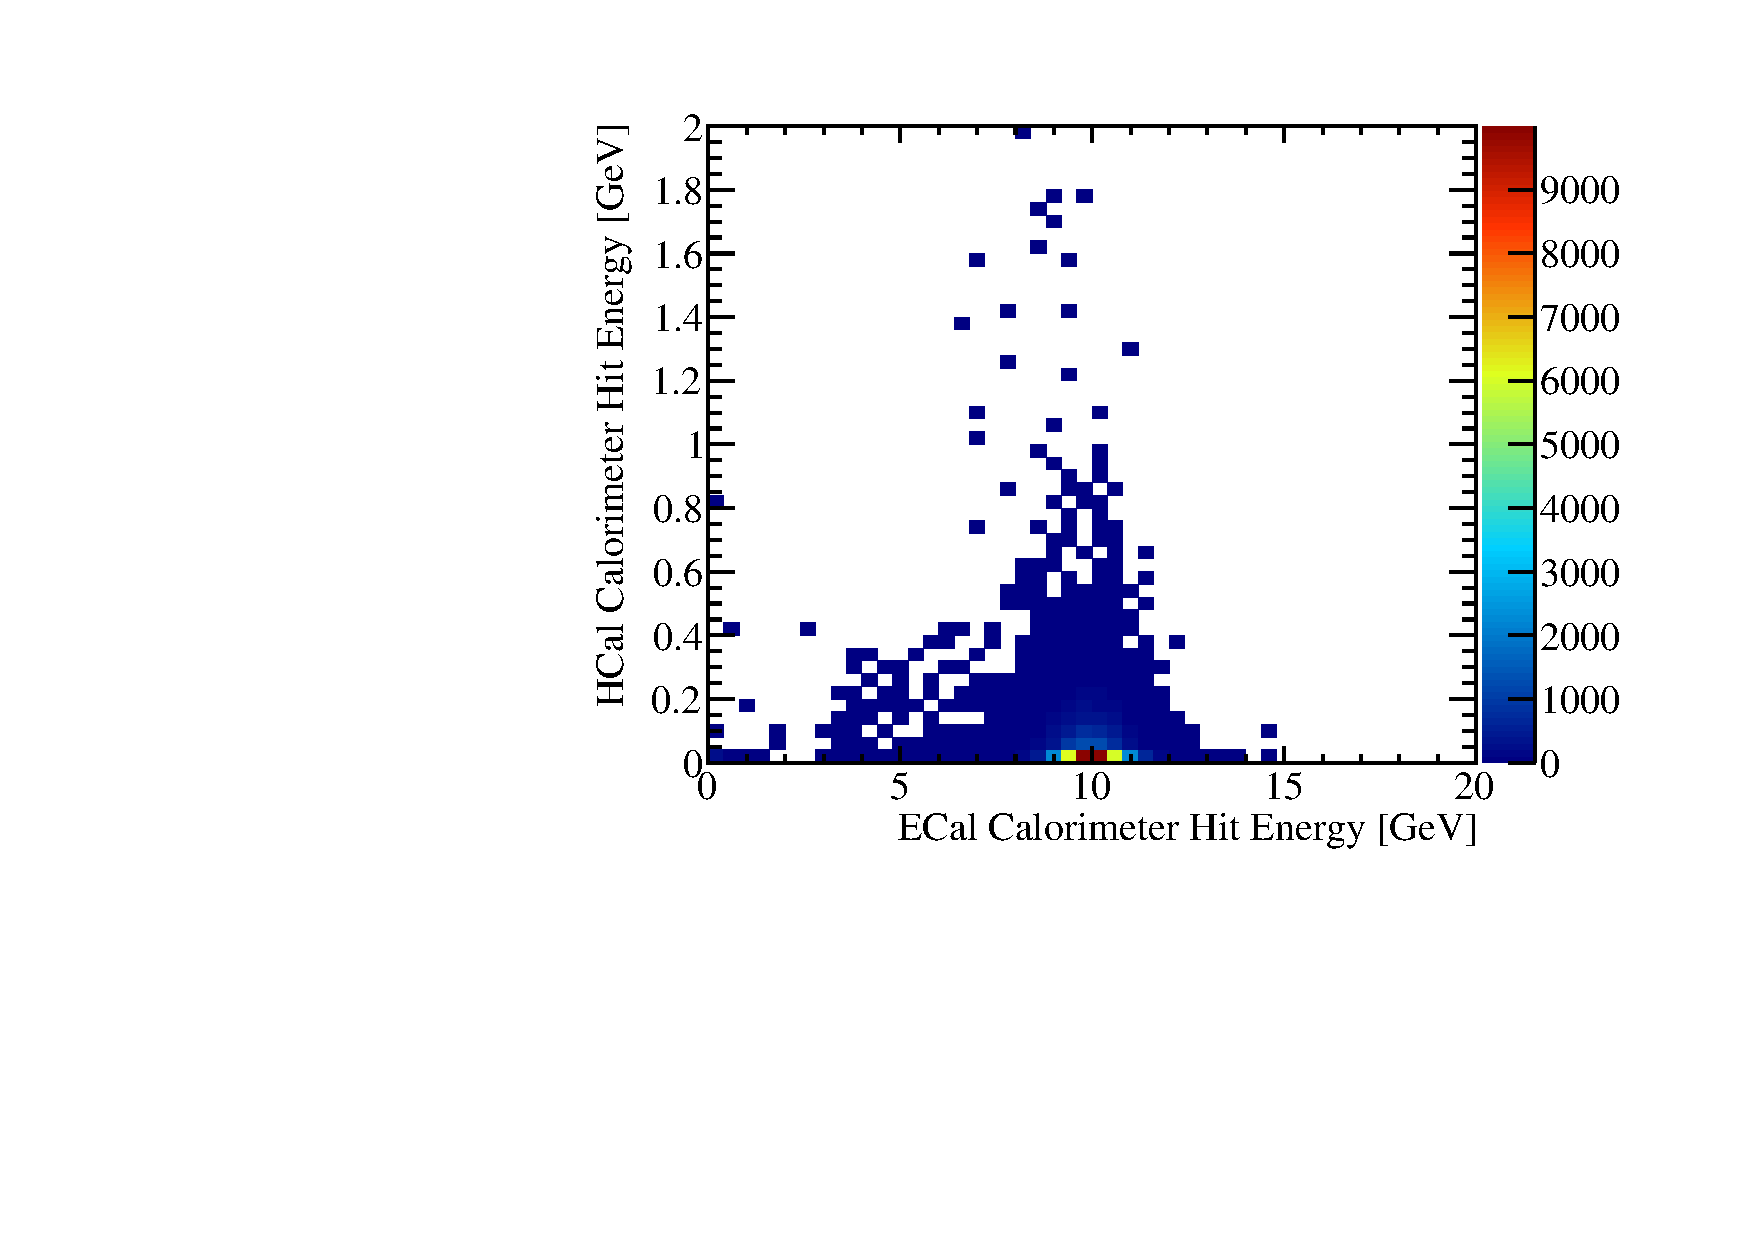
\includegraphics[width=0.5\textwidth]{EnergyEstimators/Plots/Calibration/Digitsation/ECal/ECalHCalPhotonSplit.pdf}
\caption[The sum of calorimeter hit energies in ECal and HCal for 10 GeV $\gamma$ events.]{The sum of calorimeter hit energies in ECal and HCal for 10 GeV $\gamma$ events.}
\label{fig:ecaldigiphotonsplit}
\end{figure}

Events are only used for calibrating the ECal digitisation if they are confined to the ECal.  To that extent cuts are applied ensuring that the sum of any reconstructed energy found outside the ECal is less than 1\% of $E_{MC}$ and that the $\text{cos}(\theta) < 0.95$ where $\theta$ is the polar angle of the $\gamma$.  $\gamma$ conversions are also vetoed in this event sample at MC level.  The impact of these cuts on the sum of ECal hit energies for the $E_{MC} = 10$ GeV $\gamma$ events is shown in figure \ref{fig:ecaldigiselection}.

\begin{figure}
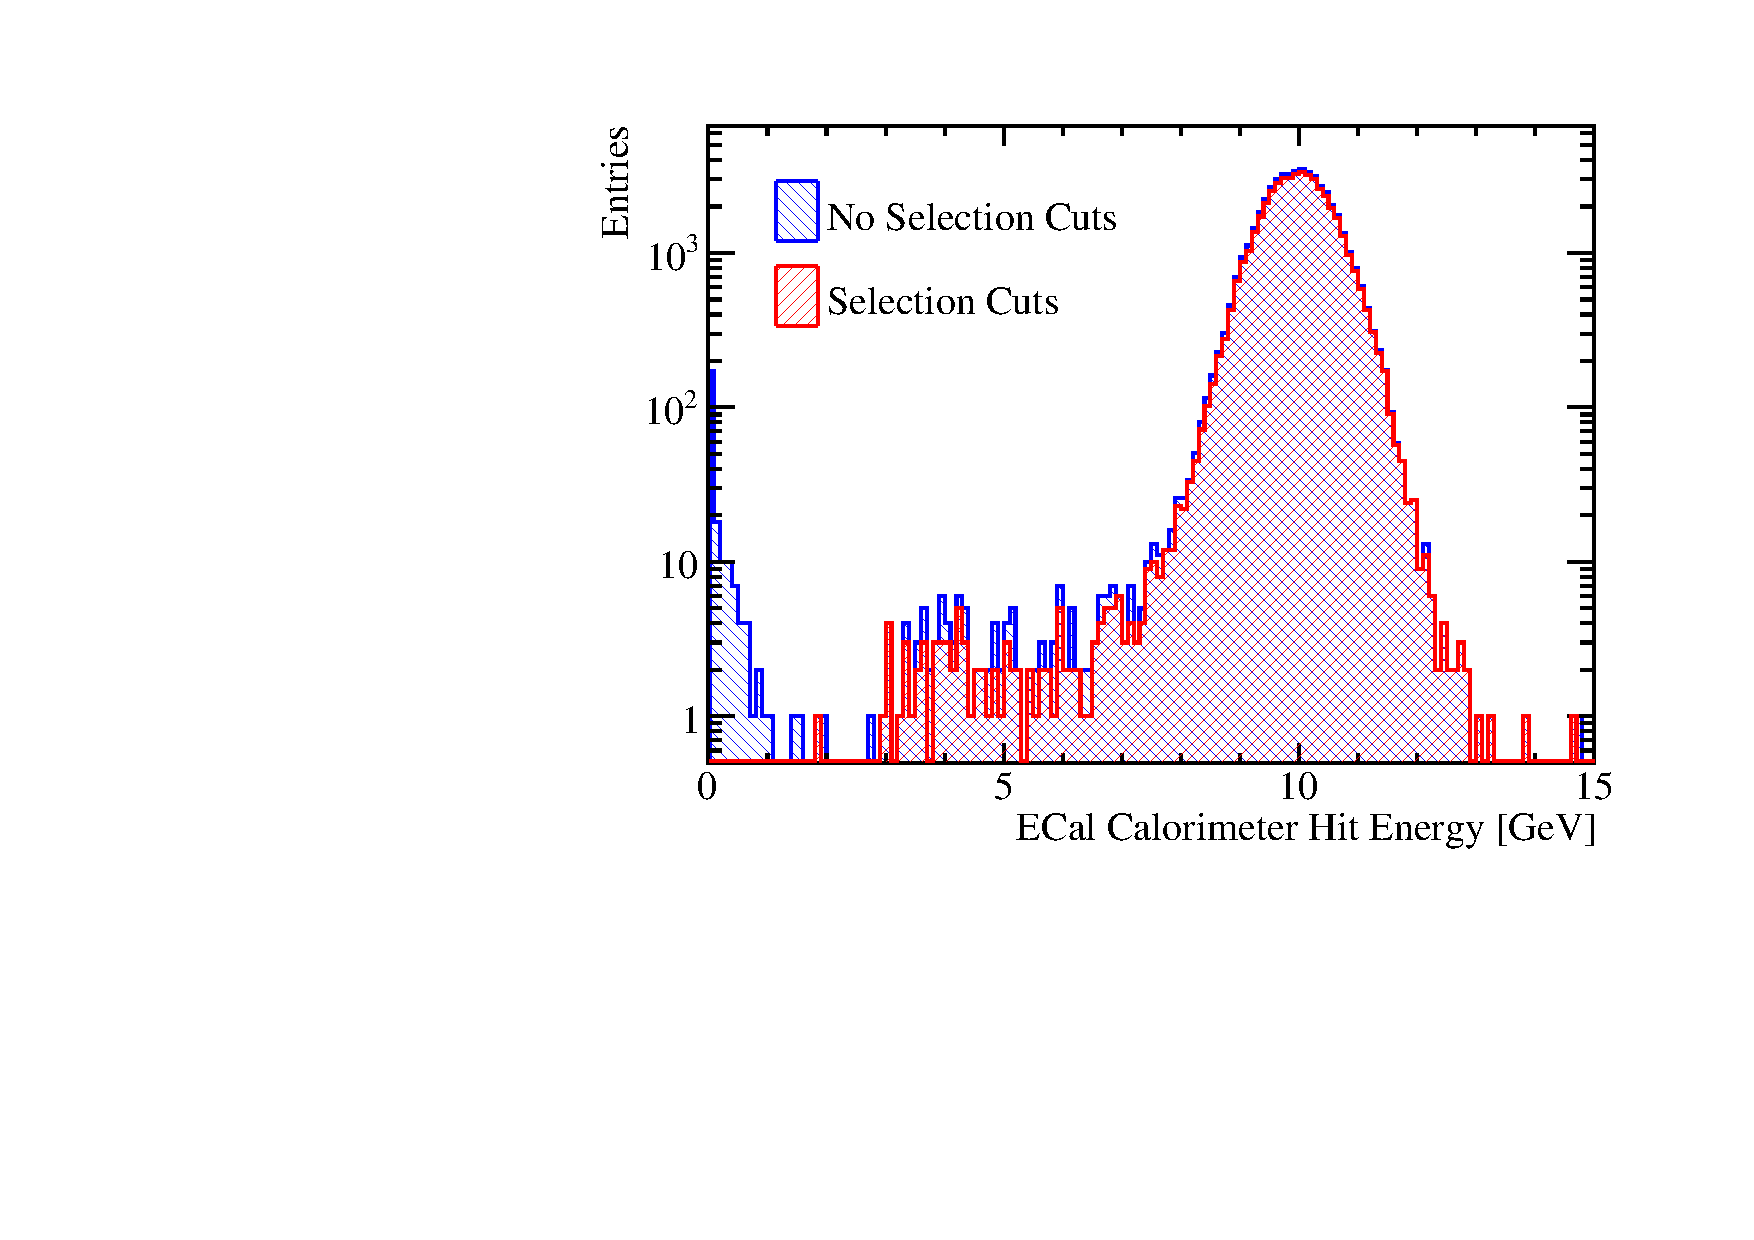
\includegraphics[width=0.5\textwidth]{EnergyEstimators/Plots/Calibration/Digitsation/ECal/DigitisationECalSelection.pdf}
\caption[The sum of the ECal calorimeter hit energies for 10 GeV $\gamma$ events with and without the selection cuts.]{The sum of the ECal calorimeter hit energies for 10 GeV $\gamma$ events with and without the selection cuts.}
\label{fig:ecaldigiselection}
\end{figure}

\begin{figure}
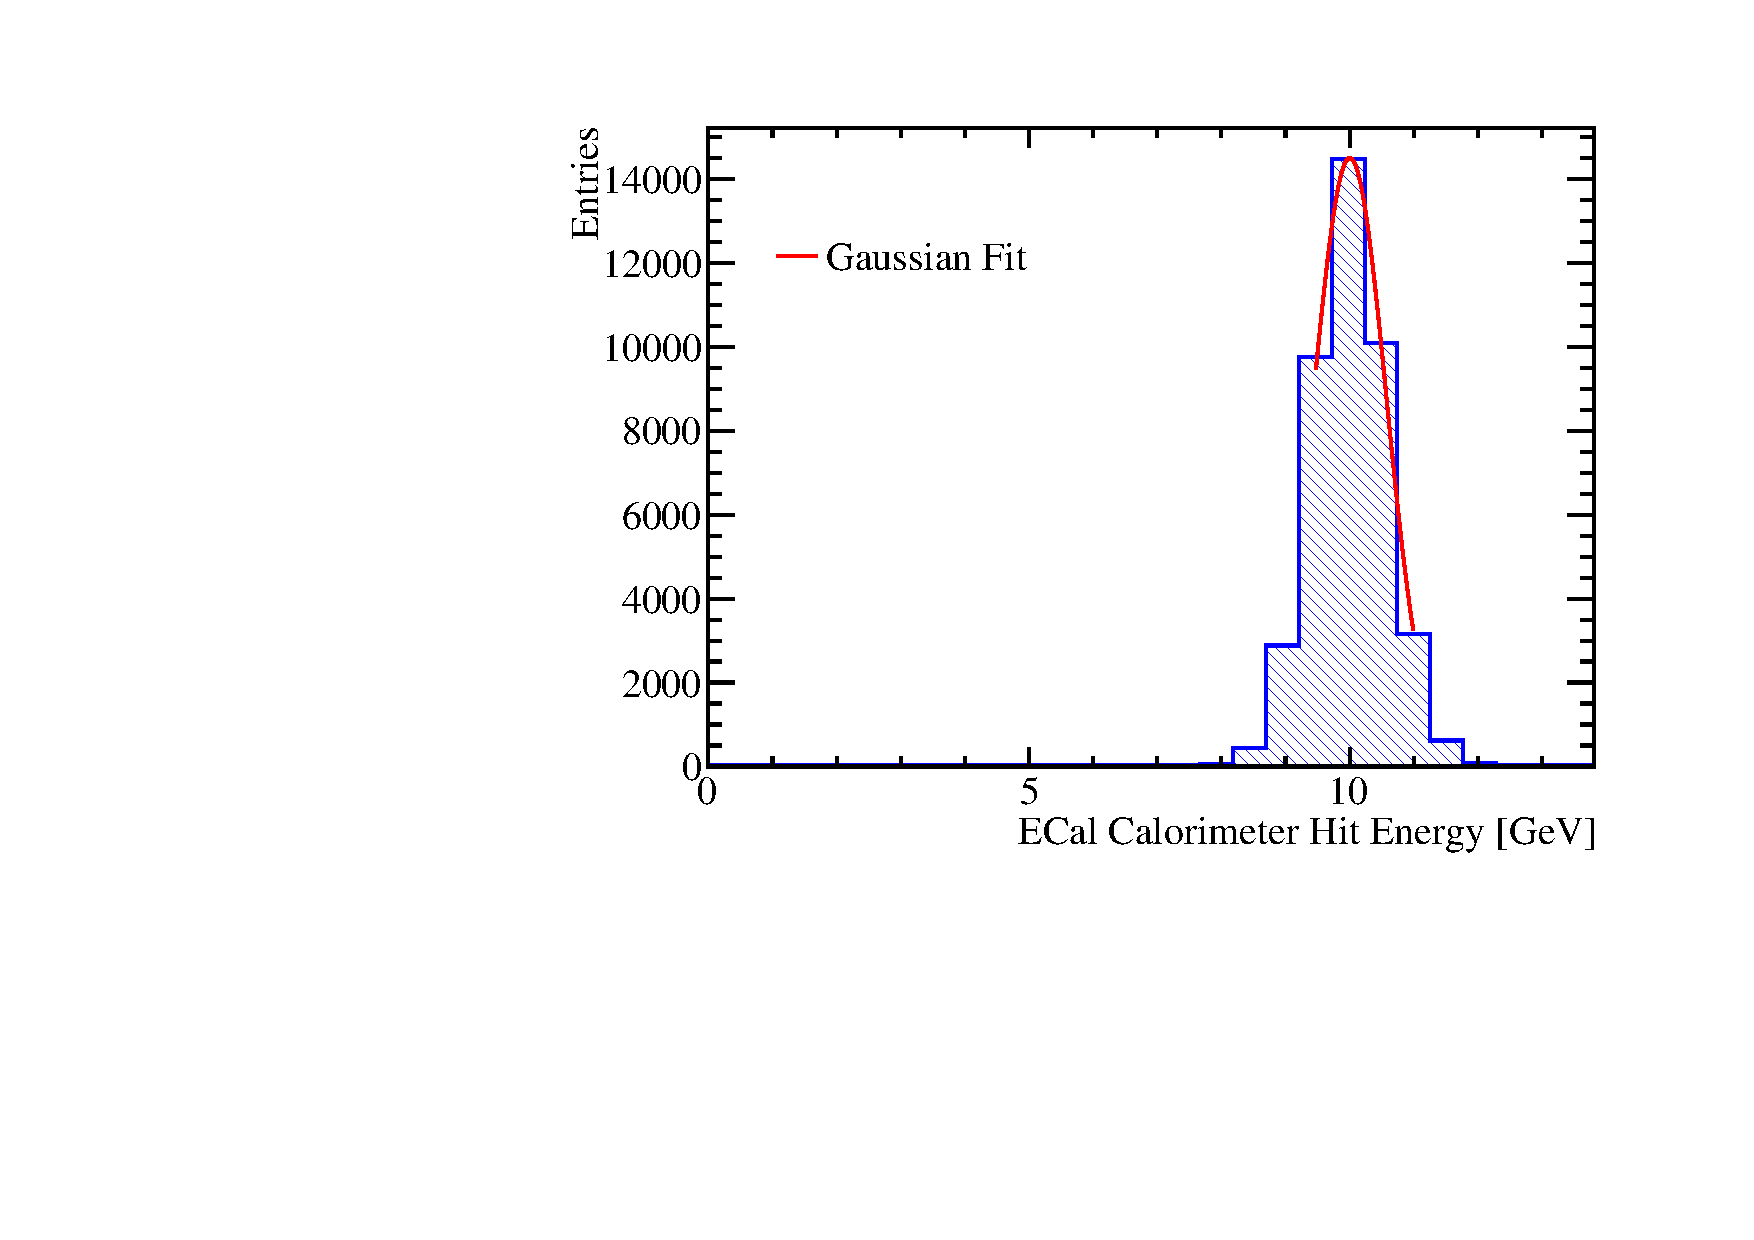
\includegraphics[width=0.5\textwidth]{EnergyEstimators/Plots/Calibration/Digitsation/ECal/DigitisationECalFit.pdf}
\caption[Gaussian fit to sum of the ECal calorimeter hit energies for 10 GeV $\gamma$ events with selection cuts.]{Gaussian fit to sum of the ECal calorimeter hit energies for 10 GeV $\gamma$ events with selection cuts.}
\label{fig:ecaldigifit}
\end{figure}

The calibration of the digitisation in the ECal is an iterative procedure and begins with the simulation of single $\gamma$ events using a trial calibration, with digitisation constant in the ECal $\alpha^{0}_{\text{ECal}}$ that may not be ideal.  Next the distribution of the sum of calorimeter hit energies within the ECal is produced for events passing the selection cuts, as shown in figure \ref{fig:ecaldigiselection}.  For an ideal calorimeter this distribution should be Gaussian, as was described in section CALORIMETER CHAPTER, therefore, a Gaussian fit is applied to this distribution and the mean, $E_{\text{Fit}}$, extracted.  To remove the effect of any outliers in this distribution, the fit is applied to the range of data with the smallest root mean square that contains at least 90 \% of the data.  An example of such a fit is shown in figure \ref{fig:ecaldigifit}.  In the case of ideal calibration the mean of this fit, $E_{\text{Fit}}$, would be equal $E_{MC}$.  It is assumed that any difference between the two is due to the calibration and to correct for this the digitisation constant from the trial calibration, $\alpha^{0}_{\text{ECal}}$, is rescaled by the ratio of the $E_{MC}$ to $E_{\text{Fit}}$.

\begin{equation}
\alpha^{0}_{\text{ECal}} \rightarrow \alpha_{\text{ECal}} = \alpha^{0}_{\text{ECal}} \times \frac{E_{MC}}{E_{Fit}}
\end{equation}

This procedure is then repeated until the $E_{\text{Fit}}$ falls within a specified tolerance.  The tolerance applied here was $|E_{\text{Fit}} - E_{\text{MC}}| < E_{\text{MC}} \times 5 \%$.  The binning used for the fitted histogram is chosen such that the bin width is equal to the desired tolerance on $E_{\text{Fit}}$ e.g. $E_{\text{MC}} \times 5 \% = 0.5$ GeV.  This tolerance is somewhat loose, however, it is tight enough to ensure successful application of PFA.  It should also be emphasised that the PFO energies used in downstream analyses have the electromagnetic and hadronic energy scale corrections applied, which are calibrated to a much tighter accuracy.

%========================================================================================

\subsubsection{HCal Digitisation}
\label{sec:hcaldigi}
The calibration for the digitisation in the HCal proceeds in a similar manor to that described for the ECal with a few key differences.  This calibration uses $K^{0}_{L}$ events at $E_{MC} = 20$ GeV as these neutral hadrons will deposit the bulk of their energy in the HCal.  The higher energy is used to create larger particle showers and sample deeper into the calorimeters.  

As in these events the $K^{0}_{L}$s have to pass through the ECal before arriving at the HCal and as the ECal contains $\approx 1 \lambda_{I}$, some of the $K^{0}_{L}$ begin showering in the ECal, as shown by figure \ref{fig:hcaldigikaonsplit}.  Such events are unsuitable for calibration of the HCal digitisation constants as rescaling $\alpha^{0}_{\text{HCal}}$ would not lead to a linear rescaling in $E_{\text{Fit}}$.  These events are vetoed in the even selections by applying selection cuts to ensure events used for the calibration deposit the bulk of their energy in the HCal.  

\begin{figure}
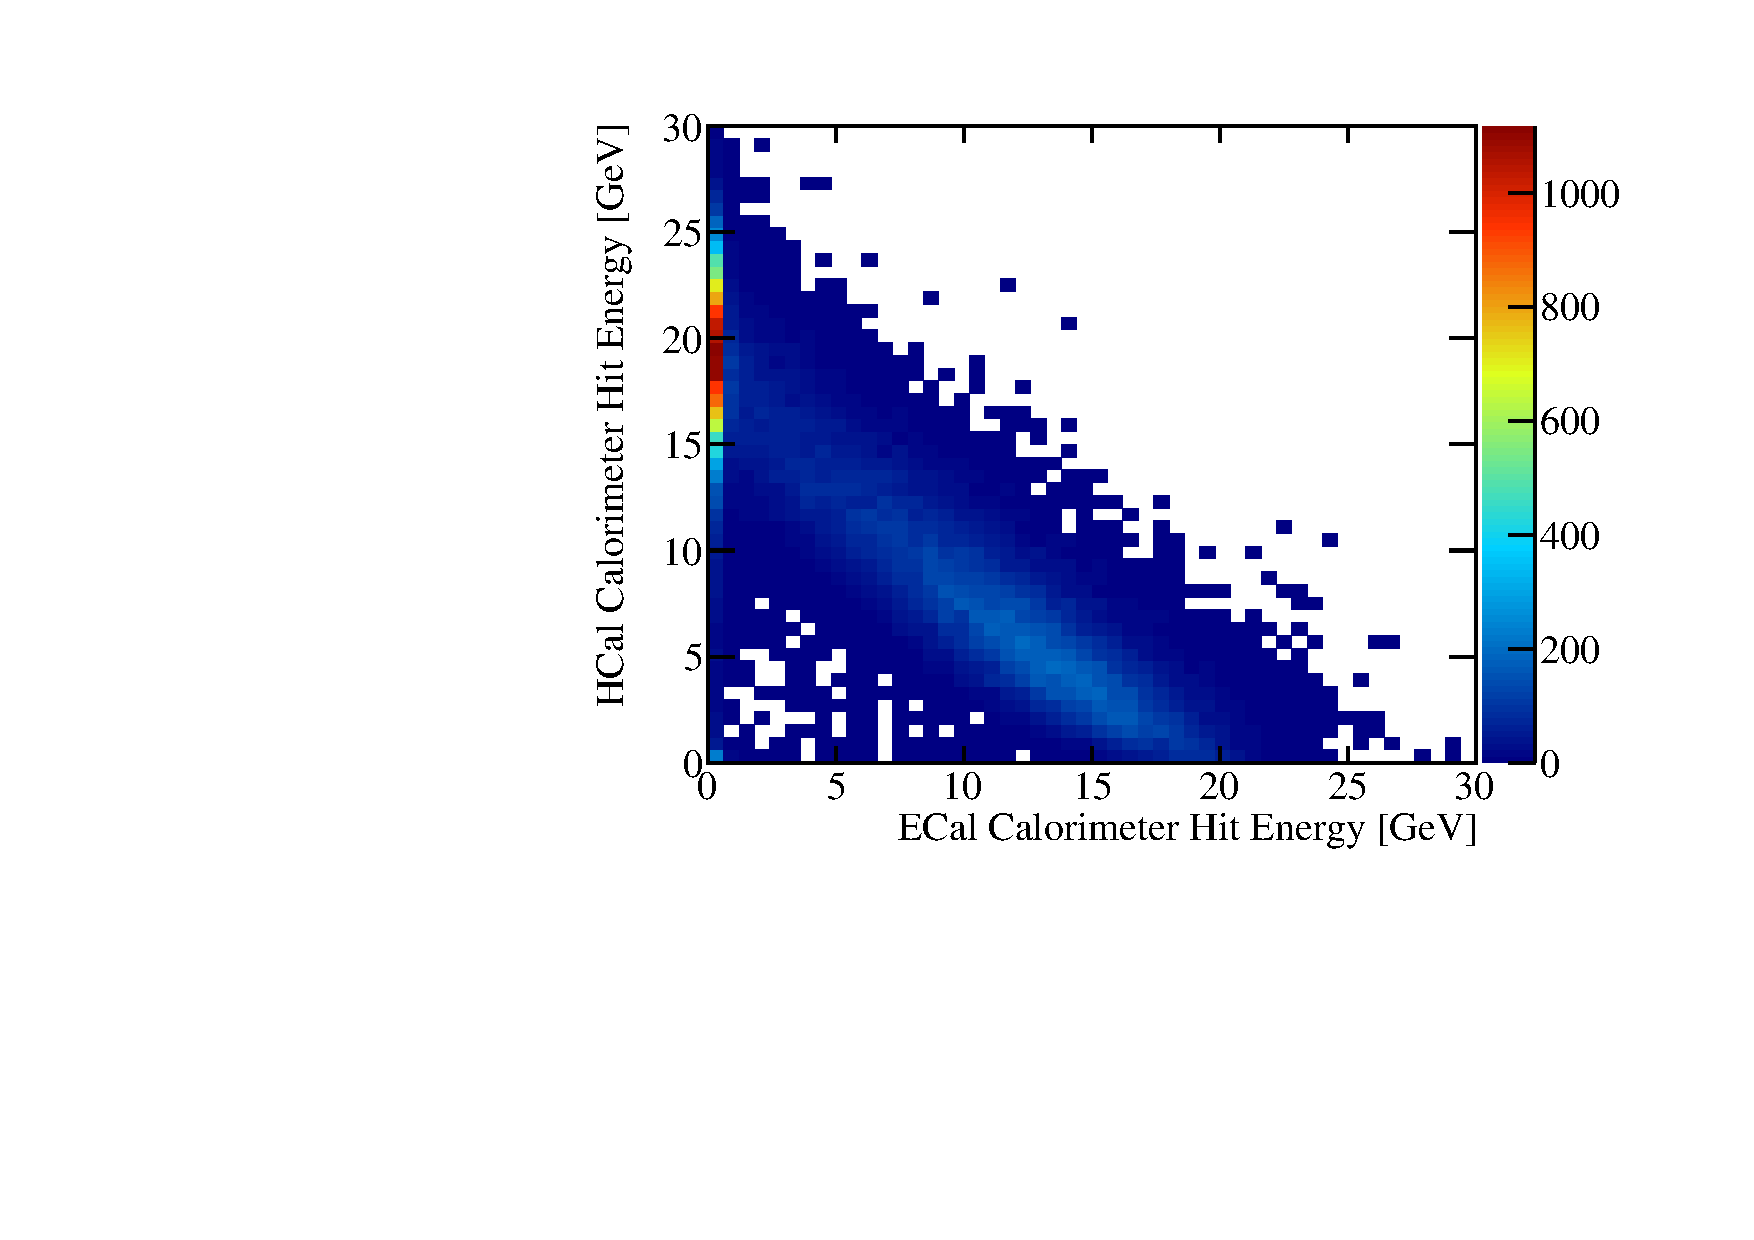
\includegraphics[width=0.5\textwidth]{EnergyEstimators/Plots/Calibration/Digitsation/HCal/ECalHCalKaon0LSplit.pdf}
\caption[Sum of calorimeter hit energies in ECal and HCal for 20 GeV $K^{0}_{L}$ events.]{Sum of calorimeter hit energies in ECal and HCal for 20 GeV $K^{0}_{L}$ events.}
\label{fig:hcaldigikaonsplit}
\end{figure}

Events are only considered in this analysis if a single neutral hadron PFO is reconstruction, the sum of any reconstructed energy found outside the HCal is less than 5\% of $E_{MC}$ and the last layer of the HCal where energy is deposited is in the first 90\% of the HCal.  The cut on the last HCal layer where energy is deposited is applied to veto events that shower late in the HCal and deposit a significant amount of energy in the uninstrumented coil region of the detector.  The impact of these cuts on the sum of HCal calorimeter hit energies for the $E_{MC} = 20$ GeV $K^{0}_{L}$ events is shown in figure \ref{fig:hcaldigiselection}.

\begin{figure}
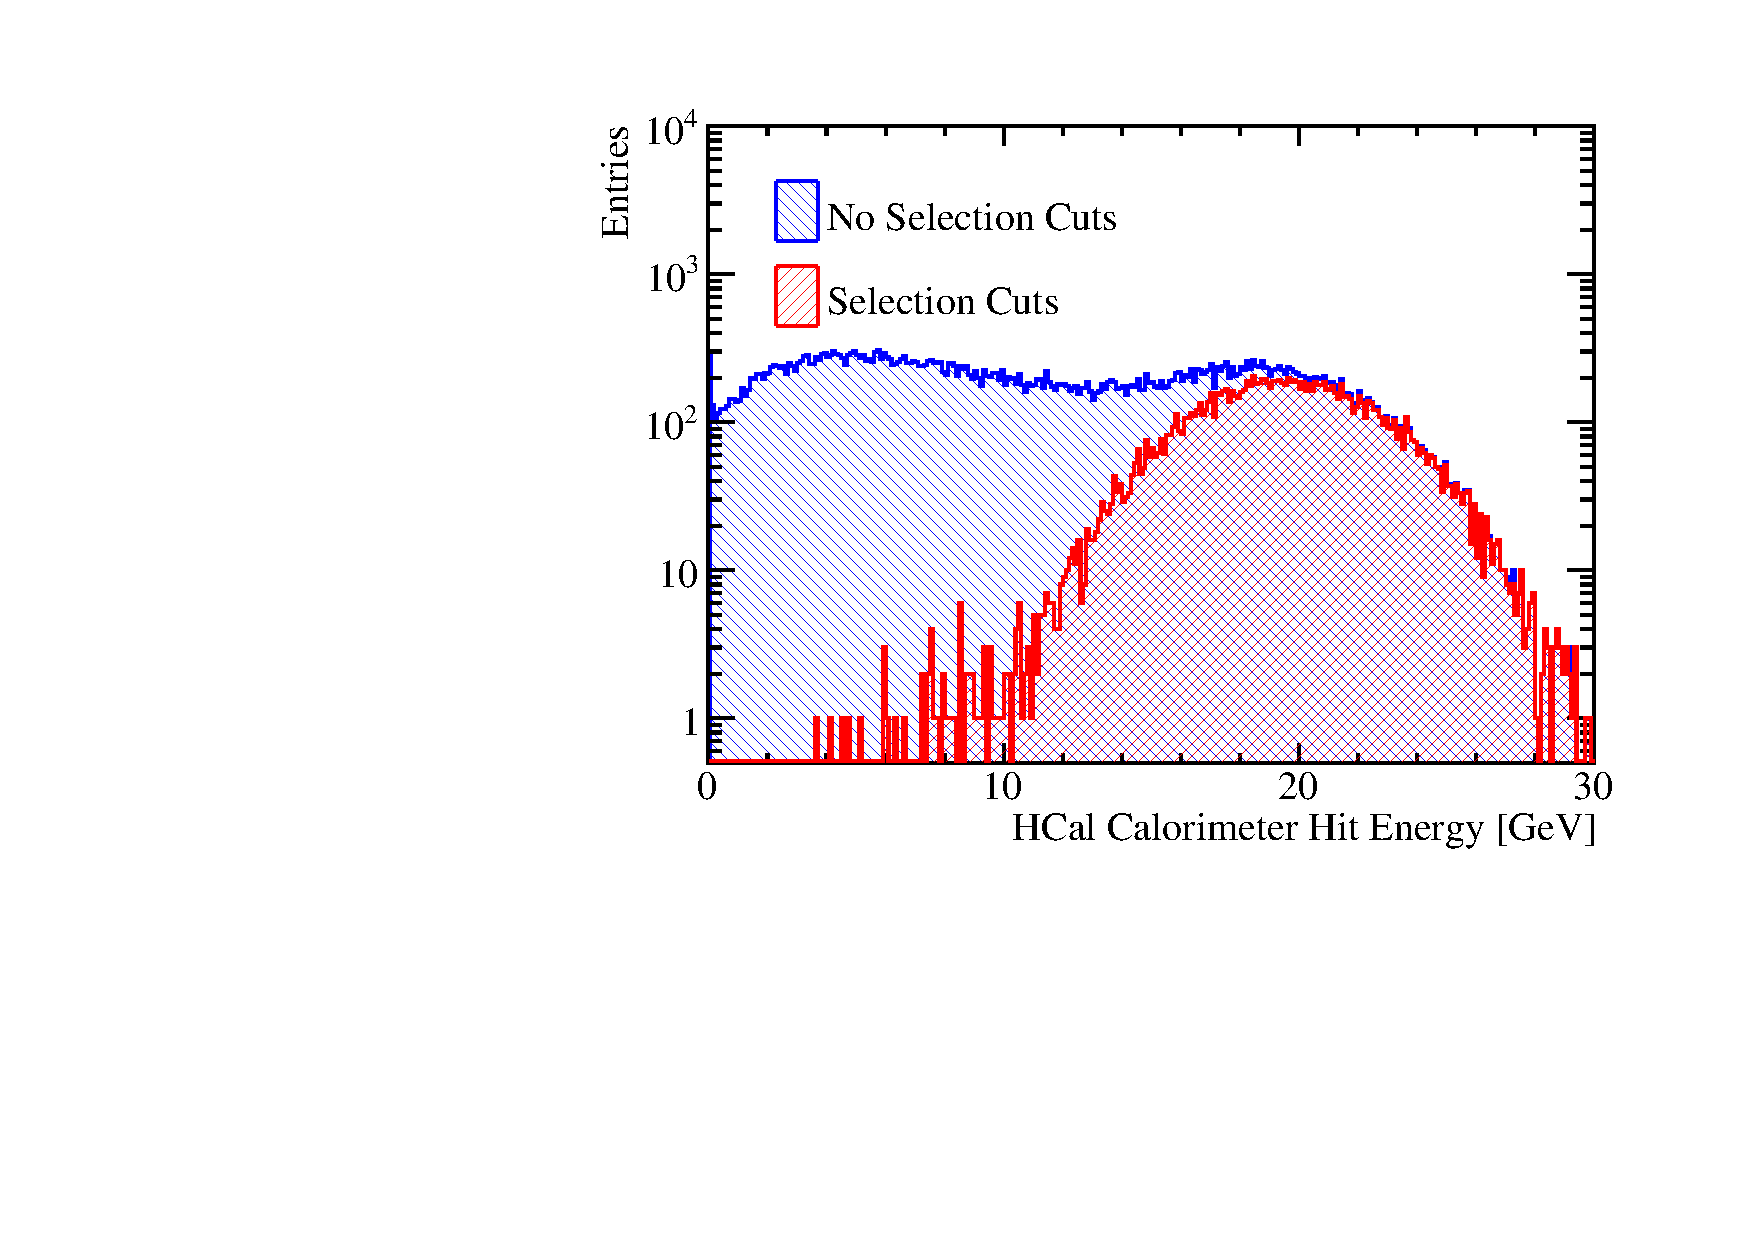
\includegraphics[width=0.5\textwidth]{EnergyEstimators/Plots/Calibration/Digitsation/HCal/DigitisationHCalSelection.pdf}
\caption[Sum of the HCal calorimeter hit energies for a 20 GeV $K^{0}_{L}$ events with and without the selection cuts.]{Sum of the HCal calorimeter hit energies for a 20 GeV $K^{0}_{L}$ events with and without the selection cuts.}
\label{fig:hcaldigiselection}
\end{figure}

There are two HCal digitisation constants used in the detector simulation, one applied for the Barrel and another for the EndCap.  This is to account for differences in hadronic shower dynamics between the two, such as differing magnetic field configurations in the Barrel and EndCap.  Both parameters are calibrated in the same manor, but have different cuts on $\theta$, the polar angle of the $K^{0}_{L}$.  For the Barrel region of the HCal events are selected if $0.2 < \text{cos}(\theta) < 0.6$, while for the EndCap events are selected if $0.8 < \text{cos}(\theta) < 0.9$.  These angular cuts are conservative to account for the transverse profile of the hadronic showers and ensure that they are confined to the relevant sub-detector.

Using these cuts the calibration procedure for the digitisation of the HCal Barrel and EndCap proceeds in the same manor as was described for the ECal, the details of which can be found in section \ref{sec:ecaldigi}.  Examples of the Gaussian fits applied to the sum of the calorimeter hit energies in the HCal Barrel and EndCap can be found in figure \ref{fig:hcaldigifit}.  

A noteworthy difference to the ECal digitisation procedure is that the target reconstructed energy for the $K^{0}_{L}$ samples is the kinetic energy as opposed to the total energy.  This decision was made as the majority of the neutral hadrons appearing in jets are neutrons and their accessible energy, what they can deposit in the detector, is their kinetic energy and not their rest mass energy.  This is the case as neutrons will come to a rest rather than decaying in the detector.  Therefore, calibrating to the kinetic energy should give the best performance for jet reconstruction.  

\begin{figure}
\subfloat[HCal Barrel.]{\label{fig:hcaldigibarrel}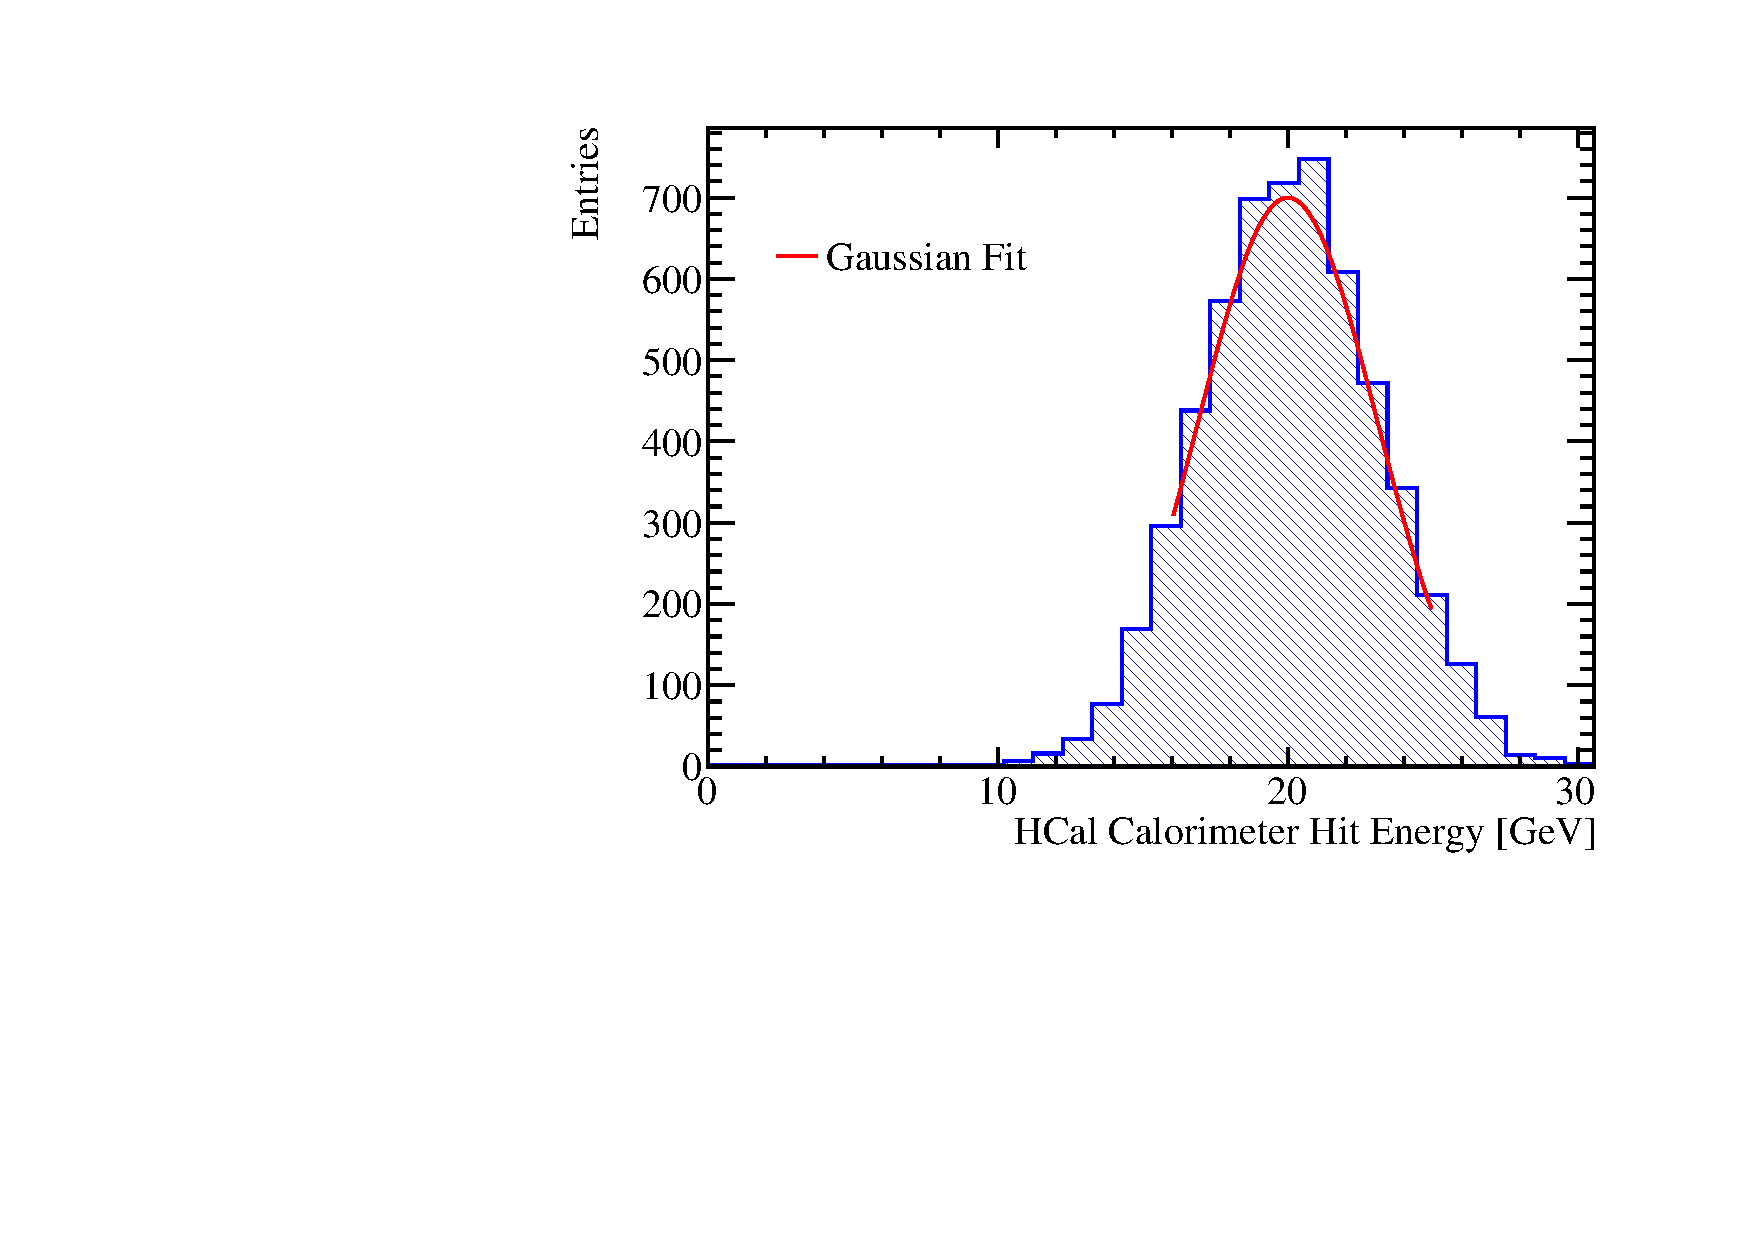
\includegraphics[width=0.5\textwidth]{EnergyEstimators/Plots/Calibration/Digitsation/HCal/DigitisationHCalBarrelFit.pdf}}
\subfloat[HCal EndCap.]{\label{fig:hcaldigiendcap}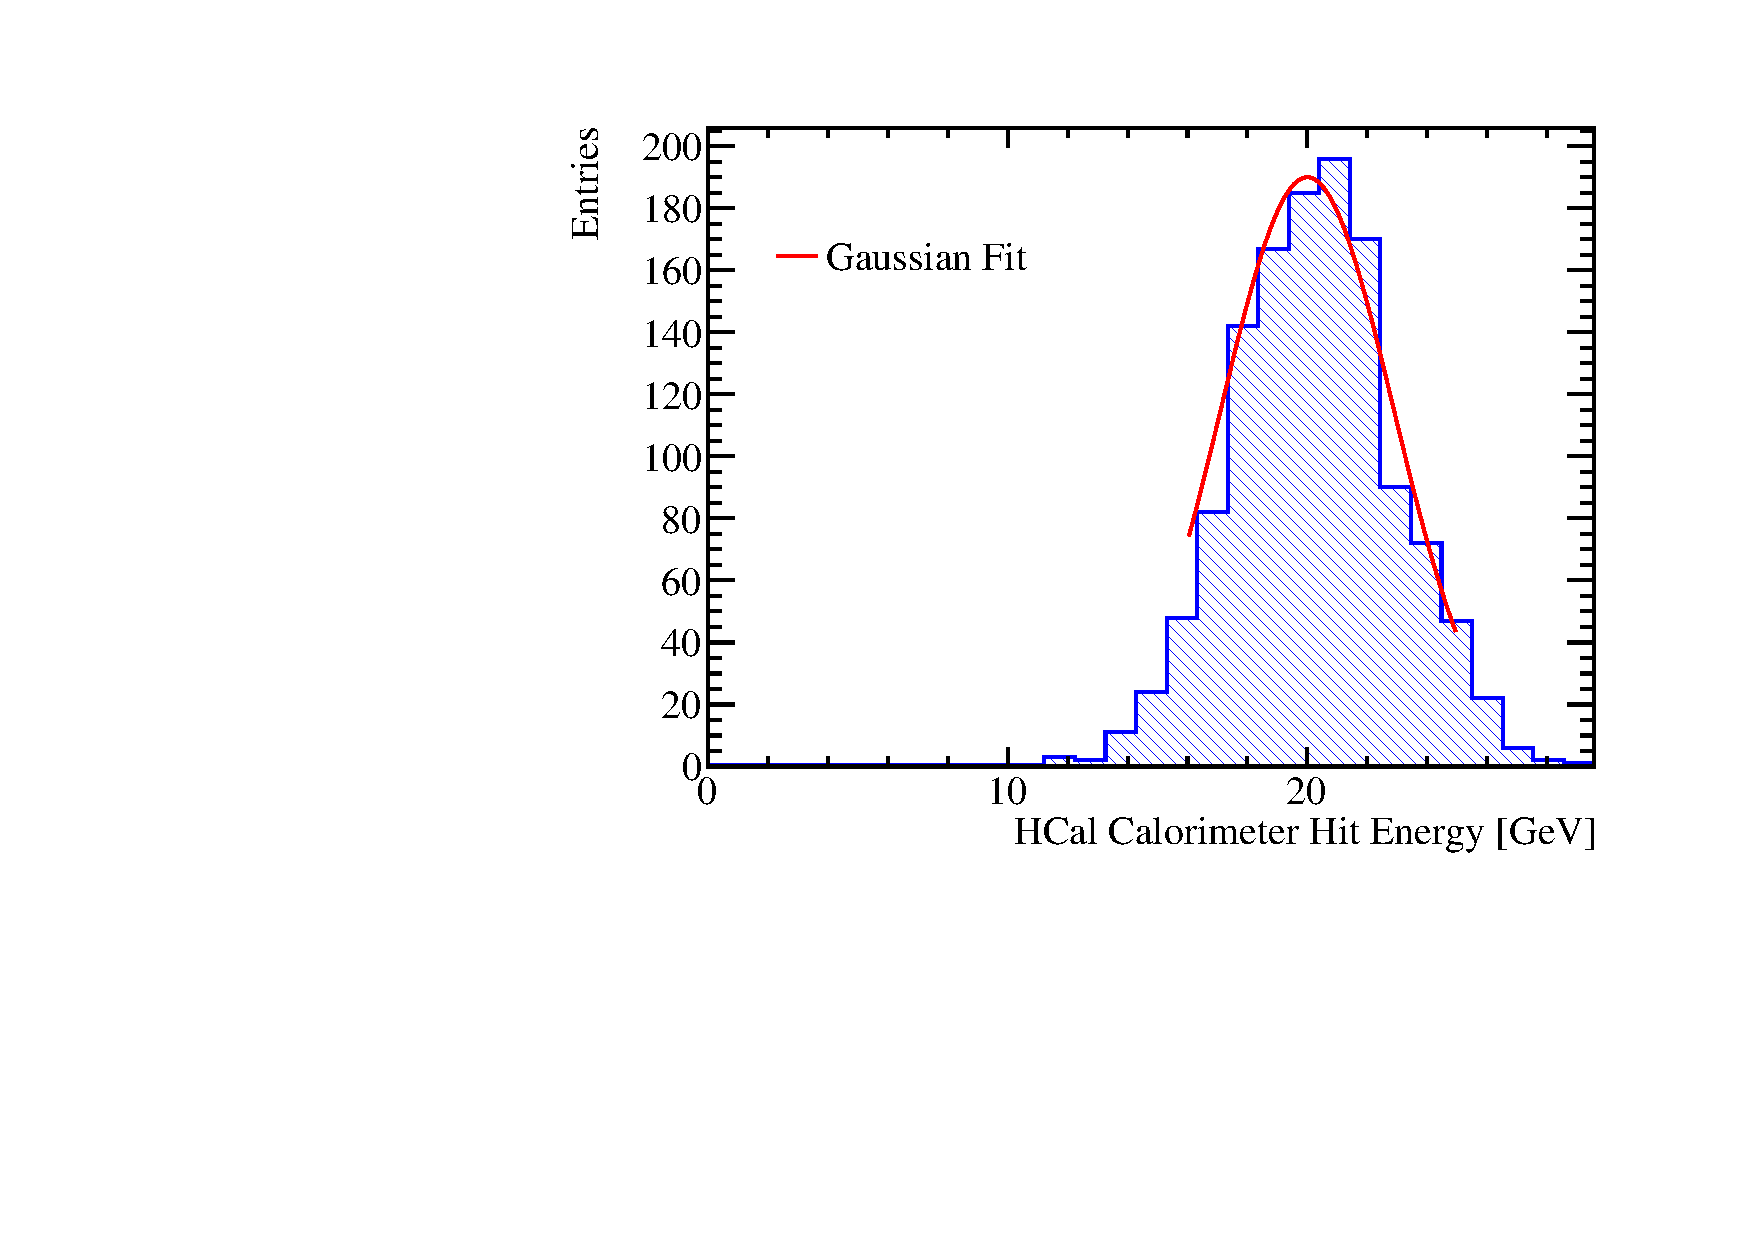
\includegraphics[width=0.5\textwidth]{EnergyEstimators/Plots/Calibration/Digitsation/HCal/DigitisationHCalEndCapFit.pdf}}
\caption[Gaussian fit to sum of the HCal calorimeter hit energies for 20 GeV $K^{0}_{L}$ events with selection cuts.]{Gaussian fit to sum of the HCal calorimeter hit energies for 20 GeV $K^{0}_{L}$ events with selection cuts.}
\label{fig:hcaldigifit}
\end{figure}

%========================================================================================

\subsubsection{HCal Ring Digitisation}
\label{sec:hcalringdigi}

\begin{figure}
\subfloat[]{\label{fig:ecal}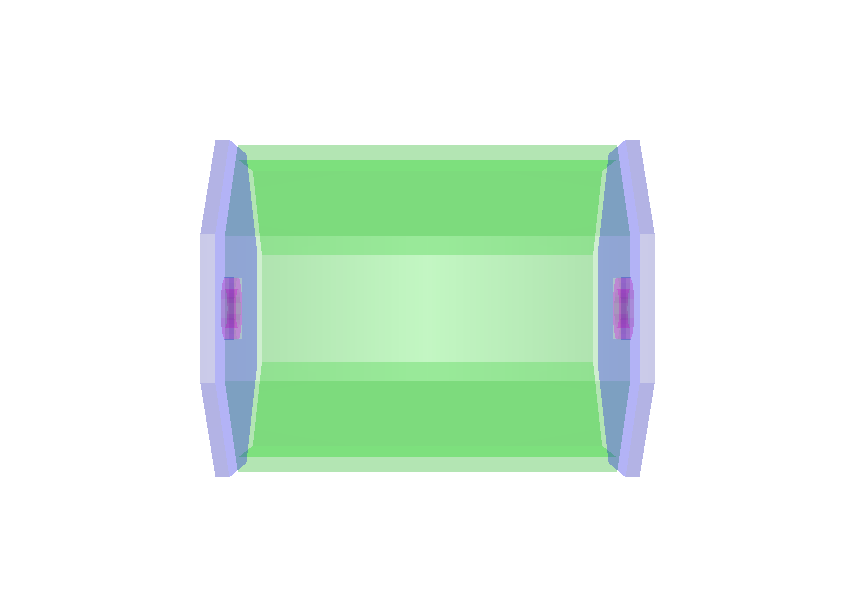
\includegraphics[width=0.33\textwidth]{EnergyEstimators/Plots/Calibration/VisualDisplay/ECal.png}}
\subfloat[]{\label{fig:hcal}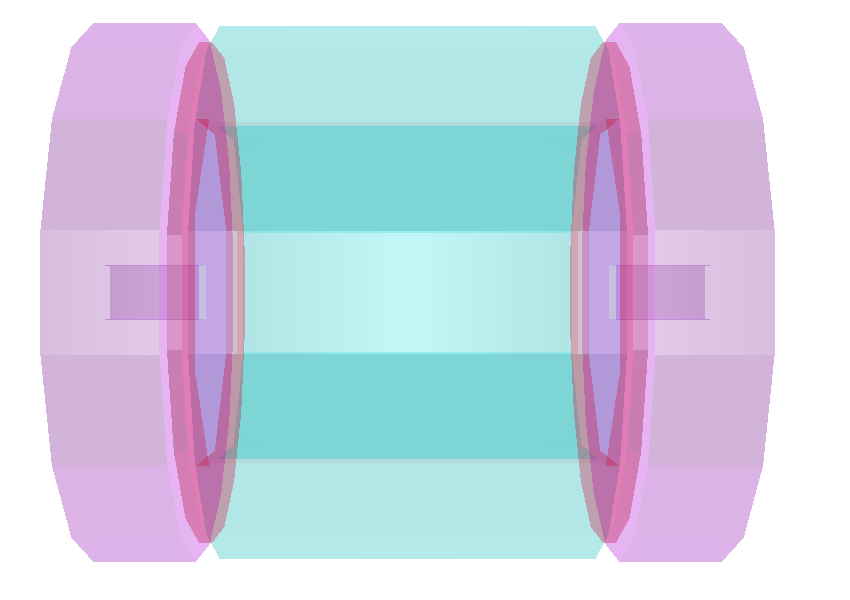
\includegraphics[width=0.33\textwidth]{EnergyEstimators/Plots/Calibration/VisualDisplay/HCal.png}}
\subfloat[]{\label{fig:hcalring}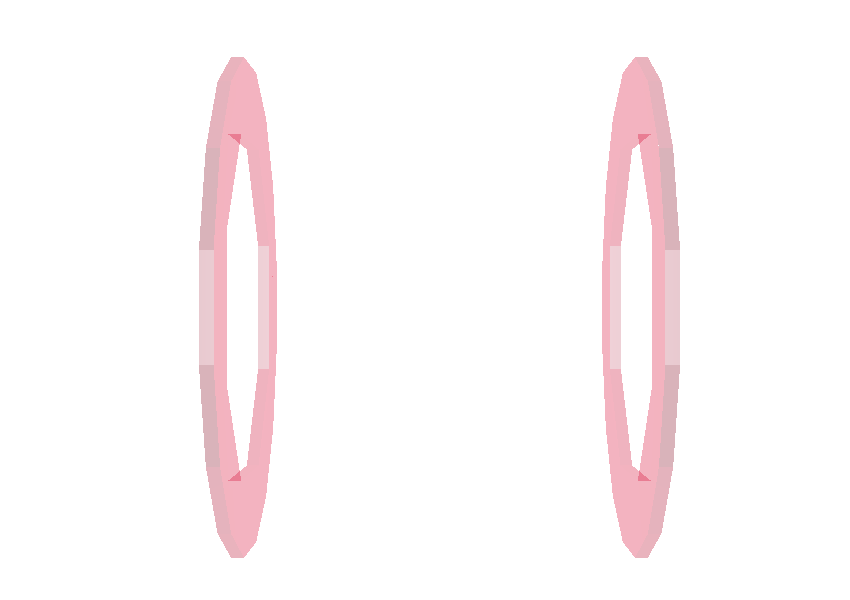
\includegraphics[width=0.33\textwidth]{EnergyEstimators/Plots/Calibration/VisualDisplay/HCalRing.png}}
\caption[A PandoraPFA event display showing the nominal ILD calorimeters.  \protect\subref{fig:ecal} show the ECal, \protect\subref{fig:hcal} shows the full HCal and \protect\subref{fig:hcalring} shows the HCal Ring.]{A PandoraPFA event display showing the nominal ILD calorimeters.  \protect\subref{fig:ecal} show the ECal, \protect\subref{fig:hcal} shows the full HCal and \protect\subref{fig:hcalring} shows the HCal Ring.}
\label{fig:calorimeters}
\end{figure}

The HCal Ring, illustrated in figure \ref{fig:calorimeters}, also has an independent digitisation constant to account for any difference in the hadronic shower development between the Ring, Barrel and EndCap.  The procedure used to calibrate this constant has to differs from that presented in section \ref{sec:hcaldigi} as it is unfeasible, due to the depth of the ring, to produce events that are wholly contained within it.  Fortunately, the size of the HCal ring means it plays a minimal role in the reconstruction, so precise calibration is not crucial.  To ensure that the calibration is approximately correct for the HCal Ring, $\alpha_{\text{HCal Ring}}$ is assumed to equal $\alpha_{\text{HCal EndCap}}$ multiplied by several factors designed to accounts for changes in the active layer thickness, absorber layer thickness and the MIP response between the HCal EndCap and Ring.  In detail:

\begin{equation}
\alpha_{\text{HCal Ring}} = \alpha_{\text{HCal EndCap}} \times \frac{\langle \text{cos}(\theta_\text{EndCap}) \rangle}{\langle \text{cos}(\theta_\text{Ring}) \rangle} \times \frac{P_\text{EndCap} }{P_\text{Ring} } \times \frac{L^{Absorber}_\text{EndCap}}{L^{Absorber}_\text{Ring} } \times \frac{L^{Active}_\text{Ring}}{L^{Active}_\text{EndCap}}
\end{equation}

where $\theta$ is the incident angle of the incoming particle to the calorimeter cells determined using the 20 GeV $K^{0}_{L}$ events, $L^{Active}$ is the active layer thickness and $L^{Absorber}$ is the absorber layer thickness. $P$ is the position of the MIP peak in the distribution of active layer cell energies, which has been corrected so that the MIP appears to enter the cell at normal incidence, and is determined using 10 GeV $\mu^{-}$ events.  Details on how $P$ is determined can be found in section \ref{sec:mipresponse}.

%========================================================================================

\subsection{MIP Scale Setting}
\label{sec:mipresponse}
The response of the various sub-detectors to a MIP has to be determined for both the digitisation processor and for PandoraPFA as both apply cuts in units of MIP response.  The digitiser applies cuts related to the electronic readout range of the various active layer technology options and applies a threshold on the minimum active layer energy for the creation of calorimeter hits.  PandoraPFA applies cuts designed to veto noise that would be present in a real detector.  Both these MIP responses, while intrinsically linked, have to be calculated separately as the digitiser requires the MIP peak definition from the active layer cell energies while, PandoraPFA requires the definition from the full cell, active and absorber layer, energies.  In these studies a MIP was defined as a 10 GeV $\mu^{-}$ \cite{Bichsel:2004ej} and no selection cuts applied to the sample.  

For the digitiser the MIP scale was defined as the, non-zero, peak in the distribution of the active layer calorimeter cell energies for normally incident $\mu^{-}$ as shown in figure \ref{fig:digitisermip}.  This distribution was produced using a sample of $\mu^{-}$ events that are spatially isotropic about the impact point.  A direction correction factor, $\text{cos}(\theta)$ where $\theta$ is the incident angle of the incoming $\mu^{-}$ to the calorimeter cell, was applied to the active layer cell energies to generate the effect of having normally incident $\mu^{-}$.  

\begin{figure}
\subfloat[ECal.]{\label{fig:digitisermipecal}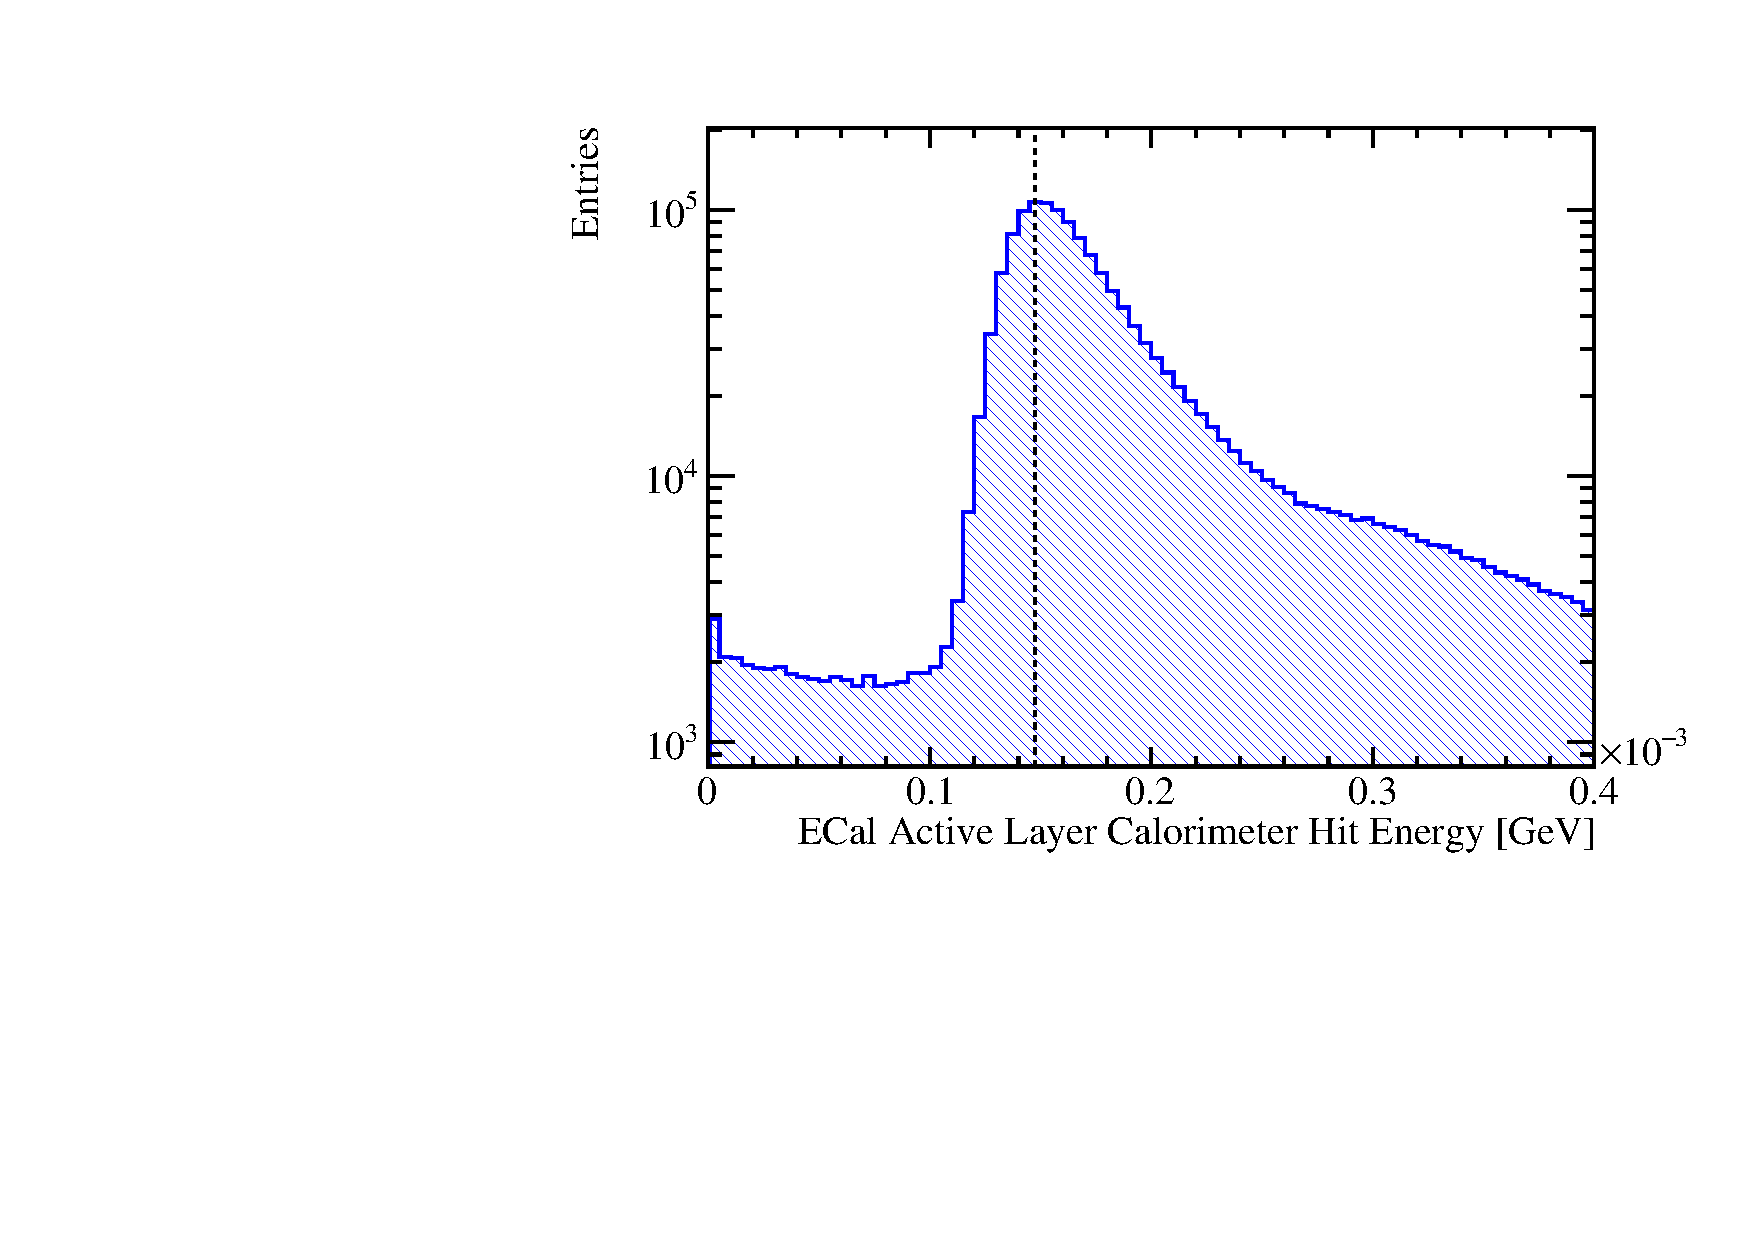
\includegraphics[width=0.5\textwidth]{EnergyEstimators/Plots/Calibration/MIPScale/Digitiser/MIPScaleDigitiserECal.pdf}}
\subfloat[HCal Barrel.]{\label{fig:digitisermiphcalbarrel}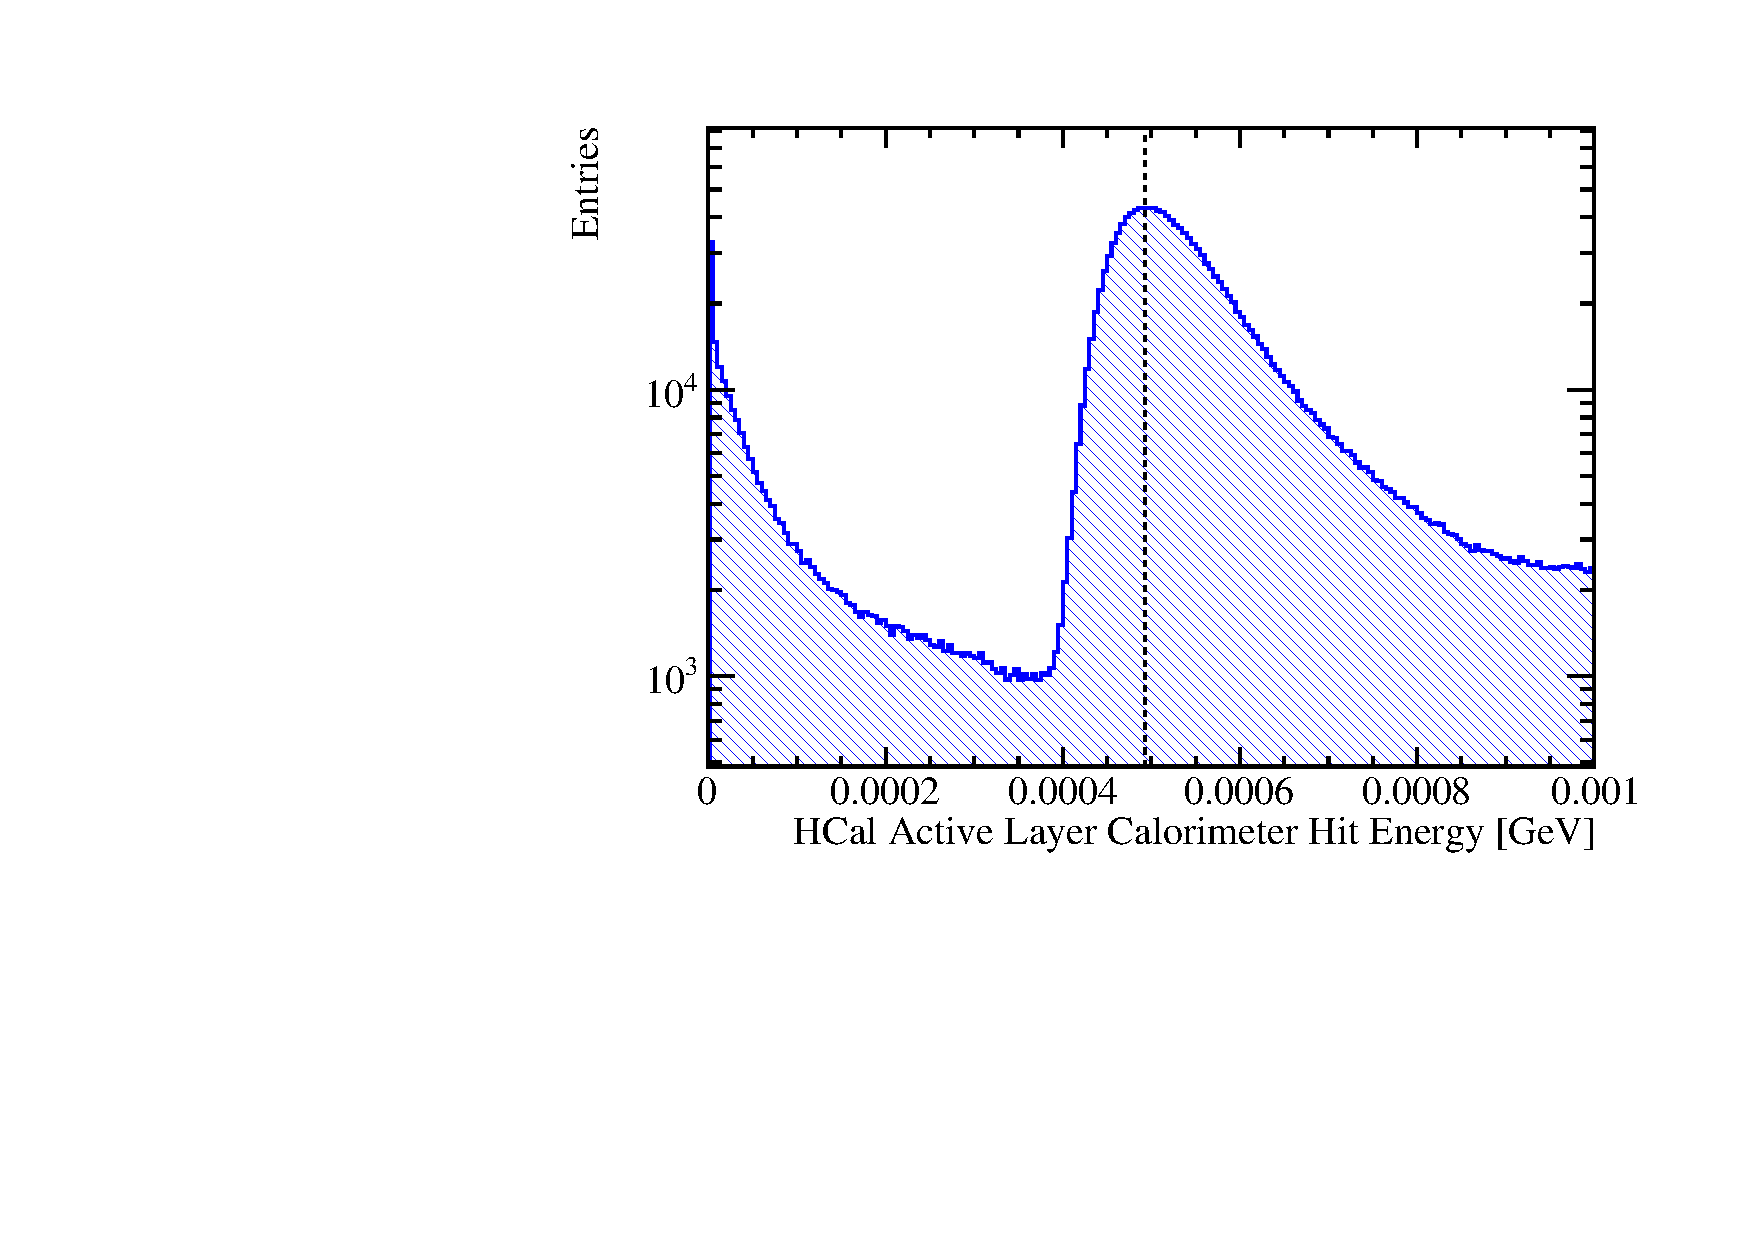
\includegraphics[width=0.5\textwidth]{EnergyEstimators/Plots/Calibration/MIPScale/Digitiser/MIPScaleDigitiserHCalBarrel.pdf}} \\
\subfloat[HCal EndCap.]{\label{fig:digitisermiphcalendcap}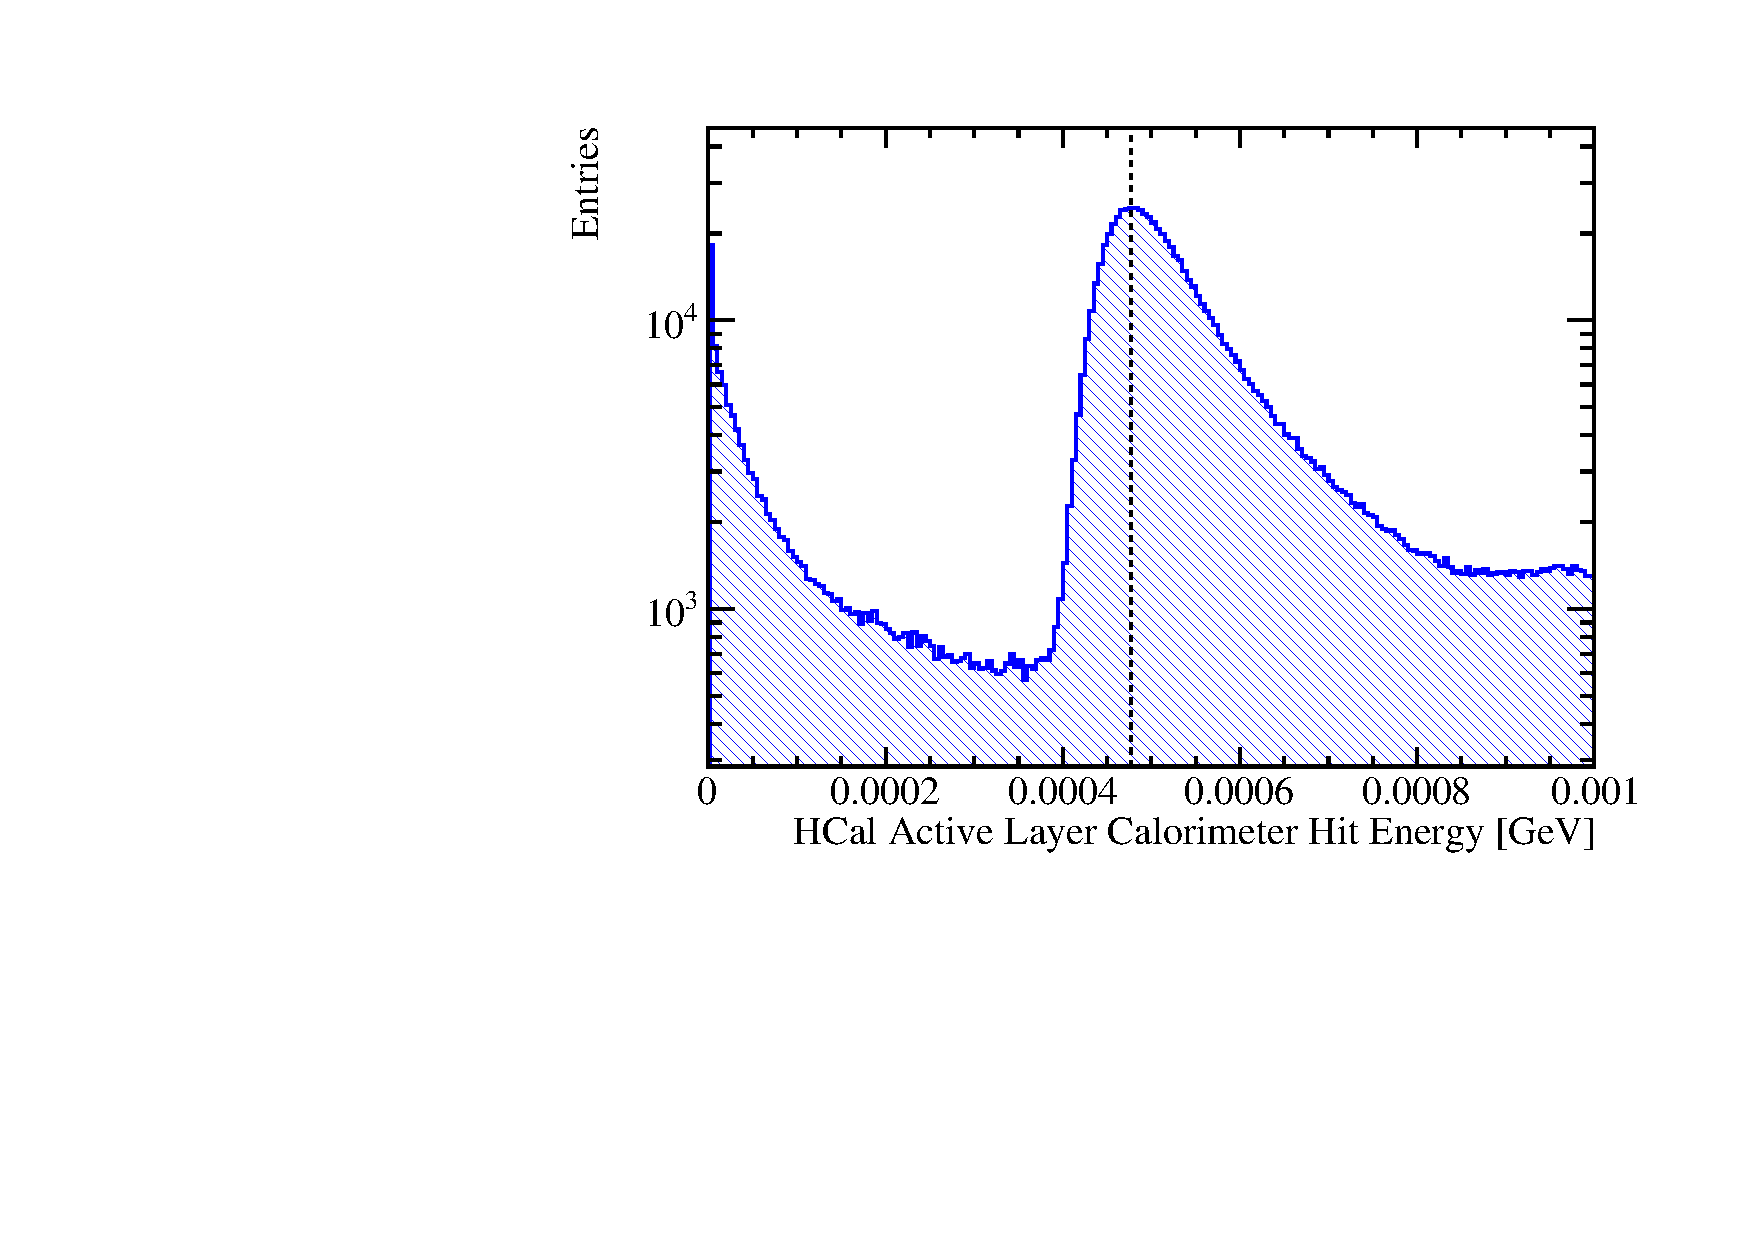
\includegraphics[width=0.5\textwidth]{EnergyEstimators/Plots/Calibration/MIPScale/Digitiser/MIPScaleDigitiserHCalEndCap.pdf}}
\subfloat[HCal Ring.]{\label{fig:digitisermiphcalring}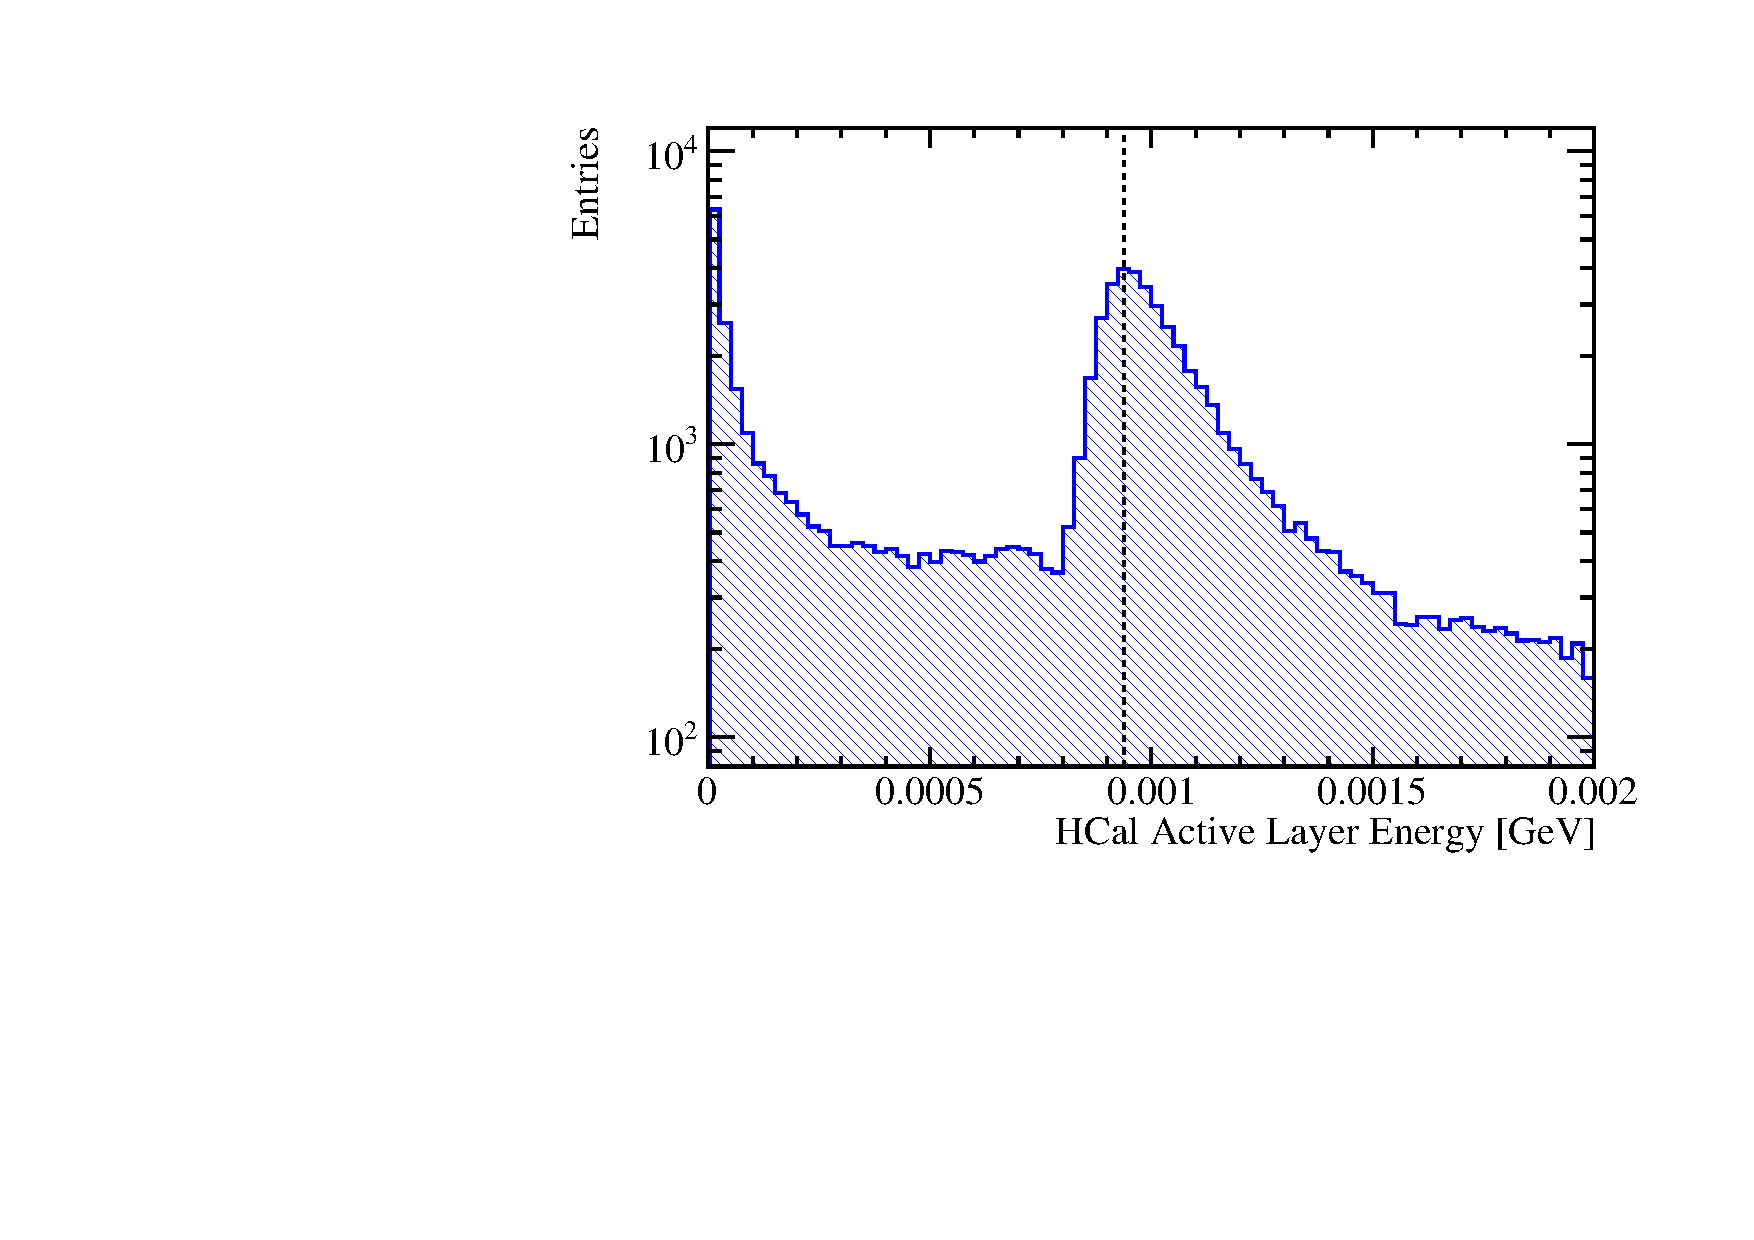
\includegraphics[width=0.5\textwidth]{EnergyEstimators/Plots/Calibration/MIPScale/Digitiser/MIPScaleDigitiserHCalOther.pdf}}
\caption[The active layer calorimeter cell energy distributions for \protect\subref{fig:digitisermipecal} the ECal, \protect\subref{fig:digitisermiphcalbarrel} the HCal Barrel, \protect\subref{fig:digitisermiphcalendcap} the HCal EndCap and \protect\subref{fig:digitisermiphcalring} the HCal Ring for 10 GeV $\mu^{-}$ events.]{The active layer calorimeter cell energy distributions for \protect\subref{fig:digitisermipecal} the ECal, \protect\subref{fig:digitisermiphcalbarrel} the HCal Barrel, \protect\subref{fig:digitisermiphcalendcap} the HCal EndCap and \protect\subref{fig:digitisermiphcalring} the HCal Ring for 10 GeV $\mu^{-}$ events.}
\label{fig:digitisermip}
\end{figure}

In the digitiser processor a single value for the MIP peak was required for the HCal and that was taken as the MIP peak position for the HCal Barrel.  The MIP peaks were separately calculated for the HCal EndCap and Ring for the purposes of the HCal Ring digitisation described in section \ref{sec:hcalringdigi}.  The realistic digitisation features present in the simulation of the ECal and HCal are not available for the muon chamber simulation, therefore, no MIP peak setting for that digitisation step is required.

A similar procedure was employed for calculation of the MIP peak in PandoraPFA.  One important difference was the distribution used for setting the MIP scale in PandoraPFA is the distribution of calorimeter cell energies, i.e. the energy in the active and absorber layers of a cell, and not just the active layer energies.  Examples of the distributions used to set the MIP scale in PandoraPFA can be found in figure \ref{fig:pandoramip}.  There are few populated low calorimeter cell energy bins due to cuts applied in the digitiser on the minimum active layer energy required to make a calorimeter hit.  The double peak structure in the ECal calorimeter hit energy distribution is present due to the doubling of the thickness of the ECal absorber material, from 2.1 mm to 4.2 mm tungsten, in the ILD detector model that occurs for the back 10 layers of the 30 layer ECal.  Further differences between the MIP scale setting in the digitiser and PandoraPFA worthy of note are that in PandoraPFA the HCal MIP scale setting combines the HCal sub-detectors, the Barrel, EndCal and Ring, together and PandoraPFA requires the MIP scale to be set in the muon chamber, which requires the muon chamber cell energy distribution to be created.  

\begin{figure}
\subfloat[]{\label{fig:pandoramipecal}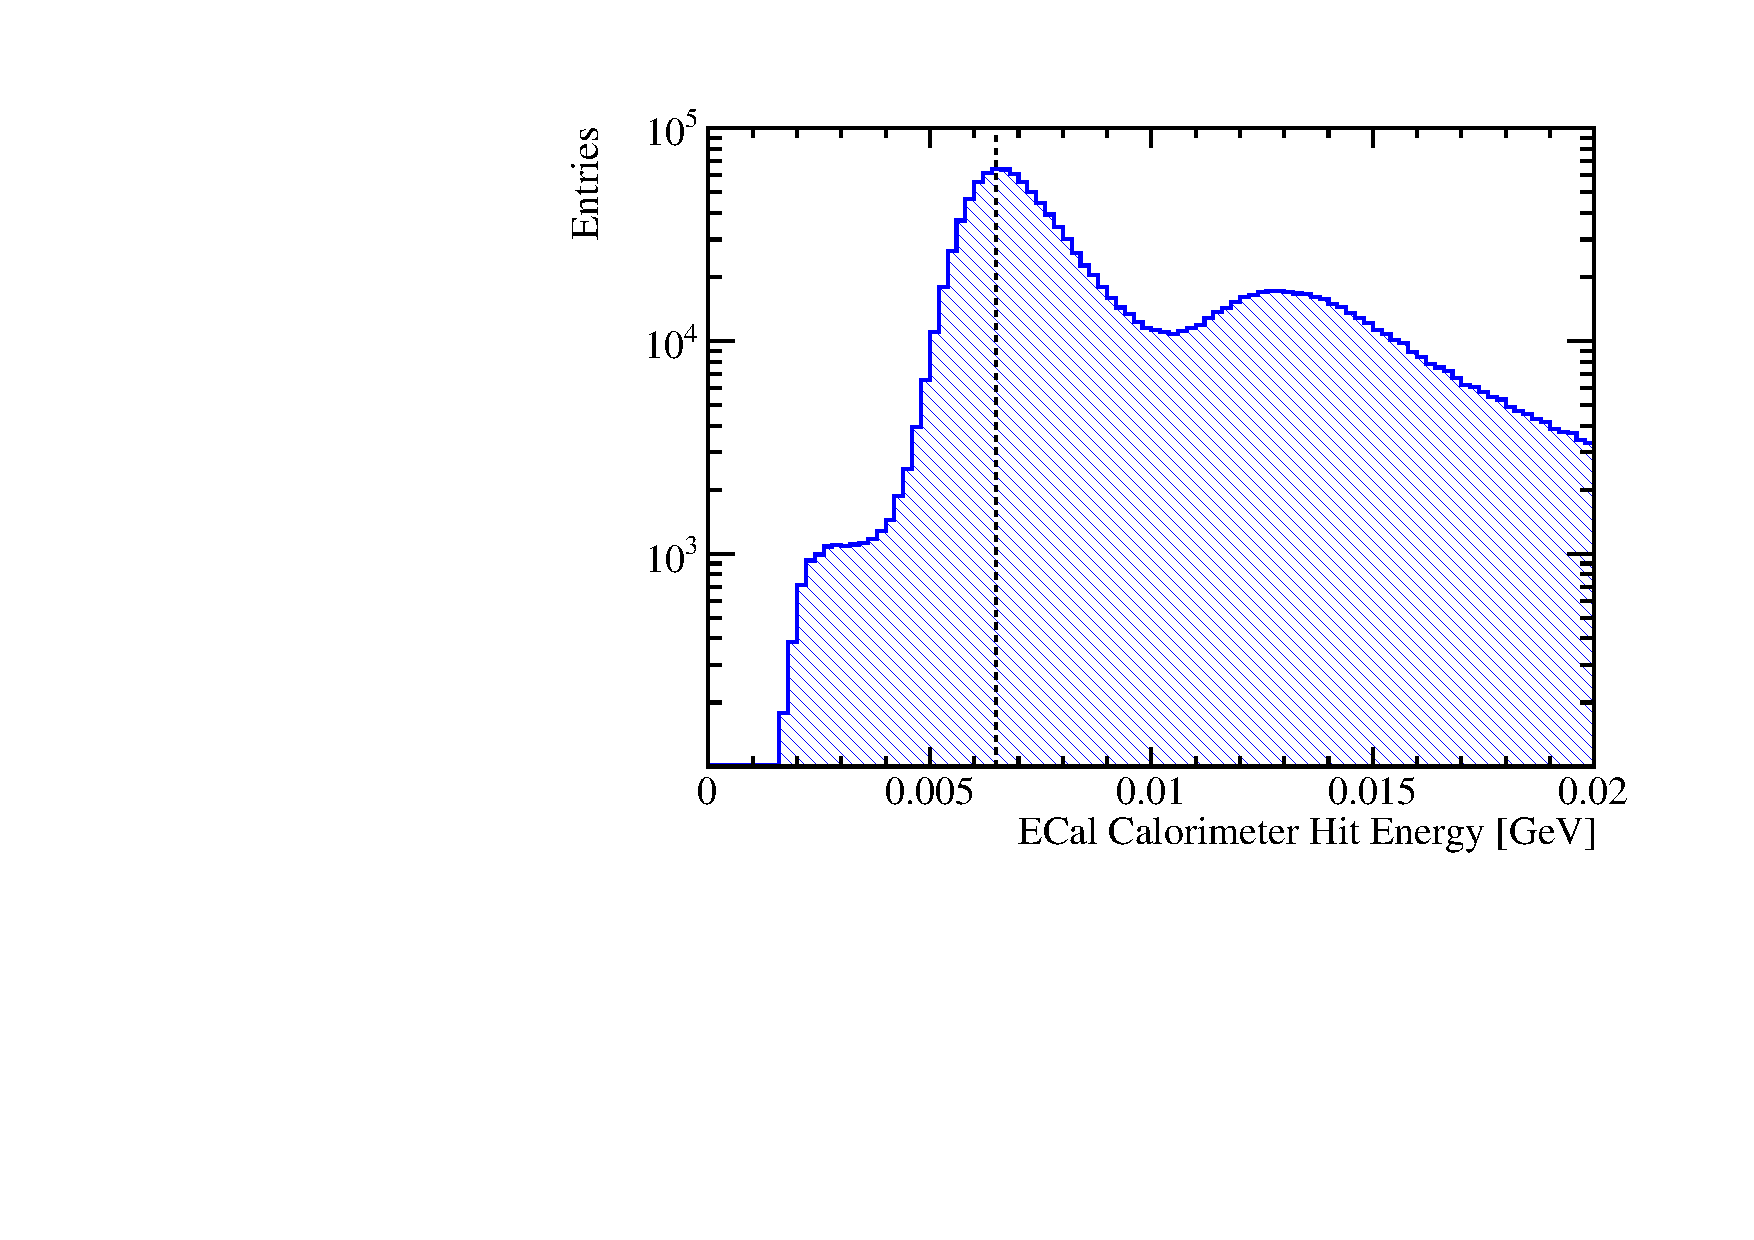
\includegraphics[width=0.5\textwidth]{EnergyEstimators/Plots/Calibration/MIPScale/PandoraPFA/MIPScalePandoraPFAECal.pdf}}
\subfloat[]{\label{fig:pandoramiphcal}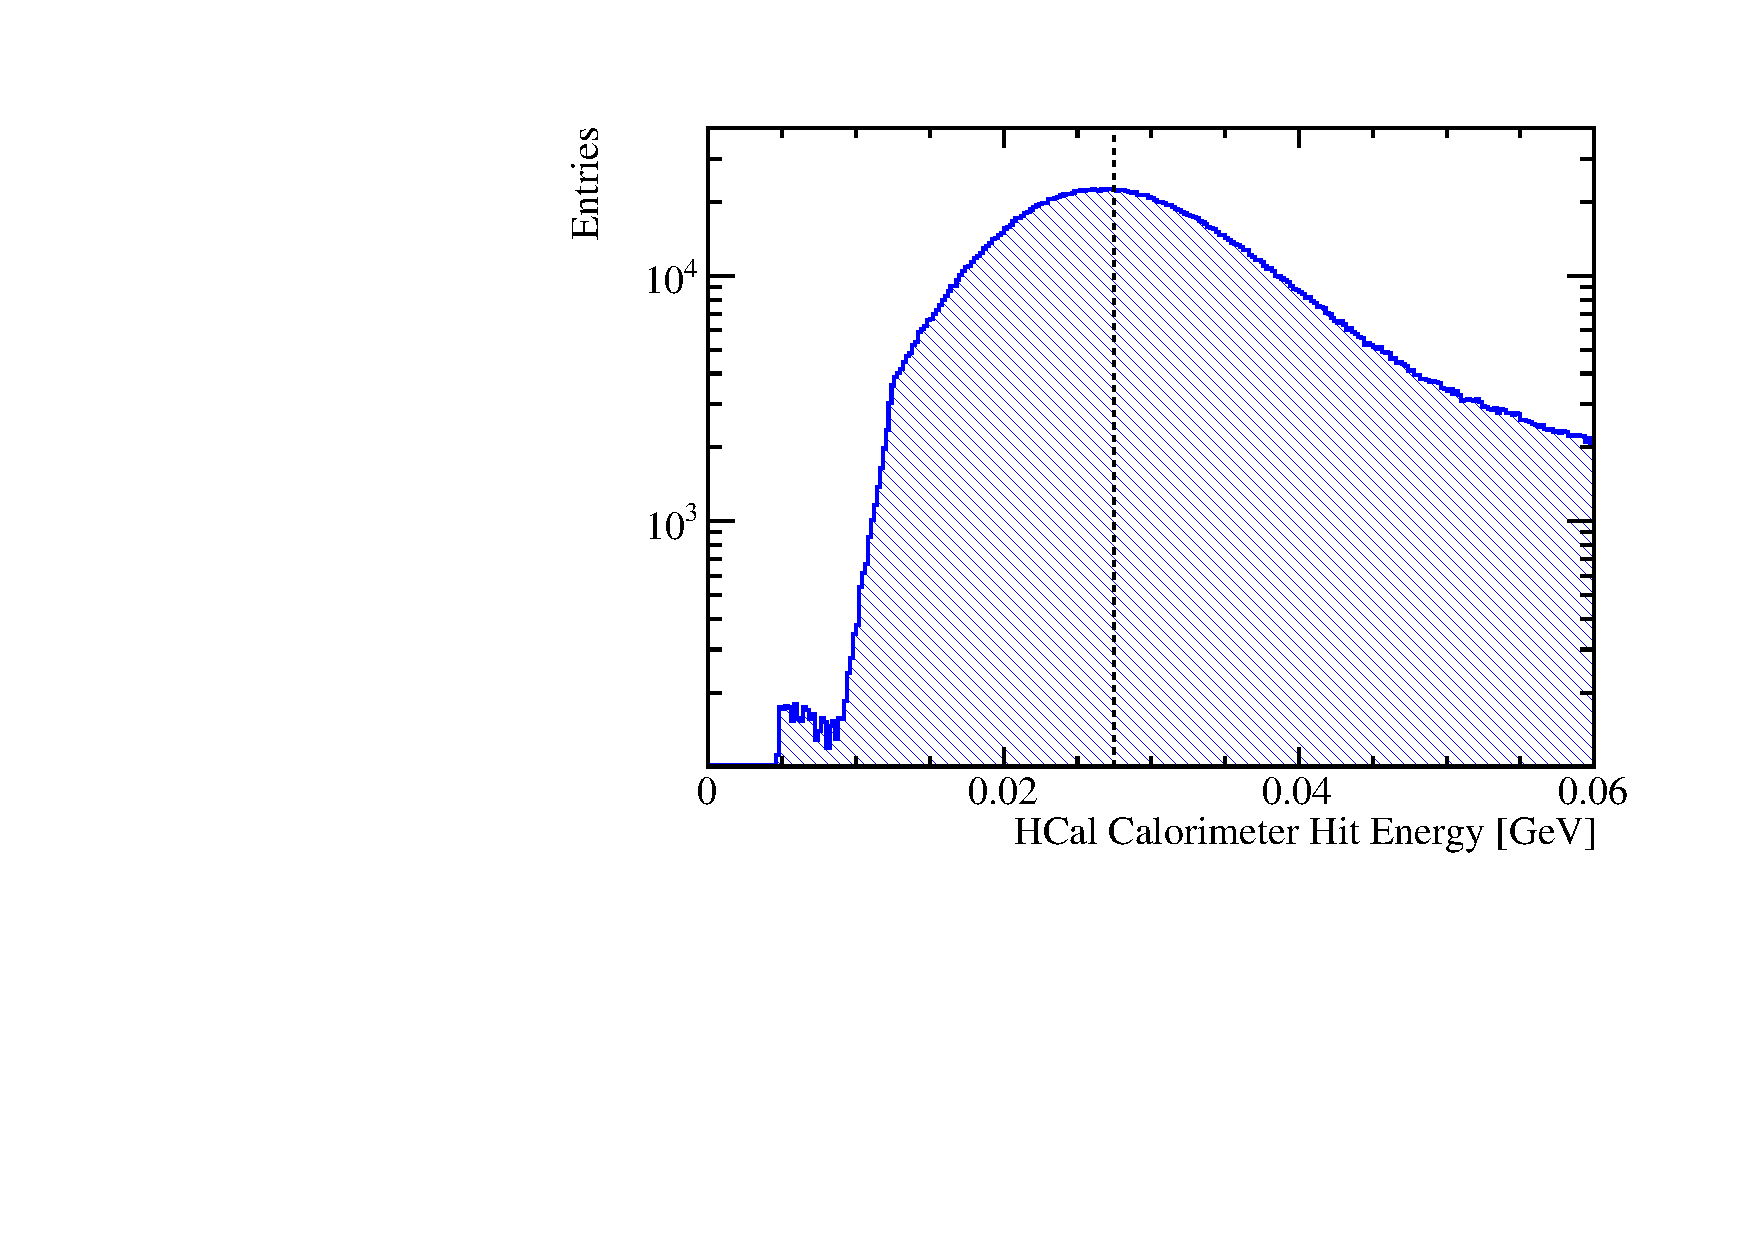
\includegraphics[width=0.5\textwidth]{EnergyEstimators/Plots/Calibration/MIPScale/PandoraPFA/MIPScalePandoraPFAHCal.pdf}} \\
\subfloat[]{\label{fig:pandoramipmuon}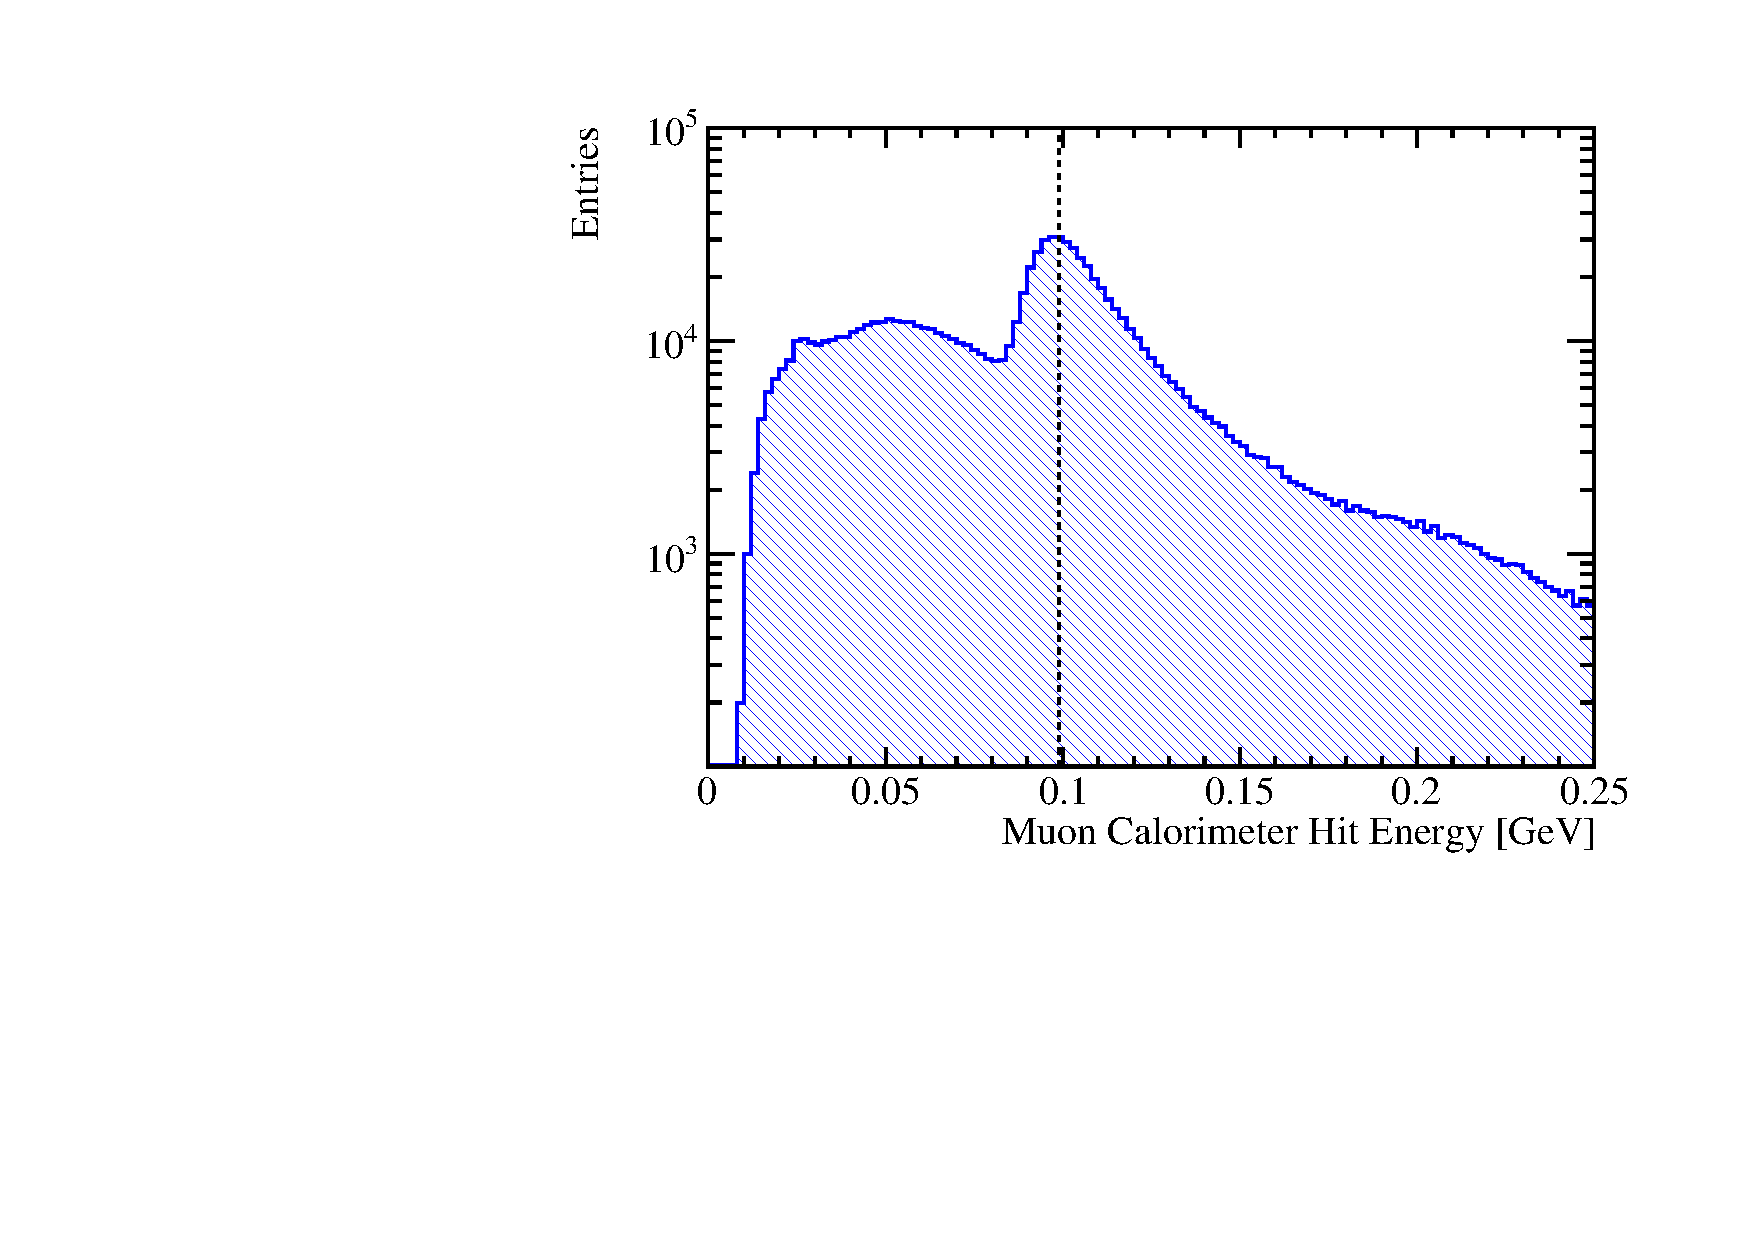
\includegraphics[width=0.5\textwidth]{EnergyEstimators/Plots/Calibration/MIPScale/PandoraPFA/MIPScalePandoraPFAMuon.pdf}}
\caption[The calorimeter cell energy distributions for \protect\subref{fig:pandoramipecal} the ECal, \protect\subref{fig:pandoramiphcal} the HCal and \protect\subref{fig:pandoramipmuon} the muon chamber for 10 GeV $\mu^{-}$ events.]{The calorimeter cell energy distributions for \protect\subref{fig:pandoramipecal} the ECal, \protect\subref{fig:pandoramiphcal} the HCal and \protect\subref{fig:pandoramipmuon} the muon chamber for 10 GeV $\mu^{-}$ events.}
\label{fig:pandoramip}
\end{figure}

%========================================================================================

\subsection{Electromagnetic and hadronic scale setting}
\label{sec:scalesetting}
The electromagnetic and hadronic scales have to be independently set in the simulation to account for the different mechanisms governing the propagation of electromagnetic and hadronic showers.  The setting of the scales involves tuning four parameters in PandoraPFA that correspond to energy rescaling factors, which are applied to energy measurements from electromagnetic and hadronic showering particles in the ECal and HCal.  

%========================================================================================

\subsubsection{Electromagnetic scale setting}
\label{sec:emscalesetting}
The electromagnetic scale in the ECal, $\beta^{EM}_{ECal}$, is determined using $\gamma$ events at $E_{MC} = 10$ GeV.  $\gamma$ events are ideal for the setting of the electromagnetic scale as they procedure electromagnetic showers and are primarily confined to the ECal at the energy considered, which was shown in figure \ref{fig:ecaldigiphotonsplit}.  

Cuts are applied to ensure that only events where the bulk of the energy is deposited within the ECal are used for this part of the calibration.  Less than 1\% of the reconstructed energy is outside the ECal to ensure the event is contained.  Furthermore, cuts requiring a single $\gamma$ be reconstructed are added to veto pattern recognition failures.  $\gamma$ conversions are excluded at MC level to ensure energy measurements used in the calibration arise from the calorimeters and not the charged particle tracks.  The impact of these cuts on the electromagnetic energy measured in the ECal for 10 GeV $\gamma$ events is shown in figure \ref{fig:ecalemscaleselection}.

\begin{figure}
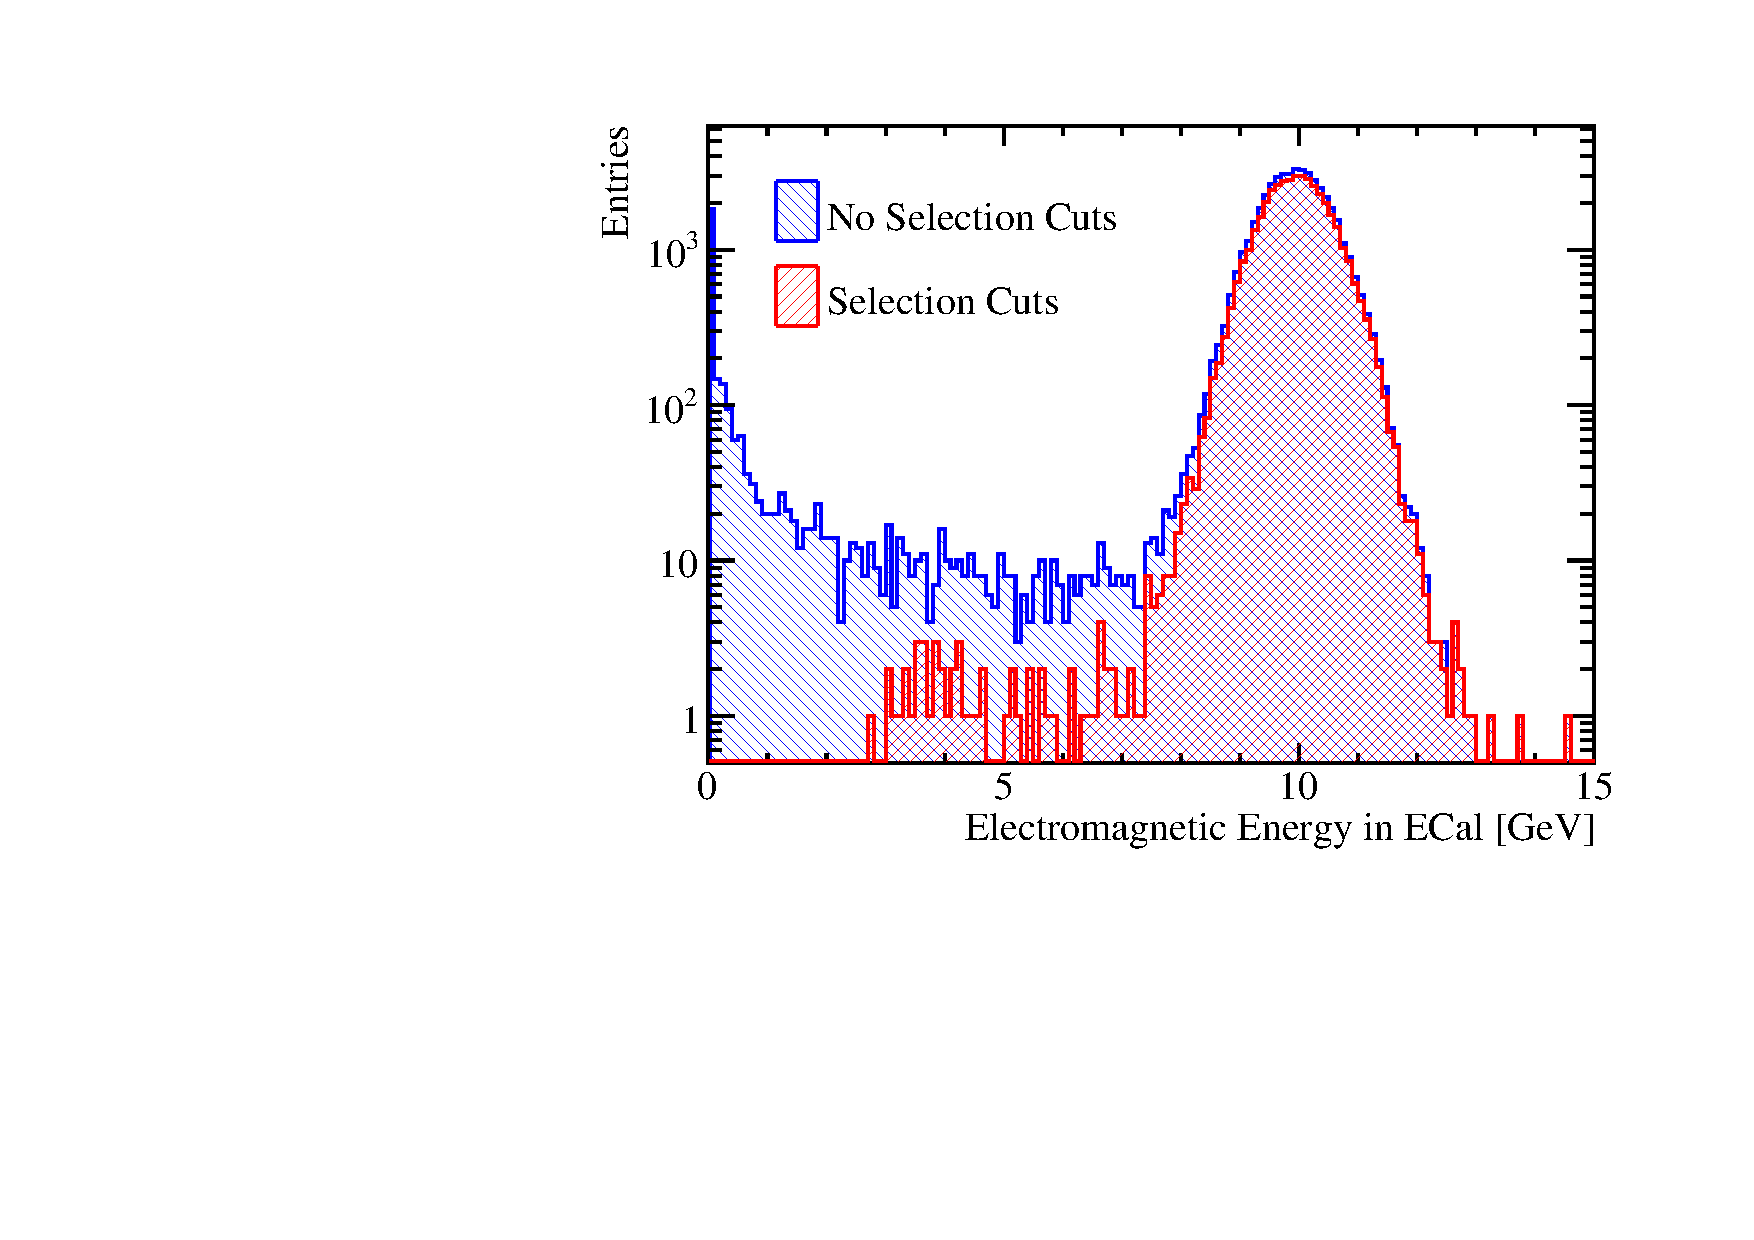
\includegraphics[width=0.5\textwidth]{EnergyEstimators/Plots/Calibration/EMScaleSetting/EMScaleECalSelection.pdf}
\caption[Sum of the electromagnetic energy measured in the ECal for 10 GeV $\gamma$ events with and without the selection cuts.]{Sum of the electromagnetic energy measured in the ECal for 10 GeV $\gamma$ events with and without the selection cuts.}
\label{fig:ecalemscaleselection}
\end{figure}

\begin{figure}
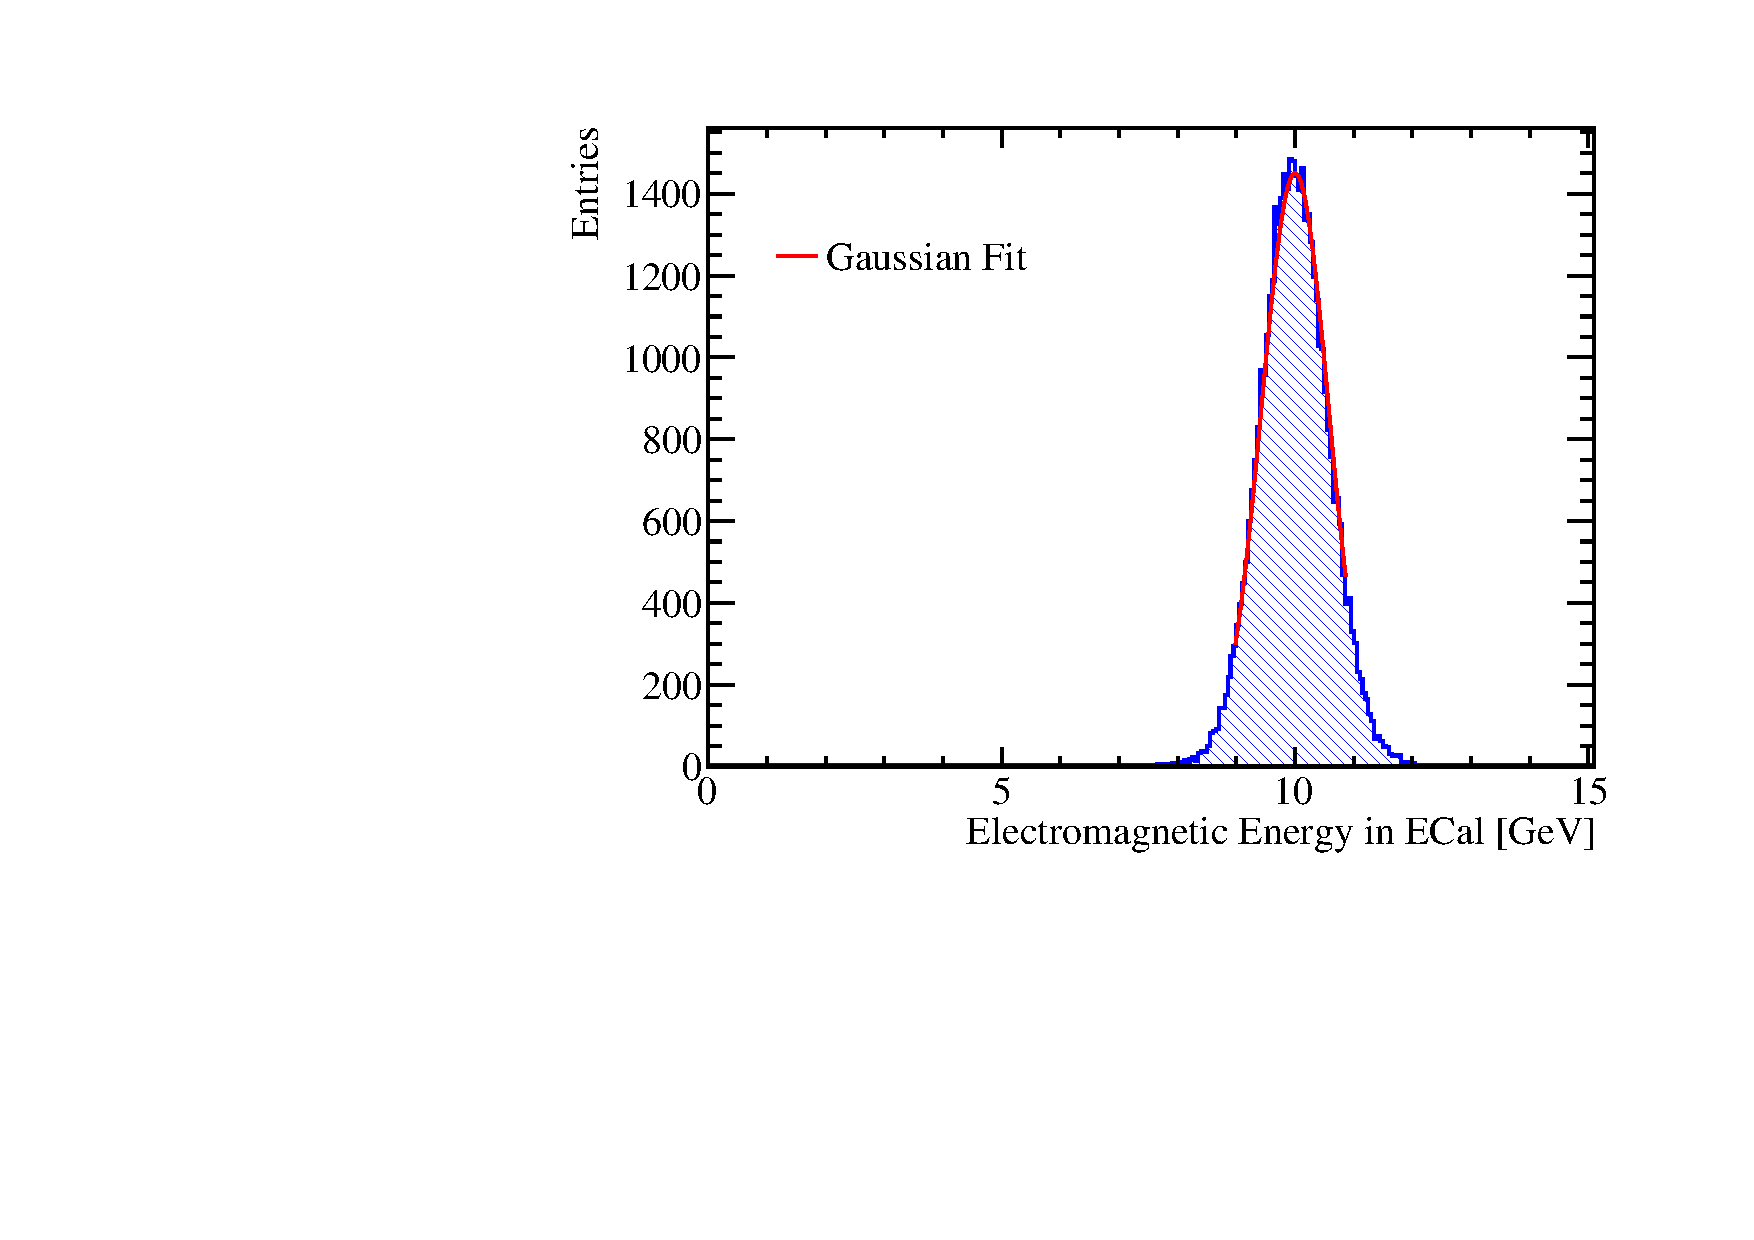
\includegraphics[width=0.5\textwidth]{EnergyEstimators/Plots/Calibration/EMScaleSetting/EMScaleSettingECalFit.pdf}
\caption[Gaussian fit to sum of the electromagnetic energy deposited in the ECal for 10 GeV $\gamma$ events with selection cuts.]{Gaussian fit to sum of the electromagnetic energy deposited in the ECal for 10 GeV $\gamma$ events with selection cuts.}
\label{fig:ecalemscalefit}
\end{figure}

The fitting procedure follows that used for the ECal digitisation, described in section \ref{sec:ecaldigi}, whereby a trial calibration for the electromagnetic energy scale in the ECal, $\beta^{EM0}_{ECal}$, is assumed and the single $\gamma$ events simulated.  The distribution of the electromagnetic energy in the ECal is created and a Gaussian fit applied to the range of data with the smallest root mean square containing at least 90 \% of the data.  The mean of this fit, $E_{\text{Fit}}$, is then used to scale $\beta^{EM0}_{ECal}$ in the following way

\begin{equation}
\beta^{EM0}_{ECal} \rightarrow \beta^{EM}_{ECal} = \beta^{EM0}_{ECal} \times \frac{E_{MC}}{E_{Fit}}
\end{equation}

An example distribution and fit used in the calibration of the nominal ILD detector model can be found in figure \ref{fig:ecalemscalefit}.  This procedure is repeated using the updated $\beta^{EM}_{ECal}$ until $E_{\text{Fit}}$ falls within a specified tolerance.  The tolerance applied here was $|E_{\text{Fit}} - E_{\text{MC}}| < E_{\text{MC}} \times 0.5 \%$.  The binning for the fitted histogram is chosen such that the bin width is equal to the desired target tolerance on $E_{\text{Fit}}$ e.g. $E_{\text{MC}} \times 0.5 \% = 0.05$ GeV.  This tolerance is tighter than was applied for the digitisation as it is these energies that are used in downstream analyses.   
 
The electromagnetic scale in the HCal, $\beta^{EM}_{HCal}$, is chosen to be equal to the hadronic scale in the HCal, $\beta^{Had}_{HCal}$.  The details of the determination of $\beta^{Had}_{HCal}$ can be found in section \ref{sec:hadscalesetting}.  For the ILC and CLIC, $\beta^{EM}_{HCal}$ is not a critical parameter in the reconstruction as photons are largely contained within the ECal meaning little to no electromagnetic energy is measured in the HCal.  

%========================================================================================

\subsubsection{Hadronic scale setting}
\label{sec:hadscalesetting}
The hadronic scale in the ECal, $\beta^{Had}_{ECal}$, is important to detector performance as a non-negligible amount of hadronic energy will be measured in the ECal.  As the ECal contains $\approx 1 \lambda_{I}$, the hadronic scale in the ECal cannot be independently set as it is unfeasible to create a large sample of 20 GeV $K^{0}_{L}$ events that are fully contained within it.  Therefore, the hadronic scale in the ECal and HCal have to be set simultaneously.  

Cuts are applied to select the $K^{0}_{L}$ events that are appropriate to use for the hadronic scale calibration.  The last layer in which energy is deposited in the HCal must not occur in the back 10 \% of the HCal.  This ensures that the event does not suffer from leakage of energy out of the back of the HCal.  A single neutral hadron must be reconstructed to veto events with reconstruction failures.  Finally, the total hadronic energy measured in ECal and HCal, $E^{Had}_{ECal} + E^{Had}_{HCal}$, must fall within 3 $\sigma$ of the desired hadronic energy distribution, $E^{Had}_{ECal} + E^{Had}_{HCal} = 20 \text {GeV} - m_{K^{0}_{L}} = E_{K}$.  $\sigma$ is defined to be $55\% \times \sqrt{E} = 2.46 \text{GeV}$ for 20 GeV $K^{0}_{L}$.  This definition for sigma is used as it matches the energy resolution as a function of energy for neutral hadrons using the nominal ILD HCal \cite{Behnke:2013lya}.  This cut ensures that when fitting the two dimensional distribution of hadronic energy measured in the ECal and HCal outliers do not skew the fit.  Once again the target reconstructed energy for this sample is the kinetic energy and not the total energy of the $K^{0}_{L}$ for the reasons outlined in section \ref{sec:hcaldigi}.  The impact of cuts are illustrated in figure \ref{fig:hadscaleselection}.

\begin{figure}
\subfloat[]{\label{fig:hadscaleselectionnocuts}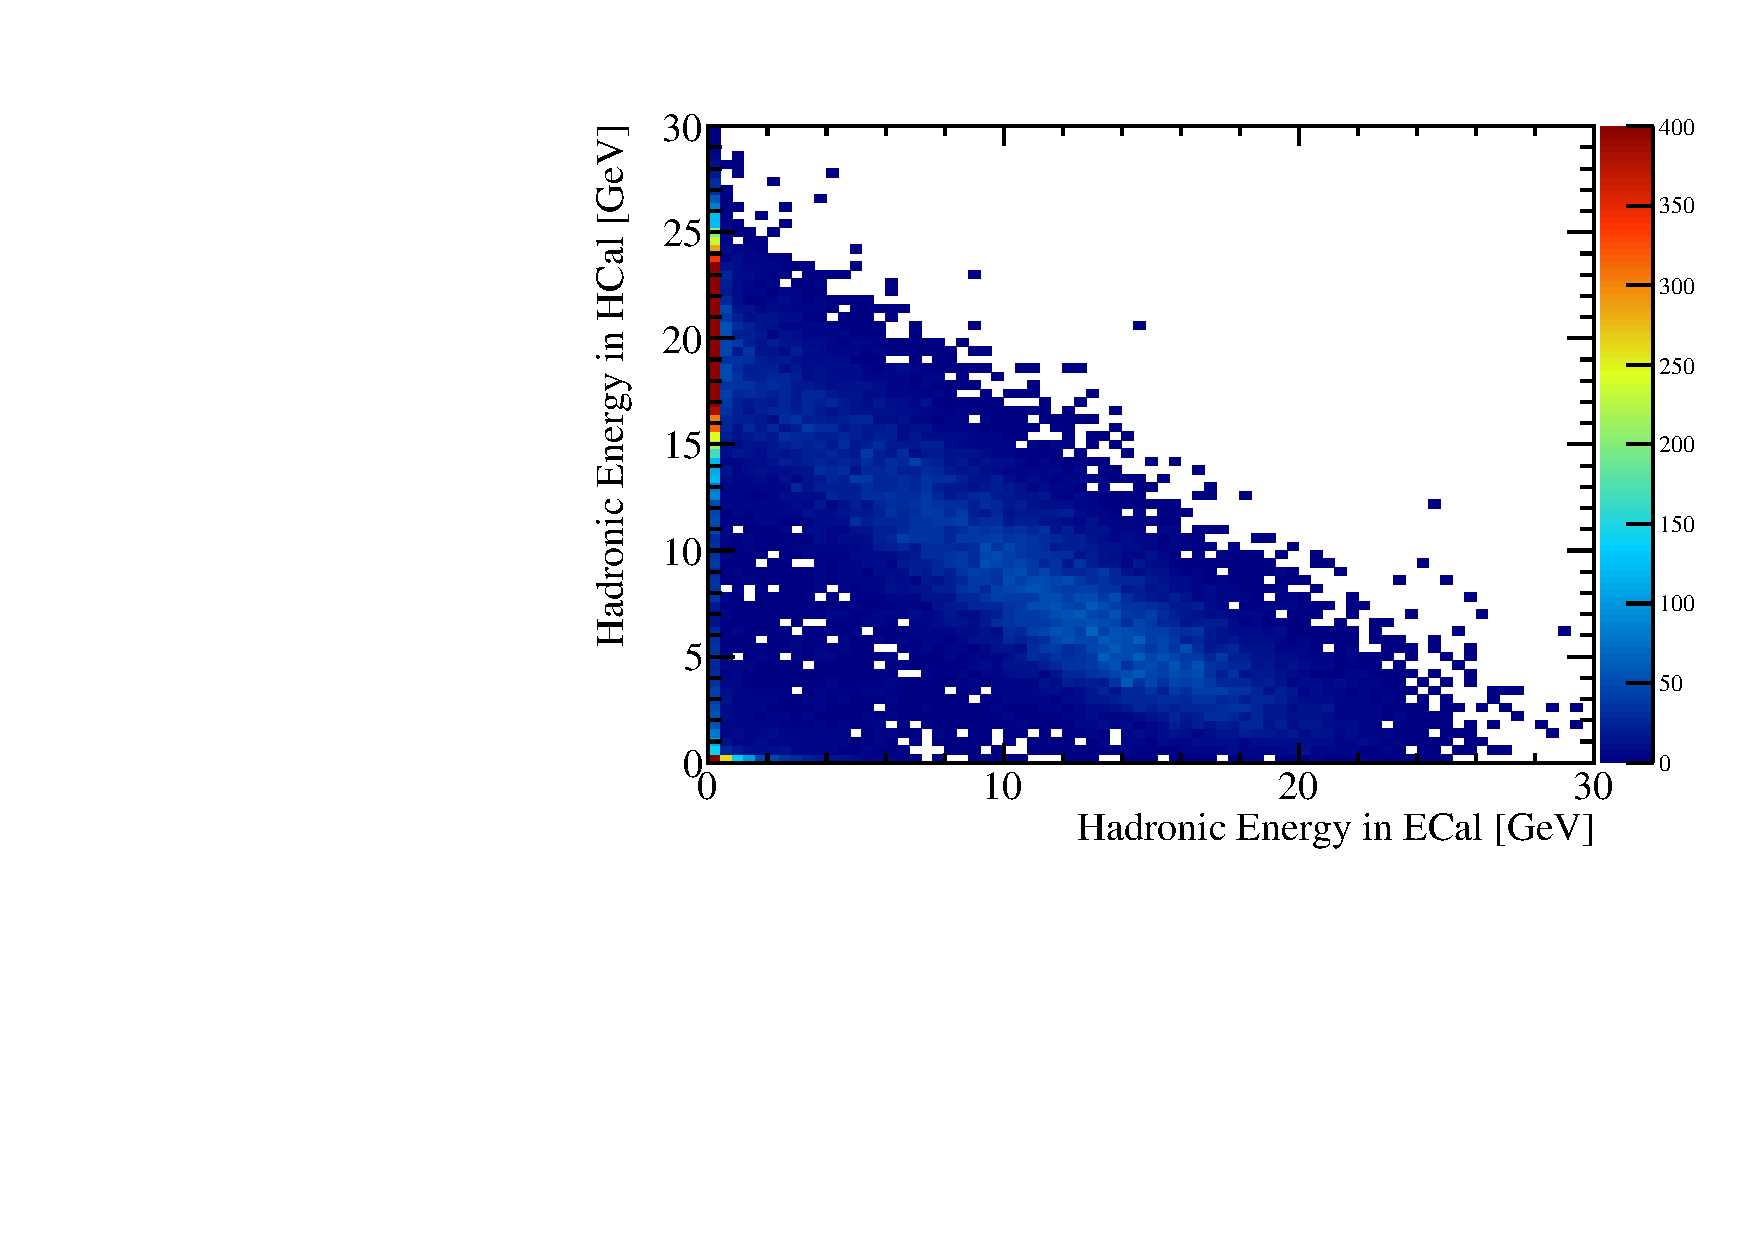
\includegraphics[width=0.5\textwidth]{EnergyEstimators/Plots/Calibration/HadScaleSetting/HadScaleECalHCalSelectionNoCuts.pdf}}
\subfloat[]{\label{fig:hadscaleselectioncuts}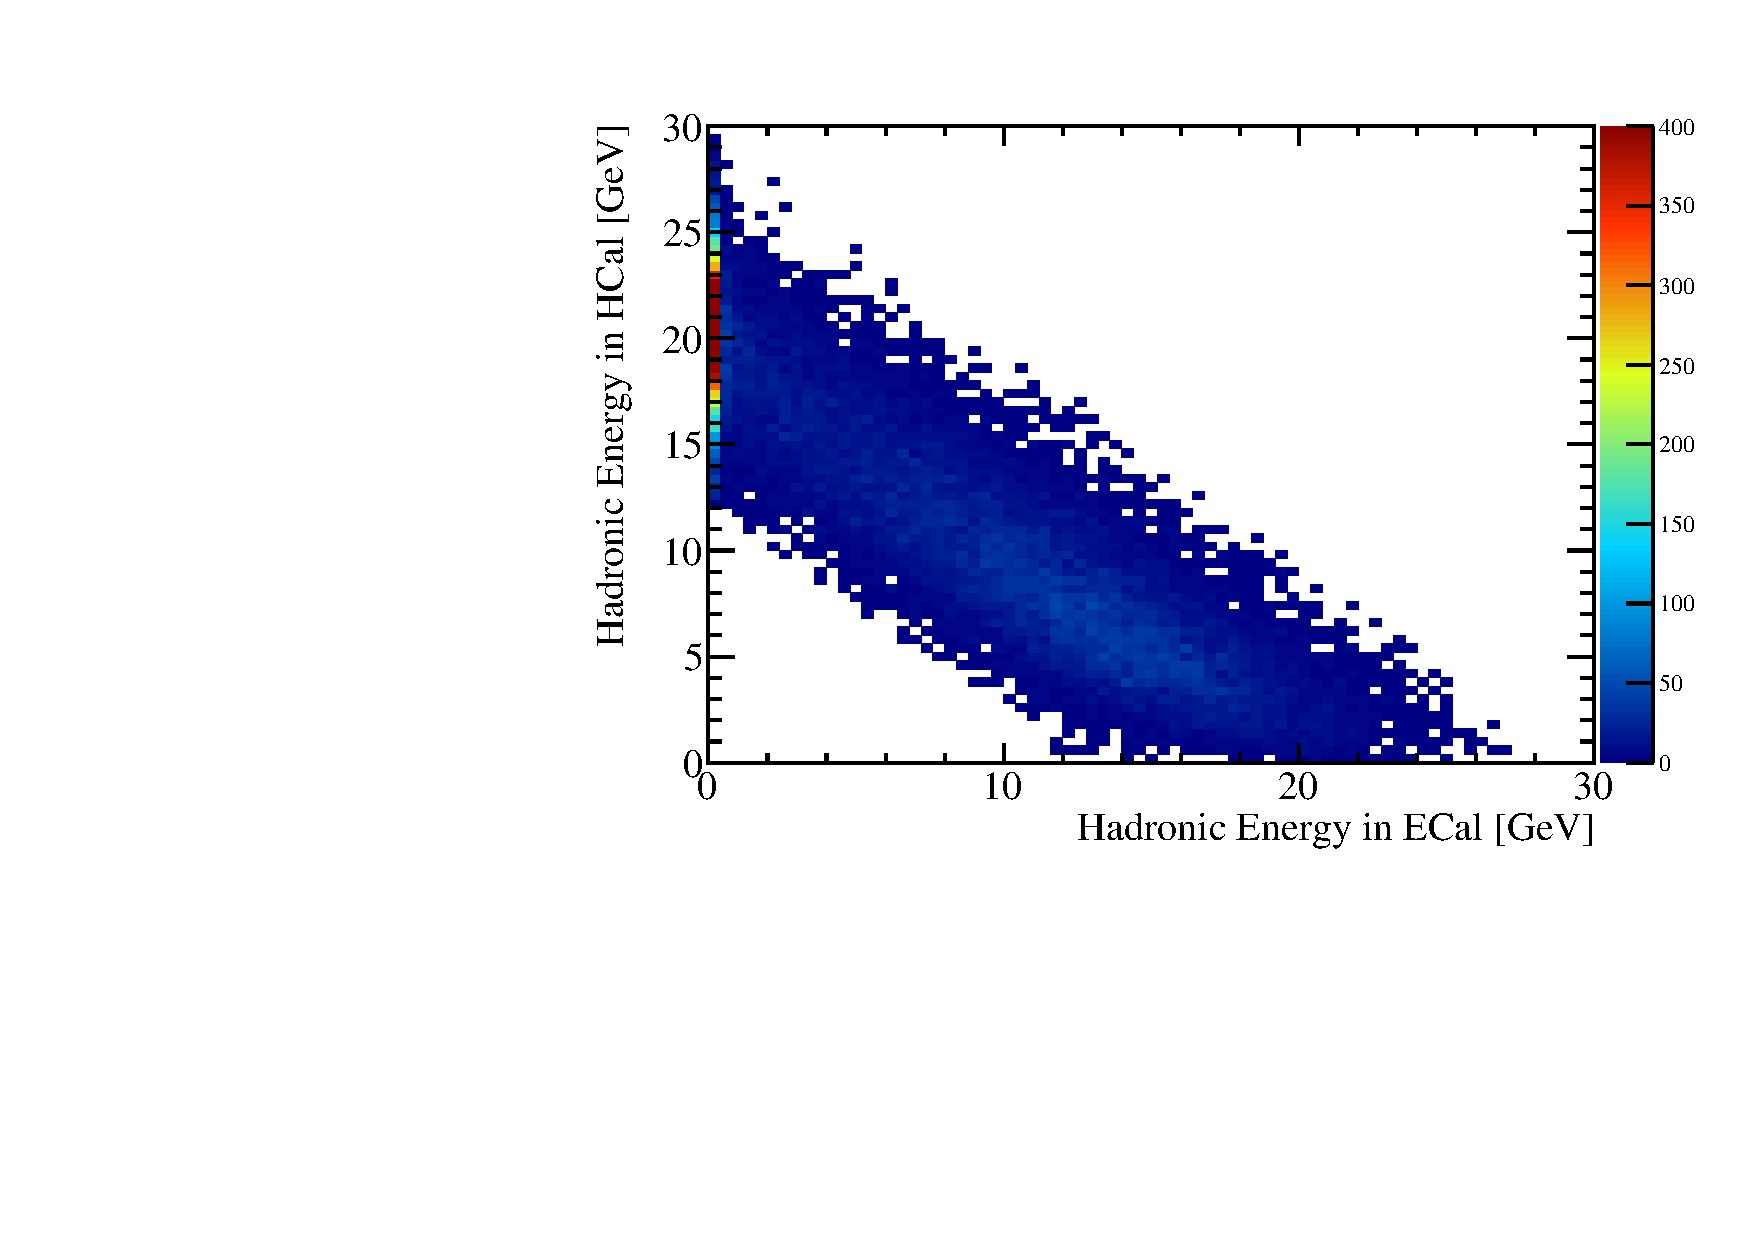
\includegraphics[width=0.5\textwidth]{EnergyEstimators/Plots/Calibration/HadScaleSetting/HadScaleECalHCalSelectionCuts.pdf}}
\caption[The distribution of hadronic energy measured in the ECal and HCal for 20 GeV $K^{0}_{L}$ events with and without selection cuts.]{The distribution of hadronic energy measured in the ECal and HCal for 20 GeV $K^{0}_{L}$ events \protect\subref{fig:hadscaleselectionnocuts} without selection cuts and \protect\subref{fig:hadscaleselectioncuts} with selection cuts.}
\label{fig:hadscaleselection}
\end{figure}

This part of the calibration procedure is again iterative and begins by assuming trial values, $\beta^{Had0}_{ECal}$ and $\beta^{Had0}_{ECal}$, for the hadronic scale calibration factors $\beta^{Had}_{ECal}$ and $\beta^{Had}_{ECal}$.  The 20 GeV $K^{0}_{L}$ events are then simulated and reconstructed.  Following that a linear fit to the distribution of $E^{Had}_{ECal}$ against $E^{Had}_{HCal}$ for 20 GeV $K^{0}_{L}$ events passing the selection cuts is applied.  The fit is performed by minimising $\chi^{2}$, which is defined as

\begin{equation}
\chi^{2}(\delta^{Had}_{ECal}, \delta^{Had}_{HCal}) = \sum_{i} \frac{x_{i}}{\sigma_{x_{i}}}
\end{equation}

where $x_{i}$ is the perpendicular distance from $E^{Had}_{ECal}$ and $E^{Had}_{HCal}$ for event $i$ to the line $E^{Had}_{HCal} = \delta^{Had}_{HCal} - E^{Had}_{ECal} \frac{\delta^{Had}_{HCal}}{\delta^{Had}_{ECal}}$.   The definition of $x_{i}$ is given in equation \ref{equ:xicalc}, but best illustrated by considering figure \ref{fig:hadscalechi2calc}.  $\sigma_{x_{i}}$ is the uncertainty on $x_{i}$, which is calculated by propagating the uncertainties on $E^{Had}_{ECal}$ and $E^{Had}_{HCal}$, which are assumed to be $\sigma_{E^{Had}_{E/HCal}} = 55\% \times \sqrt{E^{Had}_{E/HCal}}$, into the expression for $x_{i}$.  The result of this propagation of errors is given in equation \ref{equ:sigmaxicalc}.  The sum runs over all events, $i$, passing the selection cuts.  

\begin{figure}
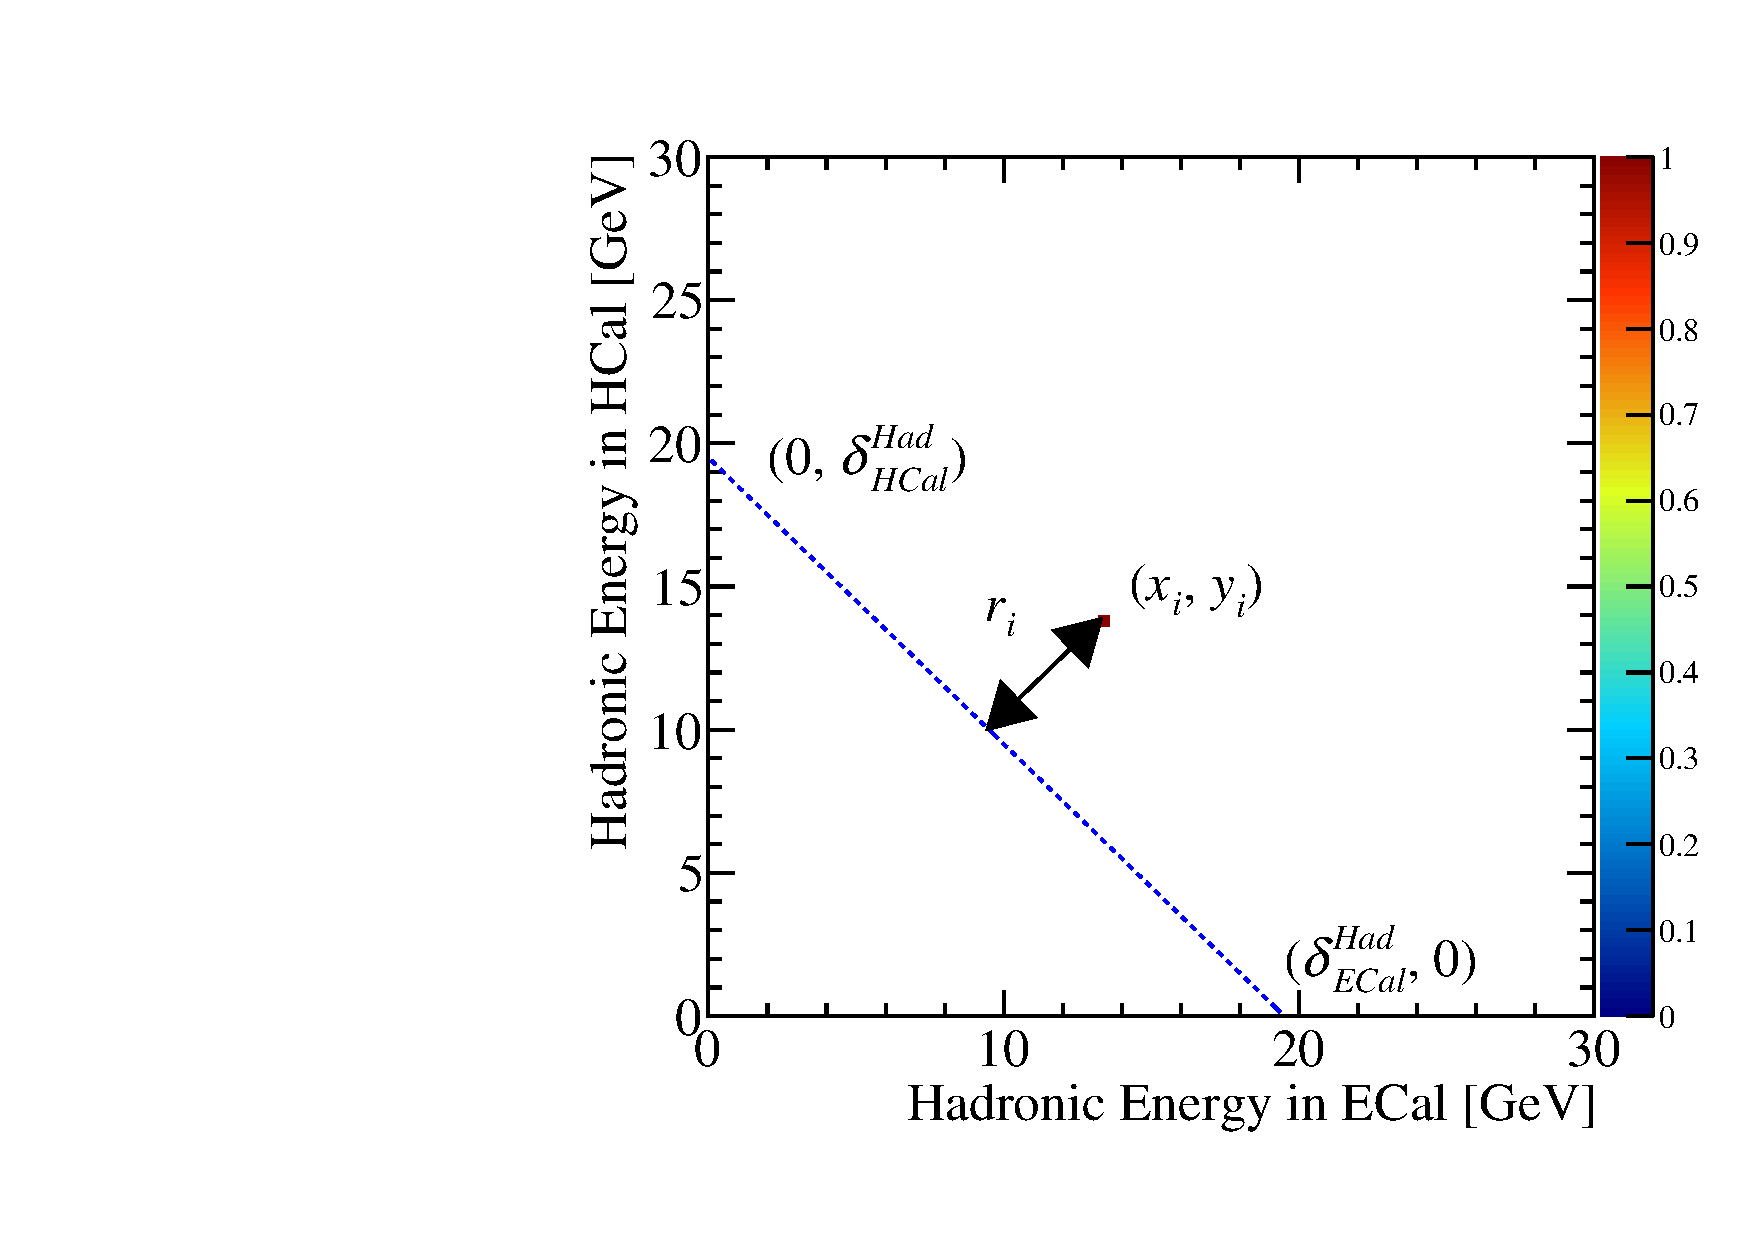
\includegraphics[width=0.5\textwidth]{EnergyEstimators/Plots/Calibration/HadScaleSetting/HadScaleECalHCalSelectionExample.pdf}
\caption[An example showing the definition of $x_{i}$, the variable used for the calculation of $\chi^{2}(\delta^{Had}_{ECal}, \delta^{Had}_{HCal})$ for the setting of the hadronic energy scale.]{An example showing the definition of $x_{i}$, the variable used for the calculation of $\chi^{2}$ for the setting of the hadronic energy scale.  For an event that has been measured with hadronic energy $E^{Had}_{ECal}$ in the ECal and $E^{Had}_{HCal}$ in the HCal, the geometric interpretation of $x_{i}$ is shown.  The blue dotted line is defined as $E^{Had}_{HCal} = \delta^{Had}_{HCal} - E^{Had}_{ECal} \frac{\delta^{Had}_{HCal}}{\delta^{Had}_{ECal}}$.}
\label{fig:hadscalechi2calc}
\end{figure}

\begin{equation}
x_{i} = \frac{E^{Had}_{HCal} \delta^{Had}_{ECal} + E^{Had}_{ECal} \delta^{Had}_{HCal} - \delta^{Had}_{ECal} \delta^{Had}_{HCal}}{\sqrt{(\delta^{Had}_{ECal})^{2} + (\delta^{Had}_{HCal})^{2}}}
\label{equ:xicalc}
\end{equation}

\begin{equation}
\sigma_{i} = \frac{(\sigma_{E^{Had}_{HCal}}  \delta^{Had}_{ECal})^{2} + (\sigma_{E^{Had}_{ECal}} \delta^{Had}_{HCal})^{2}}{\sqrt{(\delta^{Had}_{ECal})^{2} + (\delta^{Had}_{HCal})^{2}}}
\label{equ:sigmaxicalc}
\end{equation}

The minimisation is done by stepping a range of $\delta^{Had}_{ECal}$ and $\delta^{Had}_{HCal}$ centred about the ideal value of $20 \text { GeV} - m_{K^{0}_{L}}$ in search for the minimum $\chi^{2}$.  Once the minima in $\chi^{2}$ is found the trial calibration factors $\beta^{Had0}_{ECal}$ and $\beta^{Had0}_{ECal}$ are rescaled to correct for any deviation from the desired fit as follows

\begin{equation}
\beta^{Had0}_{ECal} \rightarrow \beta^{Had}_{ECal} = \beta^{Had0}_{ECal} \times \frac{E_{K}}{\Delta^{Had}_{ECal}} \\
\beta^{Had0}_{HCal} \rightarrow \beta^{Had}_{HCal} = \beta^{Had0}_{HCal} \times \frac{E_{K}}{\Delta^{Had}_{HCal}}
\end{equation}

where $\Delta^{Had}_{ECal}$ and $\Delta^{Had}_{ECal}$ are the values of $\delta^{Had}_{ECal}$ and $\delta^{Had}_{ECal}$ giving the minimum $\chi^{2}$.  The step sizes used for minimising $\chi^{2}$ with respect to $\delta^{Had}_{ECal}$ and $\delta^{Had}_{ECal}$ is chosen such that a single step corresponds to the target final tolerance on $\delta^{Had}$ i.e. $|\delta^{Had}_{E/HCal} - E_{\text{MC}}| < E_{\text{MC}} \times 0.5 \% \approx 0.1 \text{GeV}$.  

This procedure is then repeated until $\Delta^{Had}_{ECal}$ and $\Delta^{Had}_{ECal}$ both fall within a given tolerance, which in this case it taken to be $|\Delta^{Had}_{E/HCal} - E_{\text{MC}}| < E_{\text{MC}} \times 0.5 \% \approx 0.1 \text{GeV}$

%========================================================================================

\subsection{Calibration step ordering}
\label{sec:orderingcalib}

The calibration procedure has to be run in the following order so that the building blocks used for each stage of the calibration procedure can be assumed to be correctly calibrated:

\begin{enumerate}
\item MIP Scale setting in the digitiser as described in section \ref{sec:mipresponse}.
\item Calibration of digitisation of calorimeter hits in the ECal and HCal as described in section \ref{sec:digi}.
\item MIP Scale setting in PandoraPFA as described in section \ref{sec:mipresponse}.
\item Electromagnetic and hadronic scale settings in PandoraPFA as described in section \ref{sec:scalesetting}.
\end{enumerate}

%========================================================================================

\subsection{Retraining photon likelihood data}
PandoraPFA uses likelihood data in the identification of $\gamma$s.  Data related to the topology and energy of electromagnetic showers and the wider event environment is used to determine whether a given shower is likely to be a $\gamma$.  The likelihood data is trained using off-shell mass Z boson (Z') events at 500 GeV that decay into light quarks (u, d, s).  It is necessary to retrain this data only when varying the ECal as photons are contained largely within the ECal at the energies being considered and the likelihood data only uses measurements made in the ECal.

As this data uses post digitisation hits it is important to ensure that a fully calibrated detector is used when retraining the likelihood data.  Therefore, it is necessary to run the calibration procedure, as described in section \ref{sec:orderingcalib}, before retaining.  However, as the reconstruction uses likelihood data the calibration procedure must be performed twice.  Initially the calibration procedure is performed where PandoraPFA is run without the inclusion of this likelihood data, using PandoraSettingsMuon.xml.  Then the likelihood data is retrained using the results of the first calibration pass and then the retrained likelihood data is used in the second pass of the calibration procedure.  

In the optimisation studies presented in chapter OPTIMISATION STUDIES this procedure was followed whenever the ECal was modified so that optimal detector performance was achieved.  

%========================================================================================
%========================================================================================

\section{HCal Cell Truncation}
\label{sec:hcalcelltruncation}
A powerful tool used by PandoraPFA in event reconstruction is the application of a truncation to the maximum amount of energy that can be recorded in a calorimeter cell in the HCal.  The purpose of this truncation is to eliminate the effect of spuriously high energy calorimeter cells that would skew the reconstruction.  The origin of these high energy cells is twofold: showering particles may be moving within the plane of the active material, which can lead to an overestimation of the deposited energy if the shower is not sufficiently uniform across the full cell, and Landau fluctuations \cite{Landau:1944if}, which originate from high energy knock-on electrons appearing within particle showers \cite{Bichsel:2004ej}.  These effects are only relevant in hadronic showers as electromagnetic showers begin showering almost immediately within the ECal, meaning they are unlikely to be directed within the plane of the active material of the calorimeter, and the Landau distribution only describes the energy loss for charged particles.  This means showering $\gamma$ do not produce Landau fluctuations and neither do $e^{-}$ and $e^{+}$ as their energy, in the particle flow paradigm, arises from the curvature of the track they produce and not the calorimeter hits.  Therefor, as only hadronic showers produce spuriously high energy cells through these mechanisms, this truncation is only applied on HCal cells.  

A great deal of care has to be given to the truncation energy so that cells from typical hadronic shower development are not truncated, while the spuriously high energy cells are.  This can be illustrated by considering the single particle energy resolutions as a function of the HCal cell truncation that are shown in figure \ref{fig:ercelltrunc}.  The photon energy resolution is invariant to changes in the cell truncation as no photon energy is recorded in the HCal, while the energy resolution for the neutral hadrons is optimal for a truncation of 1 GeV.  This indicates that a  GeV truncation is sufficient for dealing with the Landau fluctuations and showering particles travelling within the active material of the calorimeter cell.  For cell truncations greater than 1 GeV the resolution degrades as the spuriously high energy cells are not accounted for, while truncations below 1 GeV truncate energy measurements from typical hadronic shower development.  If typical hadronic shower cells are truncated this leads to a poorer sampling of the shower and a degradation in the energy resolution.  

\begin{figure}
\subfloat[]{\label{fig:ercelltruncphotons}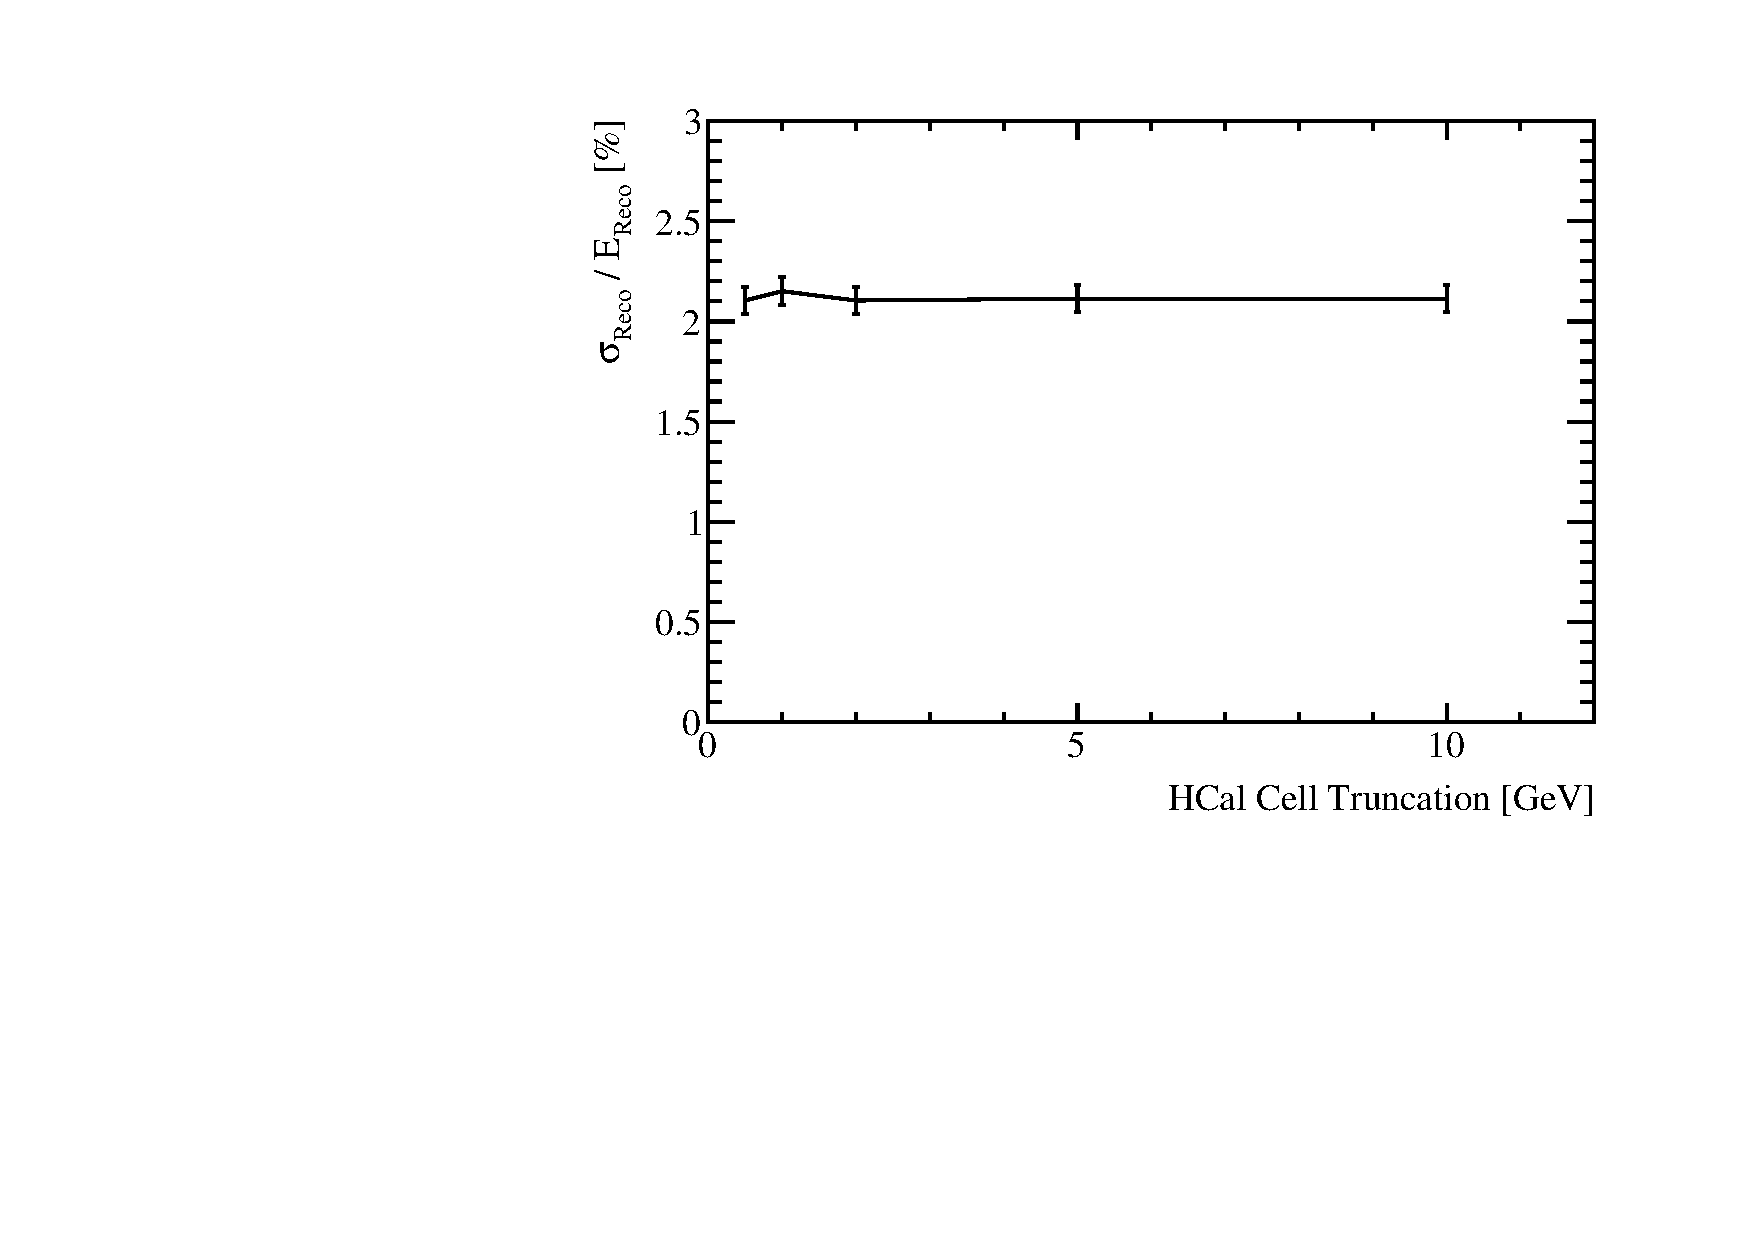
\includegraphics[width=0.5\textwidth]{EnergyEstimators/Plots/CellTruncation/ER_vs_PhotonCellTrunc_100GeVPhoton.pdf}}
\subfloat[]{\label{fig:ercelltrunckaons}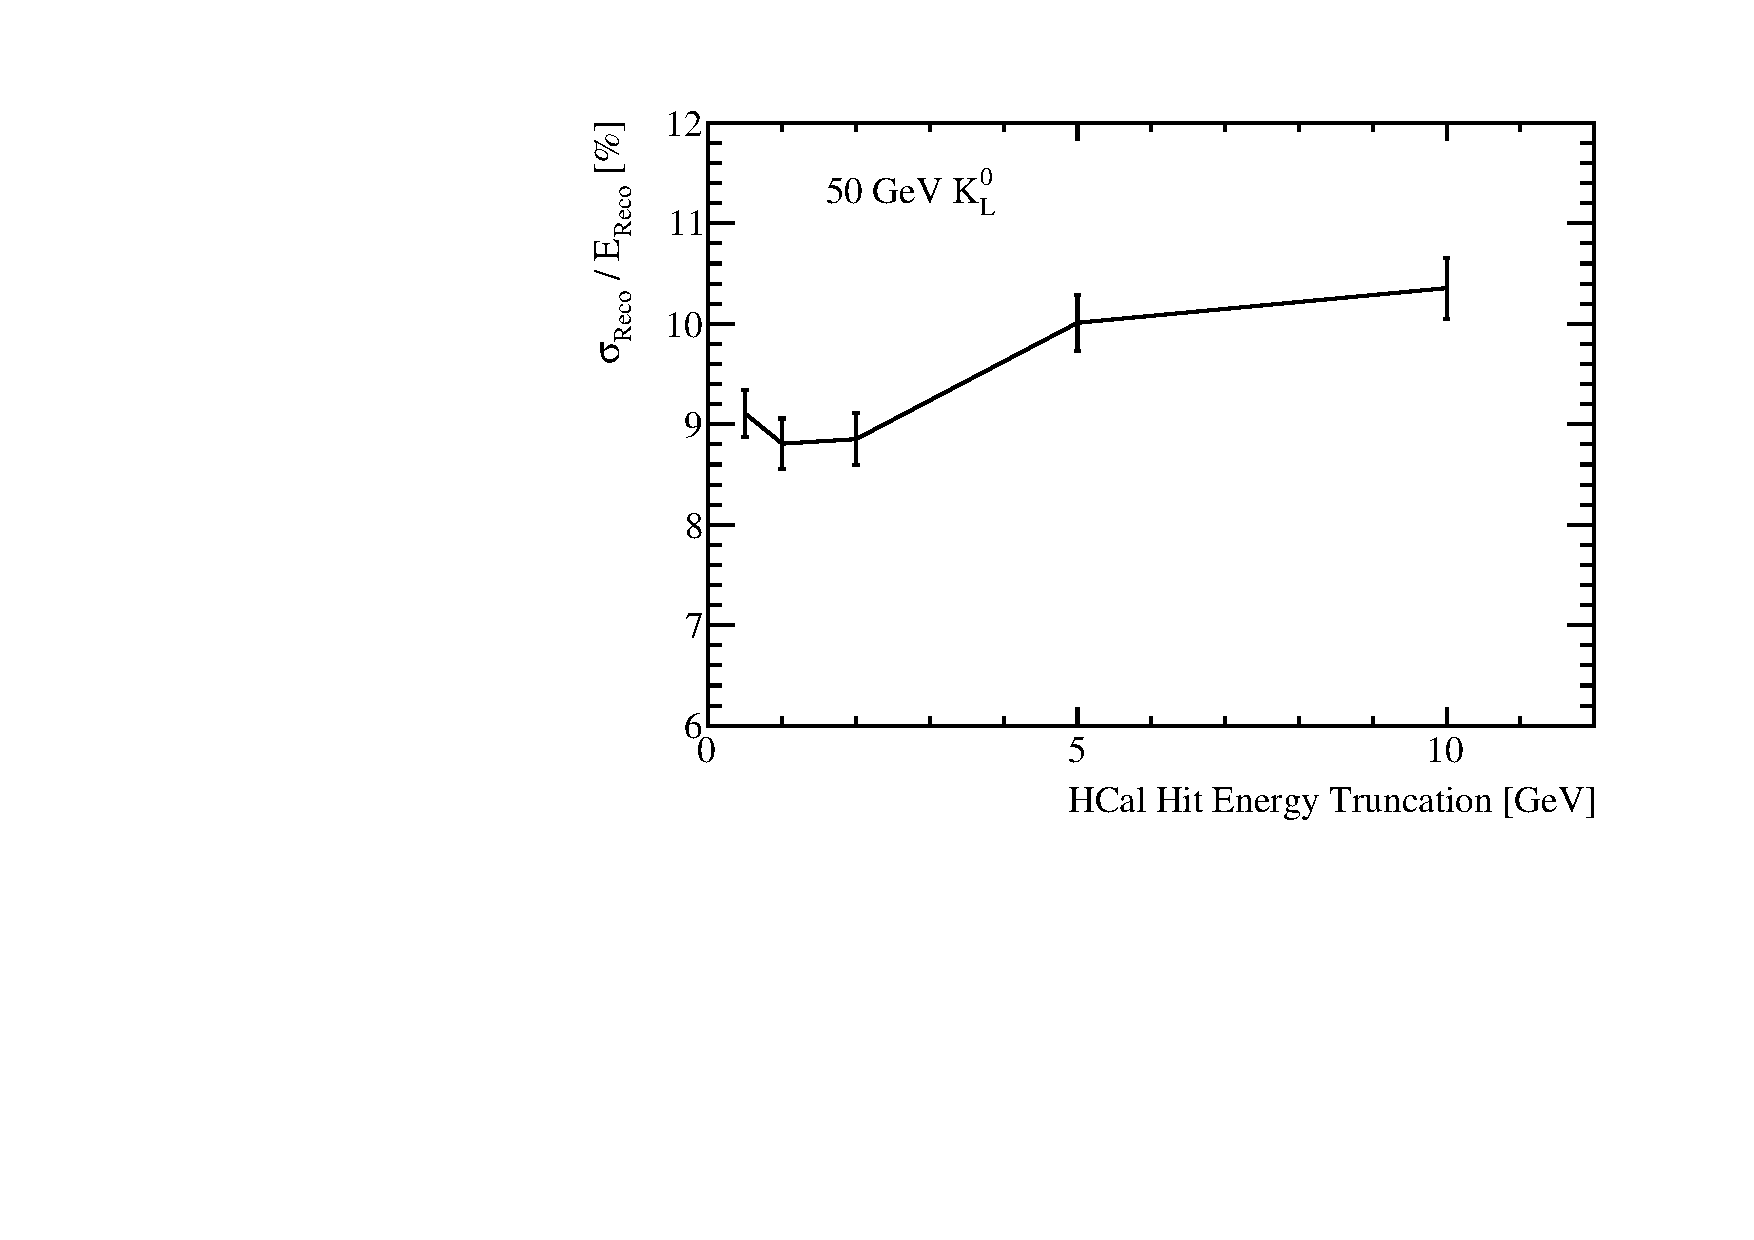
\includegraphics[width=0.5\textwidth]{EnergyEstimators/Plots/CellTruncation/ER_vs_Kaon0LCellTrunc_50GeVKaon0L.pdf}}
\caption[The energy resolution as a function of HCal cell truncation for \protect\subref{fig:ercelltruncphotons} 100 GeV $\gamma$ events and \protect\subref{fig:ercelltrunckaons} 50 GeV $K^{0}_{L}$ events for the nominal ILD detector model.]{The energy resolution as a function of HCal cell truncation for \protect\subref{fig:ercelltruncphotons} 100 GeV $\gamma$ events and \protect\subref{fig:ercelltrunckaons} 50 GeV $K^{0}_{L}$ events for the nominal ILD detector model.}
\label{fig:ercelltrunc}
\end{figure}

Once again, this effect propagates into the jet energy resolutions as shown by figure \ref{fig:jercelltrunc}.  The trends in this plot are complex as the optimal cell truncation varies with the jet energy.  At low energies a 0.5 GeV truncation gives the best performance, however, when the jet energies reach $\approx$ 180 GeV a 1-2 GeV truncation giving the best performance.  This is to be expected based on the Landau fluctuations.  The Landau distribution is essentially a Gaussian with a high energy tail and as the jet energy increases the definition of cell energies falling in the high energy tail changes.  Therefore, the definition of the cells requiring truncating changes as a function of jet energy and a procedure with more degrees of freedom than a single truncation value is required to fully account for this.  As particle showers grow in size with increasing incident particle energy it is expected that the problem of particles travelling within the active material plane, and not uniformly across the rest of the cell, should not change significantly with changes to the jet energy.  

When examining the breakdown of the jet energy resolutions into the intrinsic energy resolution and the confusion it was noted that the cell truncation improves both the intrinsic energy resolution and the confusion contribution to the jet energy resolution.  This indicates that the pattern recognition performed by PandoraPFA benefits from the absence of these spuriously high energy cells, which if not omitted can skew energy comparisons made in the reconstruction.  Any skewed energy comparisons in the reconstruction leads to inaccurate association of calorimeter hits to charged particle tracks.  In turn this causes double counting and/or omission of energy deposits in the calorimeters leading to a degradation of the energy resolution.  

\begin{figure}
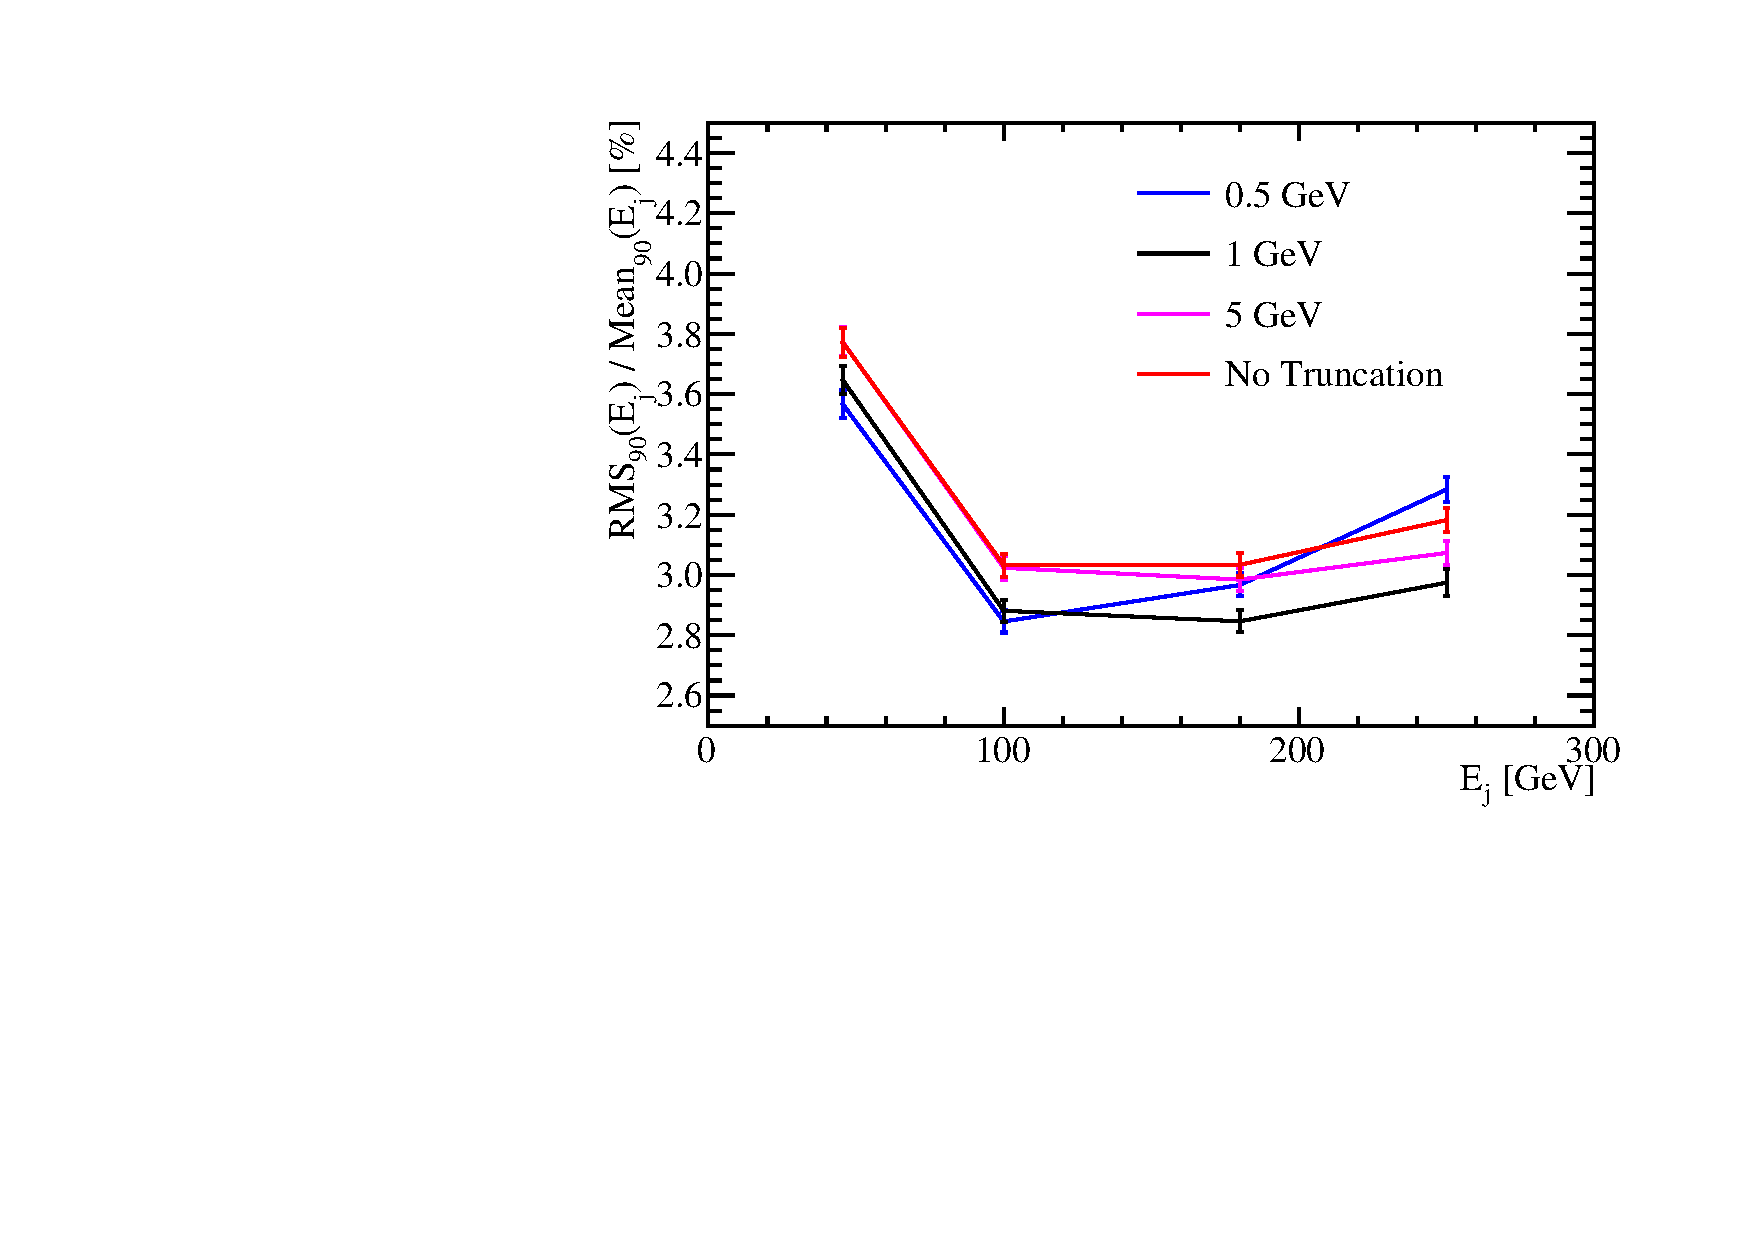
\includegraphics[width=0.5\textwidth]{EnergyEstimators/Plots/CellTruncation/JER_vs_JetEnergy_HCalCellTruncation.pdf}
\caption[The jet energy resolution as a function of jet energy for various hadronic cell truncations.  The results shown use the nominal ILD detector model.]{The jet energy resolution as a function of jet energy for various hadronic cell truncations.  The results shown use the nominal ILD detector model.}
\label{fig:jercelltrunc}
\end{figure}

While it is challenging to determine the optimal performance for a given detector model it is clear that applying an appropriate truncation produces significant improvement in detector performance.  Therefore, for the optimisation studies presented in section OPT STUDIES, the performance of each detector model is determined using a range of HCal cell truncations and the optimal resolutions quoted.  The HCal cell truncations considered in the optimisation were 0.5, 0.75, 1, 1.5, 2, 5, 10, and $10^{6}$ GeV (semi-infinite).  For the HCal cell size study the optimal performance for the 10, 20, 30, 40, 50 and 100 mm HCal cell size detector models was achieved using a 0.5, 0.75, 1, 1.5, 2 and 5 GeV truncation, for the tungsten HCal options the optimal truncation was 5 GeV and for all other detector models considered the optimal truncation was 1 GeV.  This optimisation has a significant impact on detector optimisation, which can be seen by comparing the jet energy resolutions using the optimised cell truncation and a uniform 1 GeV truncation, as found in \ref{fig:jerhcalcellopt}.  Without this optimisation of cell truncation the significance of the HCal cell size is overinflated and could have led to a misinformed detector design choice.  

\begin{figure}
\subfloat[]{\label{fig:jerhcalcelloptgoodtrunc}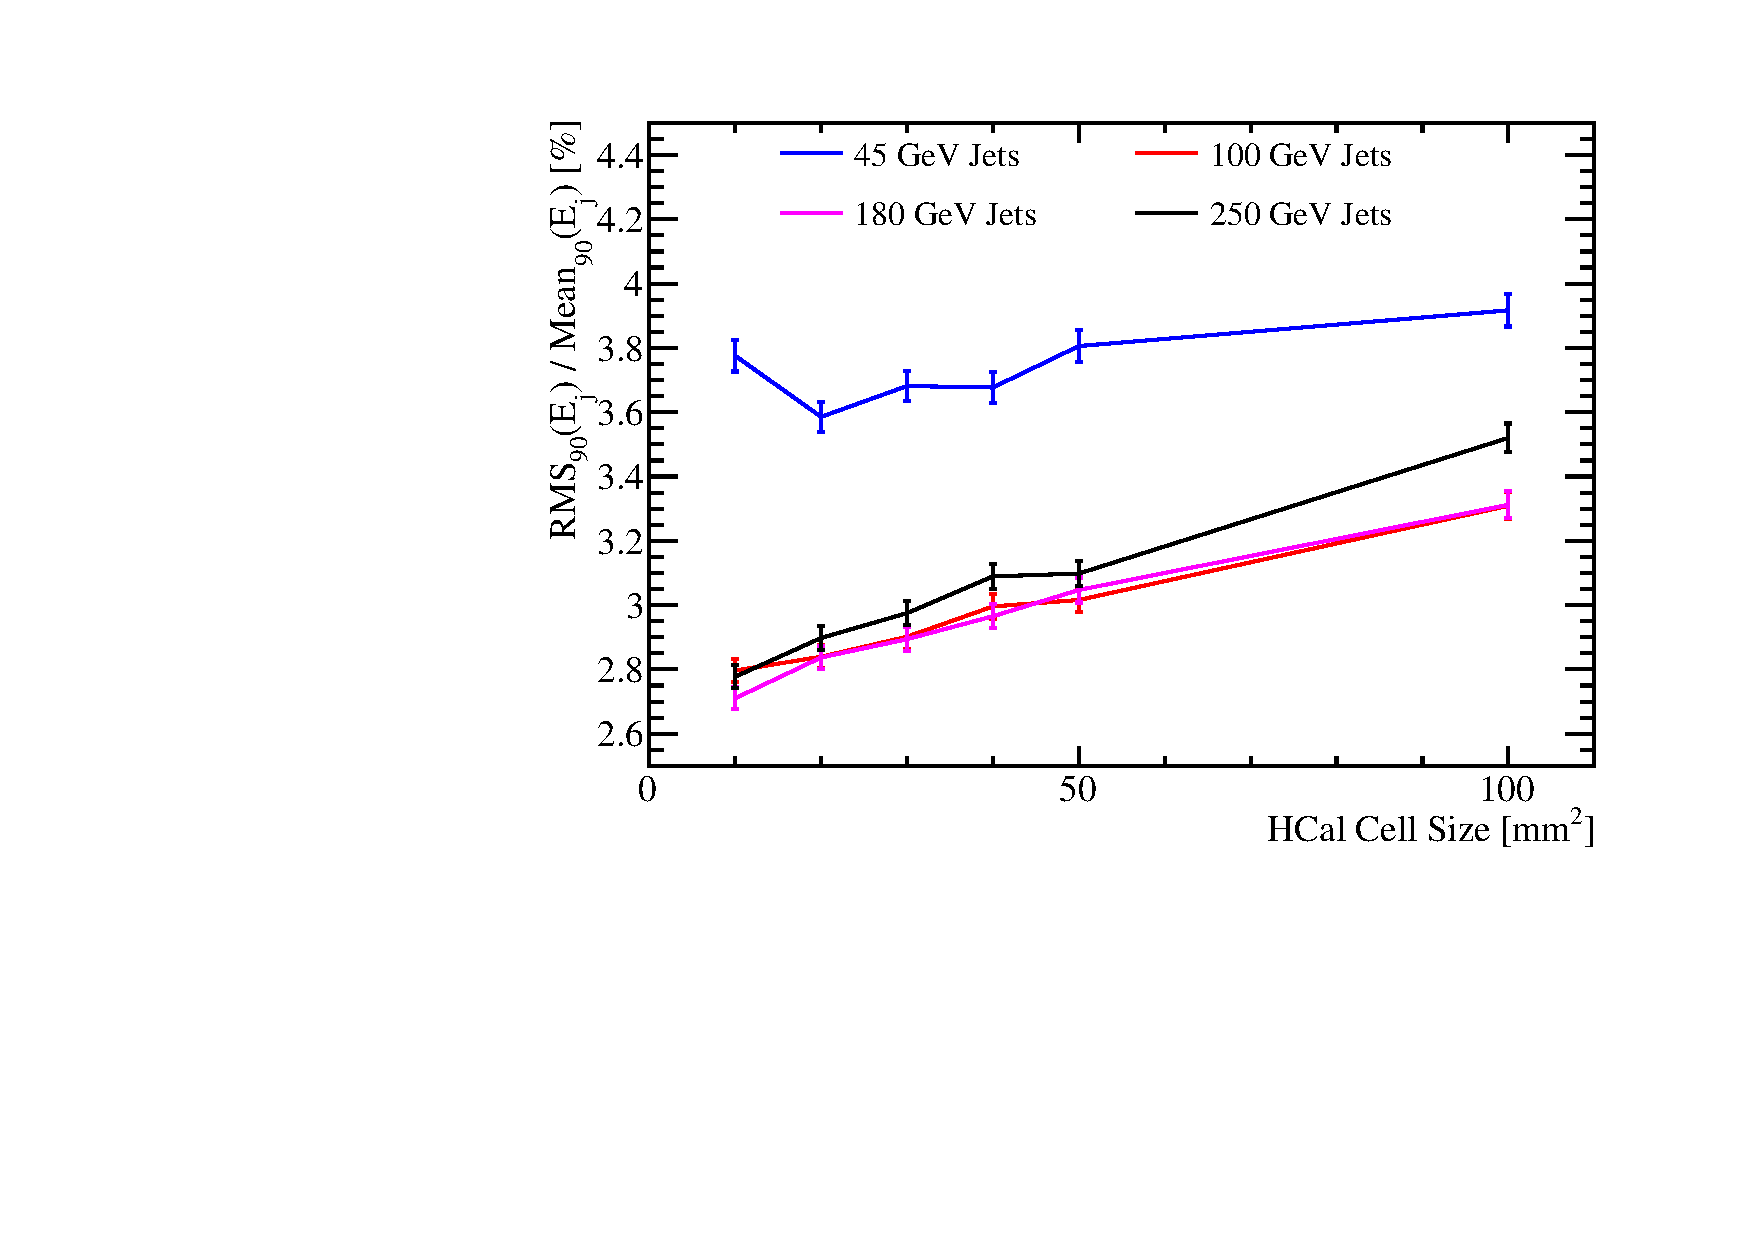
\includegraphics[width=0.5\textwidth]{OptimisationStudies/Plots/JetEnergyResolutions/JER_vs_HCalCellSize.pdf}}
\subfloat[]{\label{fig:jerhcalcelloptbadtrunc}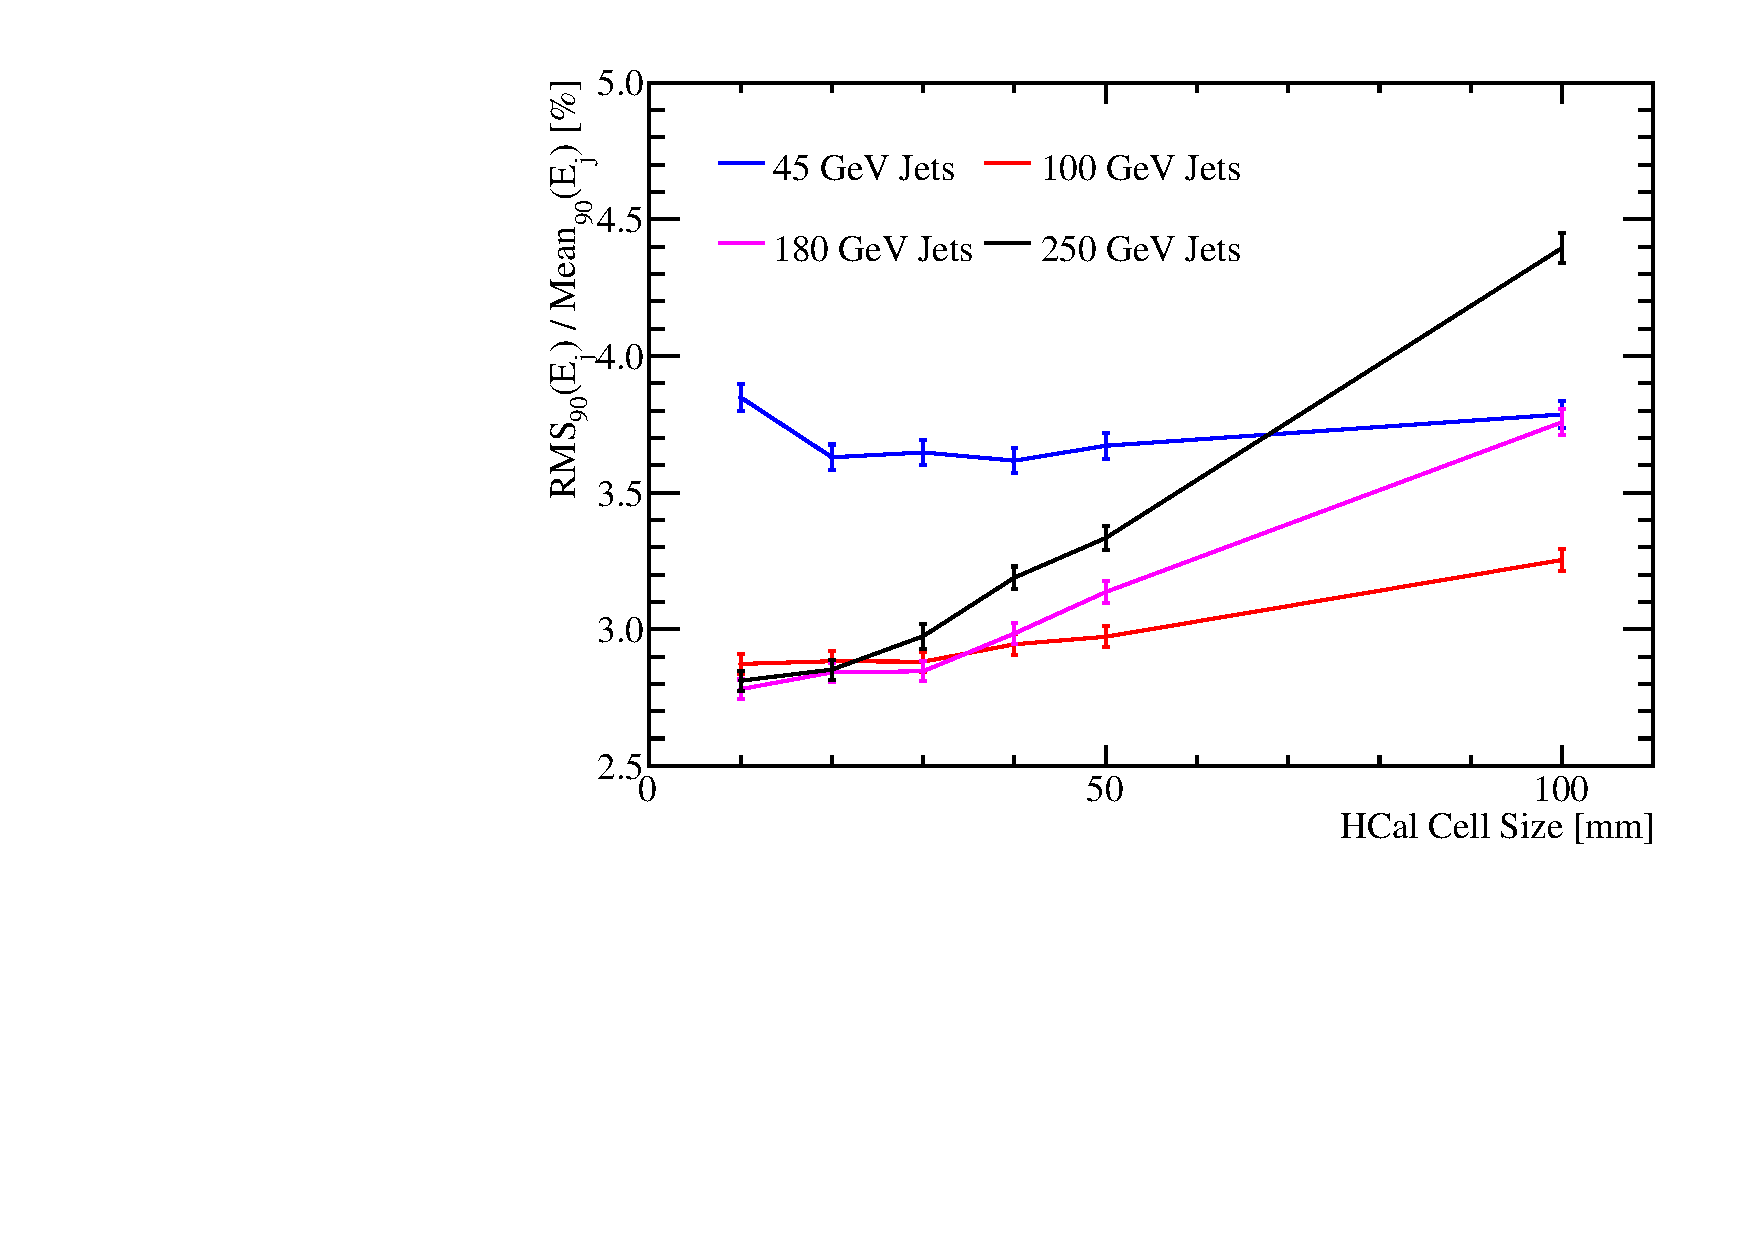
\includegraphics[width=0.5\textwidth]{EnergyEstimators/Plots/CellTruncation/JER_vs_HCalCellSizeBadTruncation.pdf}}
\caption[The jet energy resolution as a function of HCal cell size using \protect\subref{fig:jerhcalcelloptgoodtrunc} an optimised HCal cell truncation and \protect\subref{fig:jerhcalcelloptbadtrunc} a fixed 1 GeV truncation.]{The jet energy resolution as a function of HCal cell size using \protect\subref{fig:jerhcalcelloptgoodtrunc} an optimised HCal cell truncation and \protect\subref{fig:jerhcalcelloptbadtrunc} a 1 GeV truncation.}
\label{fig:jerhcalcellopt}
\end{figure}

%========================================================================================
%========================================================================================

\section{Software Compensation}
\label{sec:softcomp}
As discussed in chapter CALORIMETERS CHAPTER, the response of a calorimeter to a hadronic shower is different to that of an electromagnetic showers.  The particle shower produced by a hadron when passing through a calorimeter has two components,\cite{Wigmans:2000vf}; an electromagnetic shower core, which originates from the production and decay of $\pi^{0}$, and a hadronic shower component originating from all other interacting and decaying hadrons in the shower.  Hadronic showers have an "invisible" energy component caused by various factors such as neutrons stopping within the calorimeter and nuclear binding energy losses.  This leads to a reduced response from a calorimeter to a hadronic showering particle in comparison to an electromagnetic showering particle of the same energy.  An event display showing the high energy density electromagnetic core of a hadronic cluster for a 500 GeV Z$\rightarrow$uds di-jet event can be found in figure \ref{fig:softcompeventdisplay}.  This different calorimetric response will lead to a degradation in the energy resolution if not properly compensated for.  

\begin{figure}
\subfloat[]{\label{fig:softcompfulleventdisplay}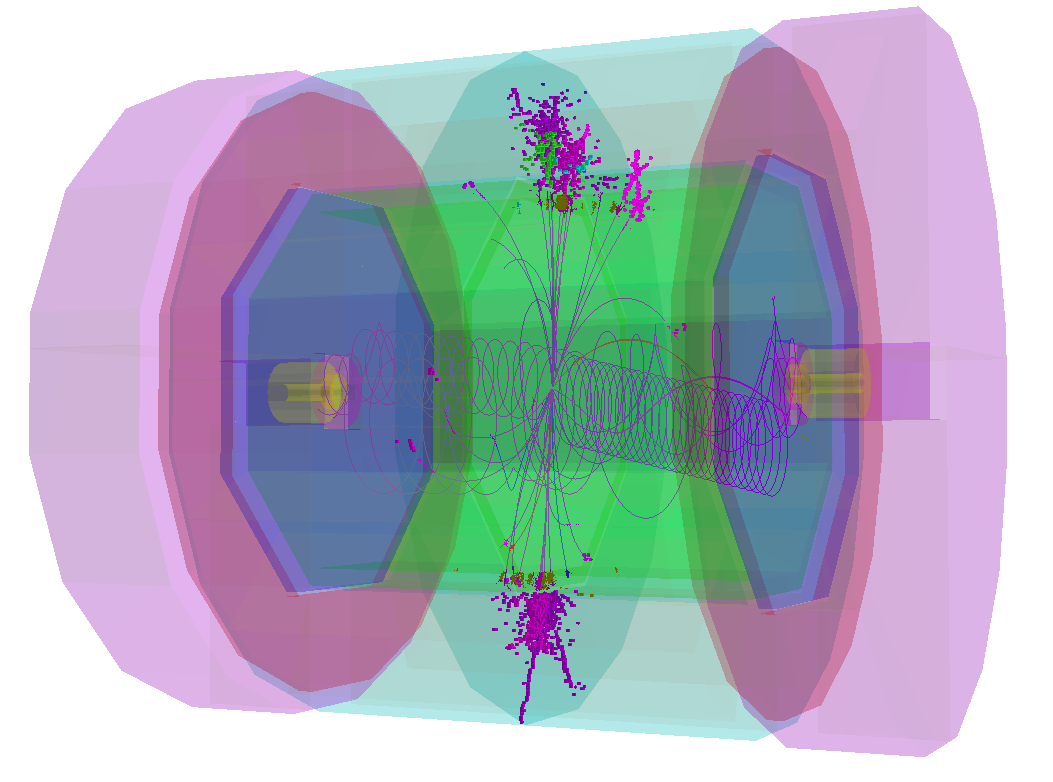
\includegraphics[width=0.5\textwidth]{EnergyEstimators/Plots/SoftComp/VisualDisplay/SoftComp1.png}}
\subfloat[]{\label{fig:softcompclustereventdisplay}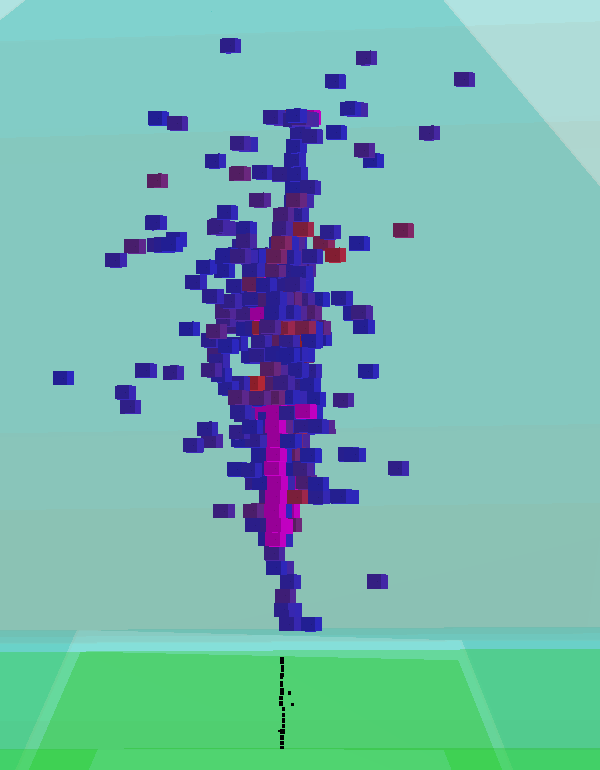
\includegraphics[width=0.3\textwidth]{EnergyEstimators/Plots/SoftComp/VisualDisplay/SoftComp3.png}}
\caption[An event display for a 500 GeV Z$\rightarrow$uds di-jet event reconstructed using the nominal ILD detector.  \protect\subref{fig:softcompfulleventdisplay} shows the full event environment.  \protect\subref{fig:softcompclustereventdisplay} shows a single hadronic cluster from the same event where shading indicates the energy density in the HCal.  High energy density cells are coloured red, while lower energy density cells are coloured blue.  All ECal hits are shaded black.  The high energy density electromagnetic core of the selected hadronic cluster is clearly visible.]{An event display for a 500 GeV Z$\rightarrow$uds di-jet event reconstructed using the nominal ILD detector.  \protect\subref{fig:softcompfulleventdisplay} shows the full event environment.  \protect\subref{fig:softcompclustereventdisplay} shows a single hadronic cluster from the same event where shading indicates the energy density in the HCal.  High energy density cells are coloured red, while lower energy density cells are coloured blue.  All ECal hits are shaded black.  The high energy density electromagnetic core of the selected hadronic cluster is clearly visible.}
\label{fig:softcompeventdisplay}
\end{figure}

This compensation can be applied either at the hardware level, whereby a calorimeter is made to be intrinsically compensating, or at the software level, whereby hadronic showers are identified and their energy estimators modified.  

An example of hardware compensation would be the ZEUS calorimeter \cite{Derrick:1991tq} that was constructed using uranium as the absorber material.  In response to neutral hadrons the uranium underwent fission producing extra energy, which raises the hadronic response of the calorimeter.  The amount of uranium was carefully chosen to achieve a fully compensating calorimeter response i.e. identical calorimeter response to electromagnetic and hadronic showers.  While hardware compensation is possible for the linear collider calorimeters, restrictions on calorimeter construction and the use of a large amount of radioactive material are highly undesirable.  

The high granularity calorimeters and sophisticated pattern recognition software used at the linear collider give excellent resolution on individual particle showers.  This resolution means software compensation can be applied at the linear collider with greater effectiveness than has been possible for previous collider experiments.  

%========================================================================================

\subsection{Application}
The software compensation technique applied in this study involves reweighing HCal hits based on their energy density and the energy of the cluster those hits belong to.  This is applied in the PandoraPFA framework in the form of an energy correction function, which in effect means whenever the energy of a cluster of hits is considered by PandoraPFA the software compensated energy is used.  Applying software compensation in this way benefits the detector energy resolution in two ways; firstly the intrinsic energy resolution of the detector improves and secondly the confusion contribution to the energy resolution, from incorrect association of charged particle tracks to calorimeter hit clusters, is reduced.  Lowering the confusion benefits the energy resolution as it decreases the number calorimeter hits where the energy of the hit is effectively double counted, if charged particle hits are not associated to a track, or not counted at all, if neutral hadron hits are associated to a track.   

Software compensation is applied to clusters of calorimeter hits, as opposed to being applied directly to the final output PFOs, so that the more accurate energy estimators can be used during the reconstruction.  For a cluster of calorimeter hits with an initial energy of $E_{\text{Raw}}$, which is  calculated by summing the calorimeter hit energies, the software compensated cluster energy, $E_{SoftComp}$ \cite{Adloff:2012gv}, is given by 

\begin{equation}
E_{SoftComp} = E_{ECal} + \sum_{i} E_{i} \times \omega_{i}(E_{\text{Raw}}, \rho_{i}) + E_{\text{Muon Chamber}}
\label{equ:softcomp}
\end{equation}

where $E_{ECal}$ is the sum of the calorimeter hit energies measured in the ECal, $E_{i}$ and $\rho_{i}$ are the energy and energy density of HCal hit $i$ respectively, $\omega_{i}$ is the software compensation weight applied to hit $i$, $E_{\text{Muon Chamber}}$ is the cluster energy recorded in the muon chamber and the sum runs over all hits, $i$, in the HCal.  The weight function $\omega_{i}(E_{\text{Raw}}, \rho_{i})$ is defined as

\begin{equation}
\omega_{i}(E_{\text{Raw}}, \rho_{i}) = p_{1}(E_{\text{Raw}}) \times exp(p_{2}(E_{\text{Raw}}) \times \rho_{i}) + p_{3}(E_{\text{Raw}}) \\
p_{1} = p_{11} + p_{12} \times E_{\text{Raw}} + p_{13} \times E_{\text{Raw}}^{2} \\
p_{2} = p_{21} + p_{22} \times E_{\text{Raw}} + p_{23} \times E_{\text{Raw}}^{2} \\
p_{3} = \frac{p_{31}}{p_{32} + exp(p_{33} \times E_{\text{Raw}})}
\label{equ:softcompweight}
\end{equation}

where $p_{ij}$ are trained parameters.  The parameters $p_{ij}$ are determined by performing a $\chi^{2}$ fit of $E_{SoftComp}$ to the MC energy for samples of $K^{0}_{L}$ ranging from 10 to 100 GeV in steps of 10 GeV.  Using the fitted parameters, $p_{1}$,  $p_{2}$ and $p_{3}$ as a function of $E_{\text{Raw}}$ and $\omega(E_{\text{Raw}}, \rho)$ as a function of $\rho$ for various $E_{\text{Raw}}$ are shown in figure \ref{fig:softcompparams} and \ref{fig:softcompweights} respectively.  

\begin{figure}
\subfloat[]{\label{fig:softcompparam1}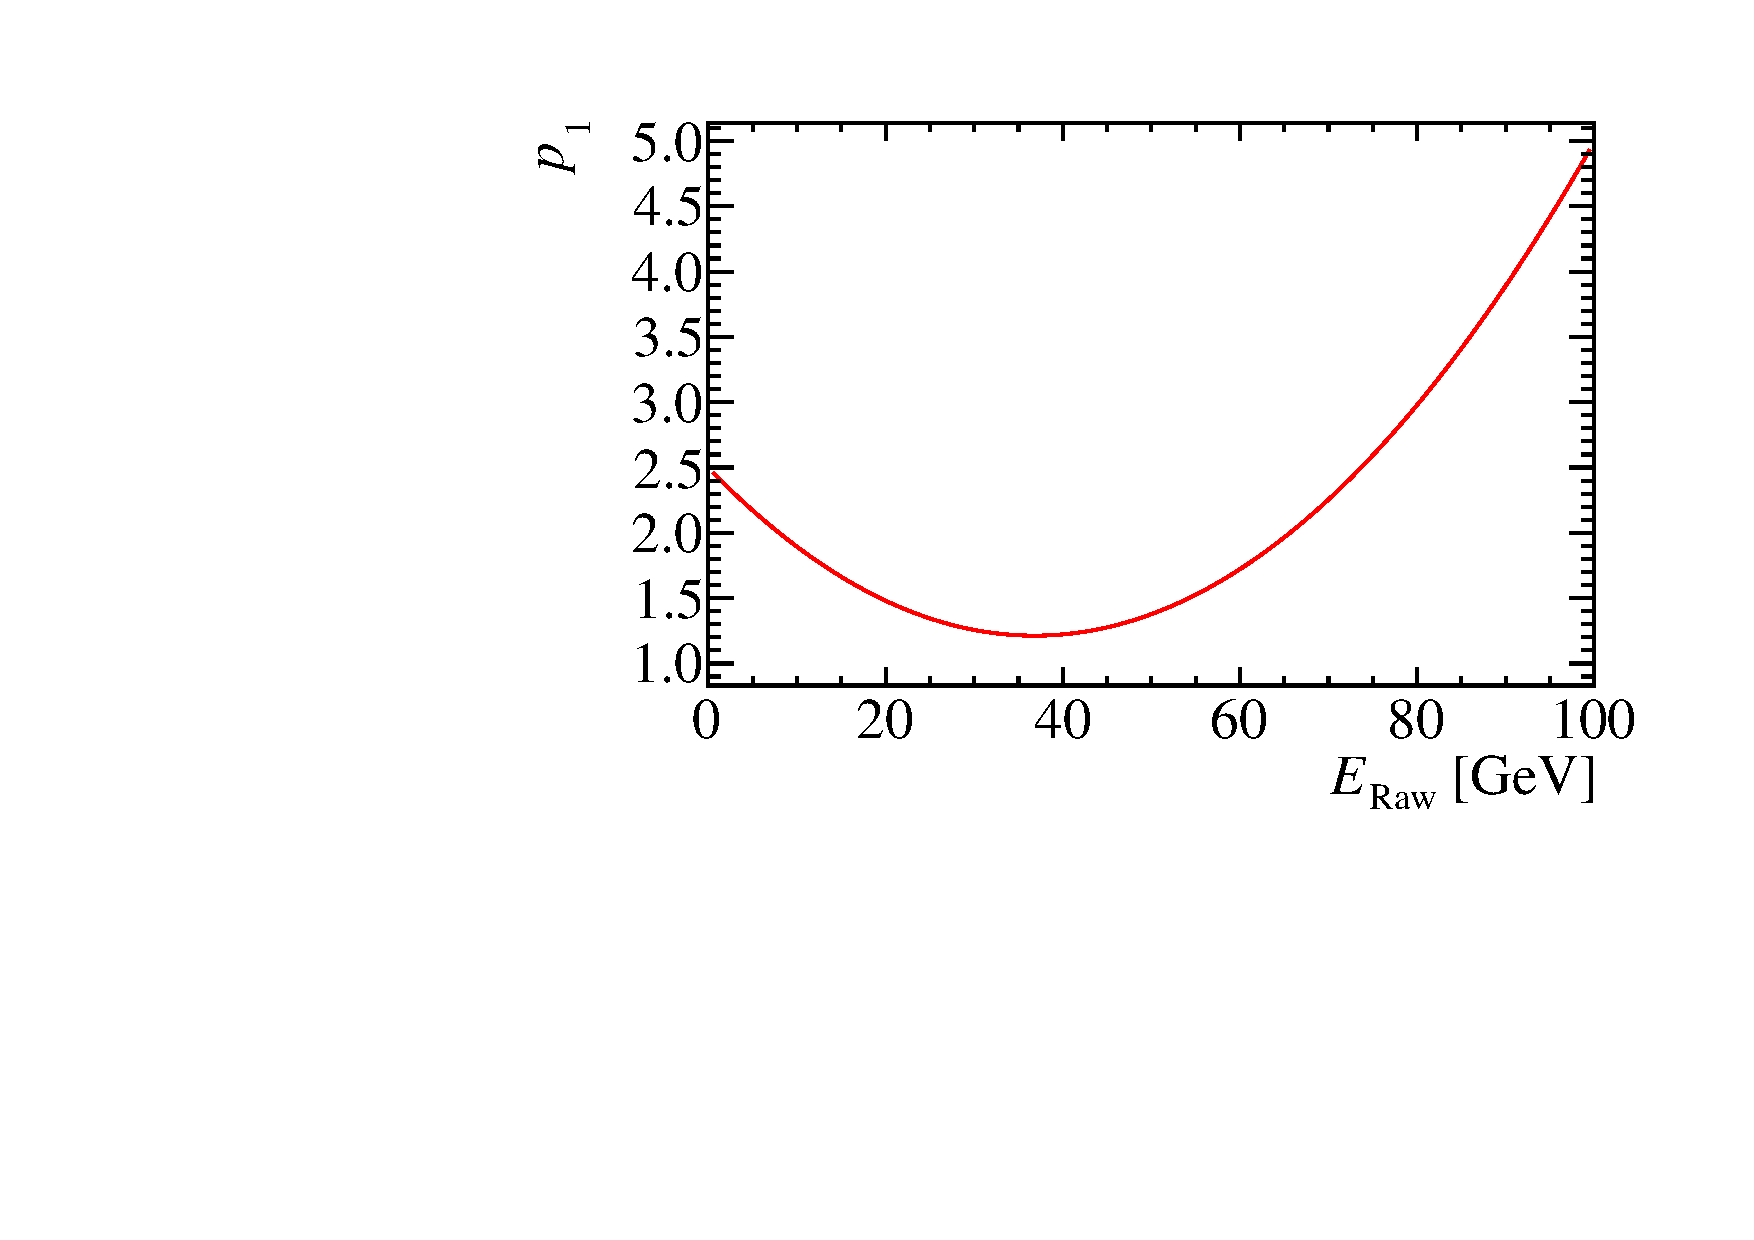
\includegraphics[width=0.33\textwidth]{EnergyEstimators/Plots/SoftComp/Weights/SoftwareCompensationParam1.pdf}}
\subfloat[]{\label{fig:softcompparam2}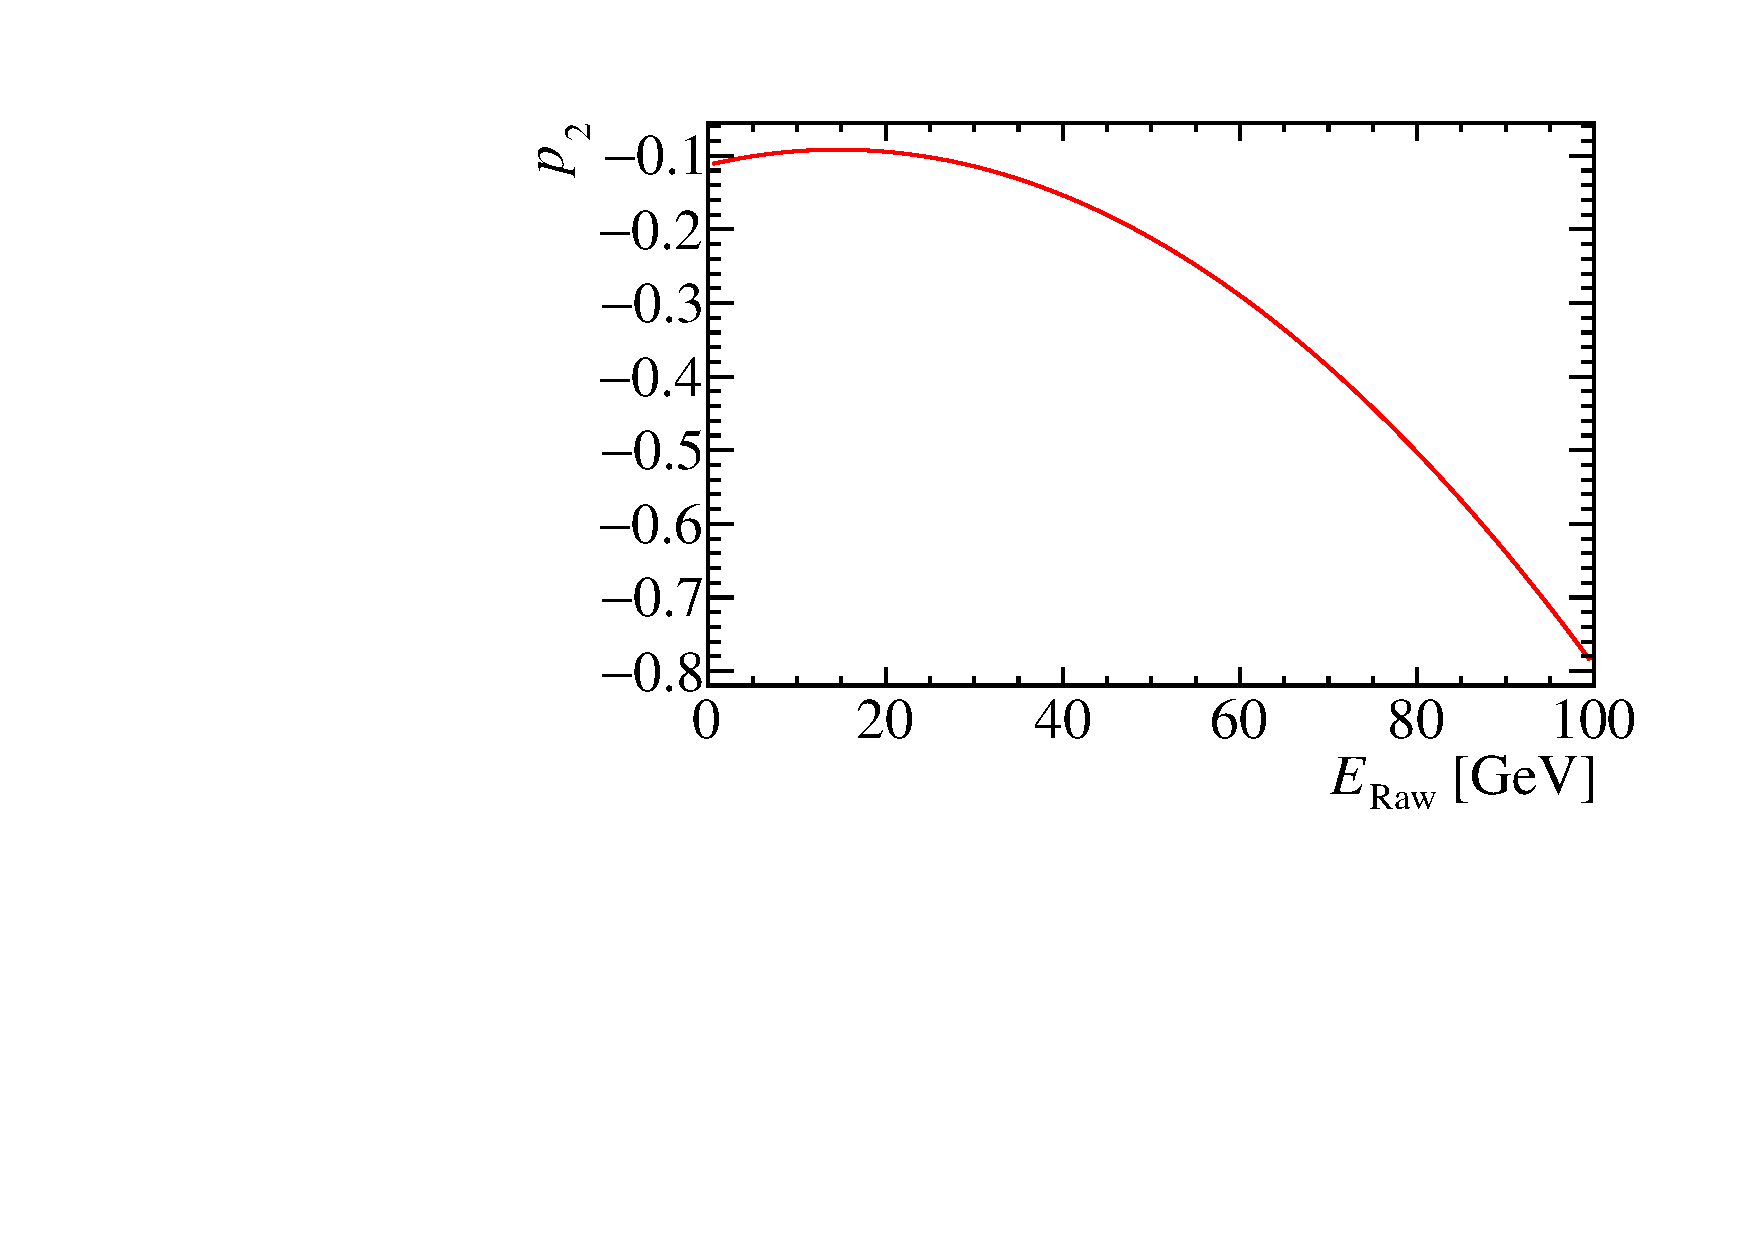
\includegraphics[width=0.33\textwidth]{EnergyEstimators/Plots/SoftComp/Weights/SoftwareCompensationParam2.pdf}}
\subfloat[]{\label{fig:softcompparam3}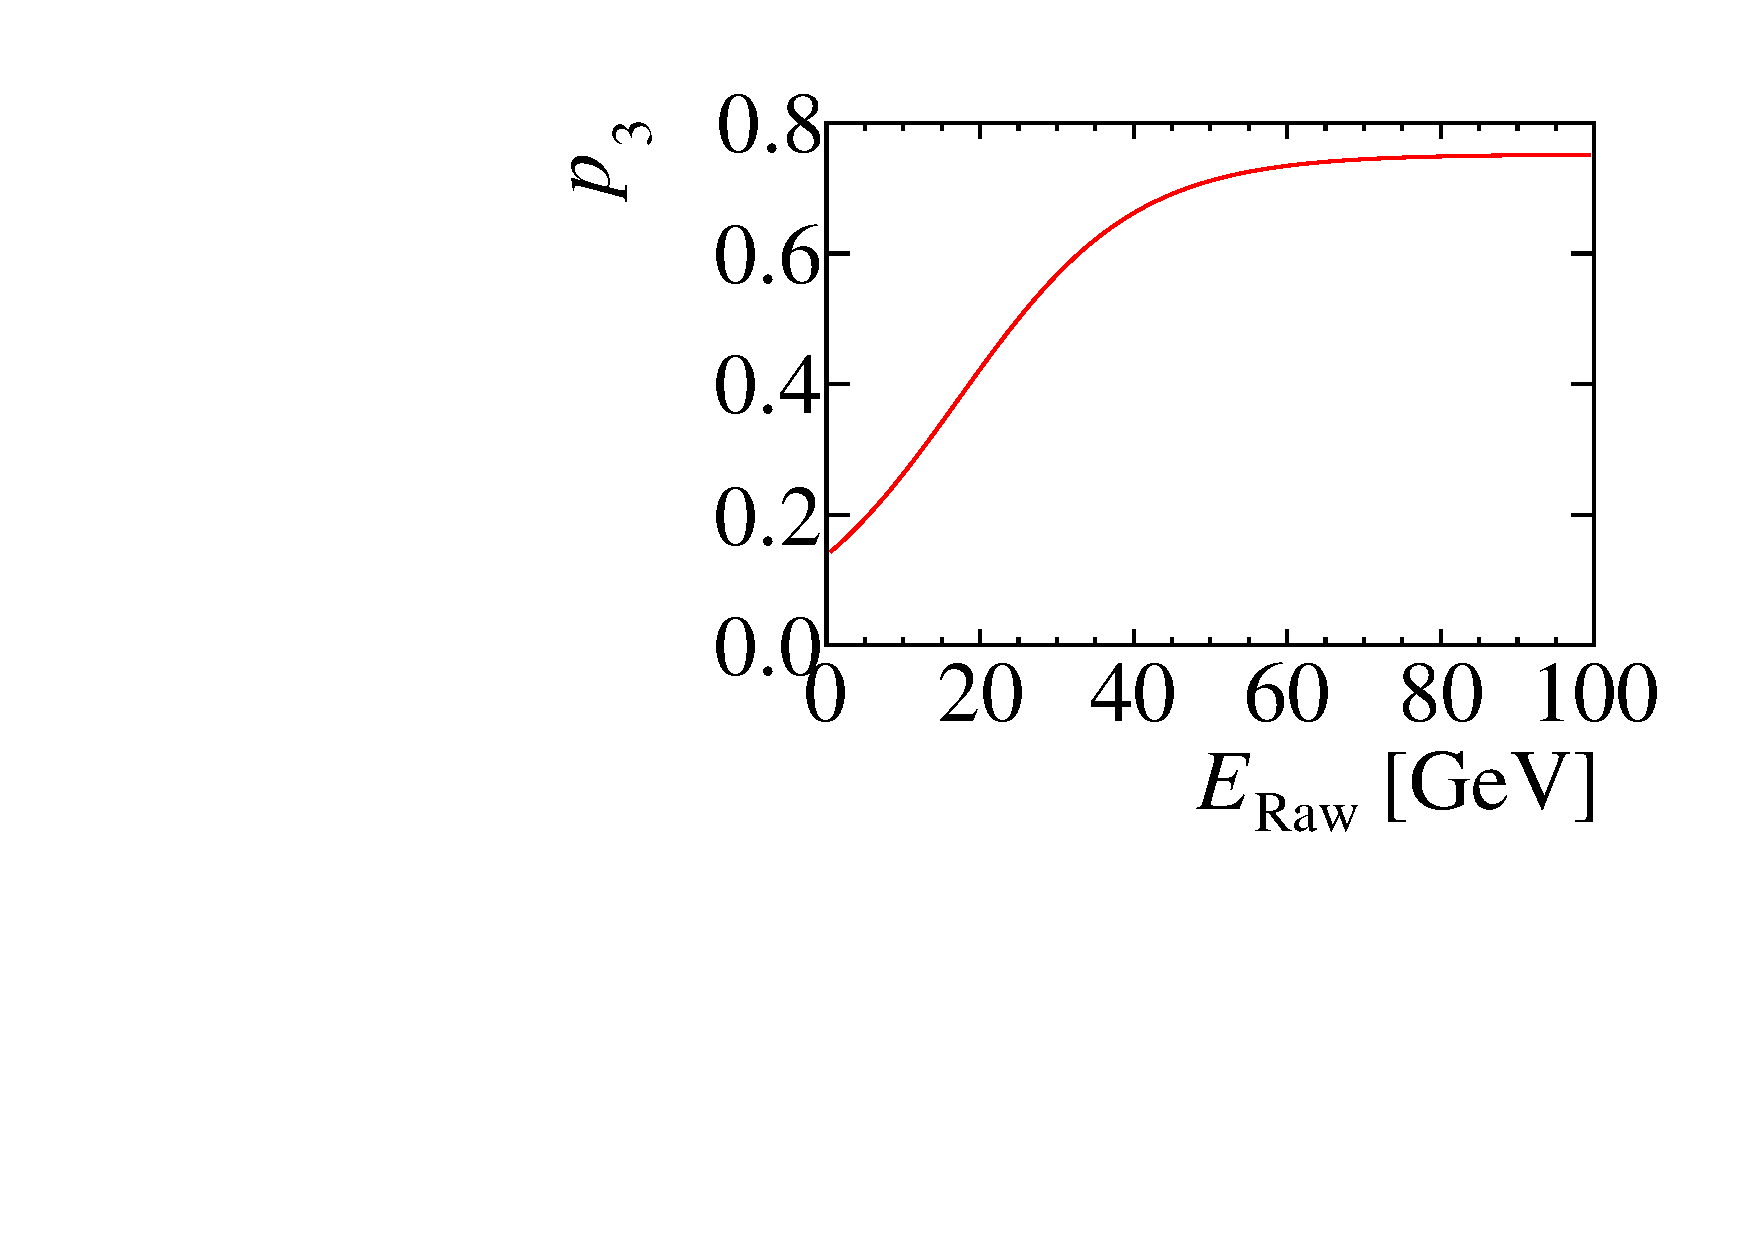
\includegraphics[width=0.33\textwidth]{EnergyEstimators/Plots/SoftComp/Weights/SoftwareCompensationParam3.pdf}}
\caption[]{}
\label{fig:softcompparams}
\end{figure}

\begin{figure}
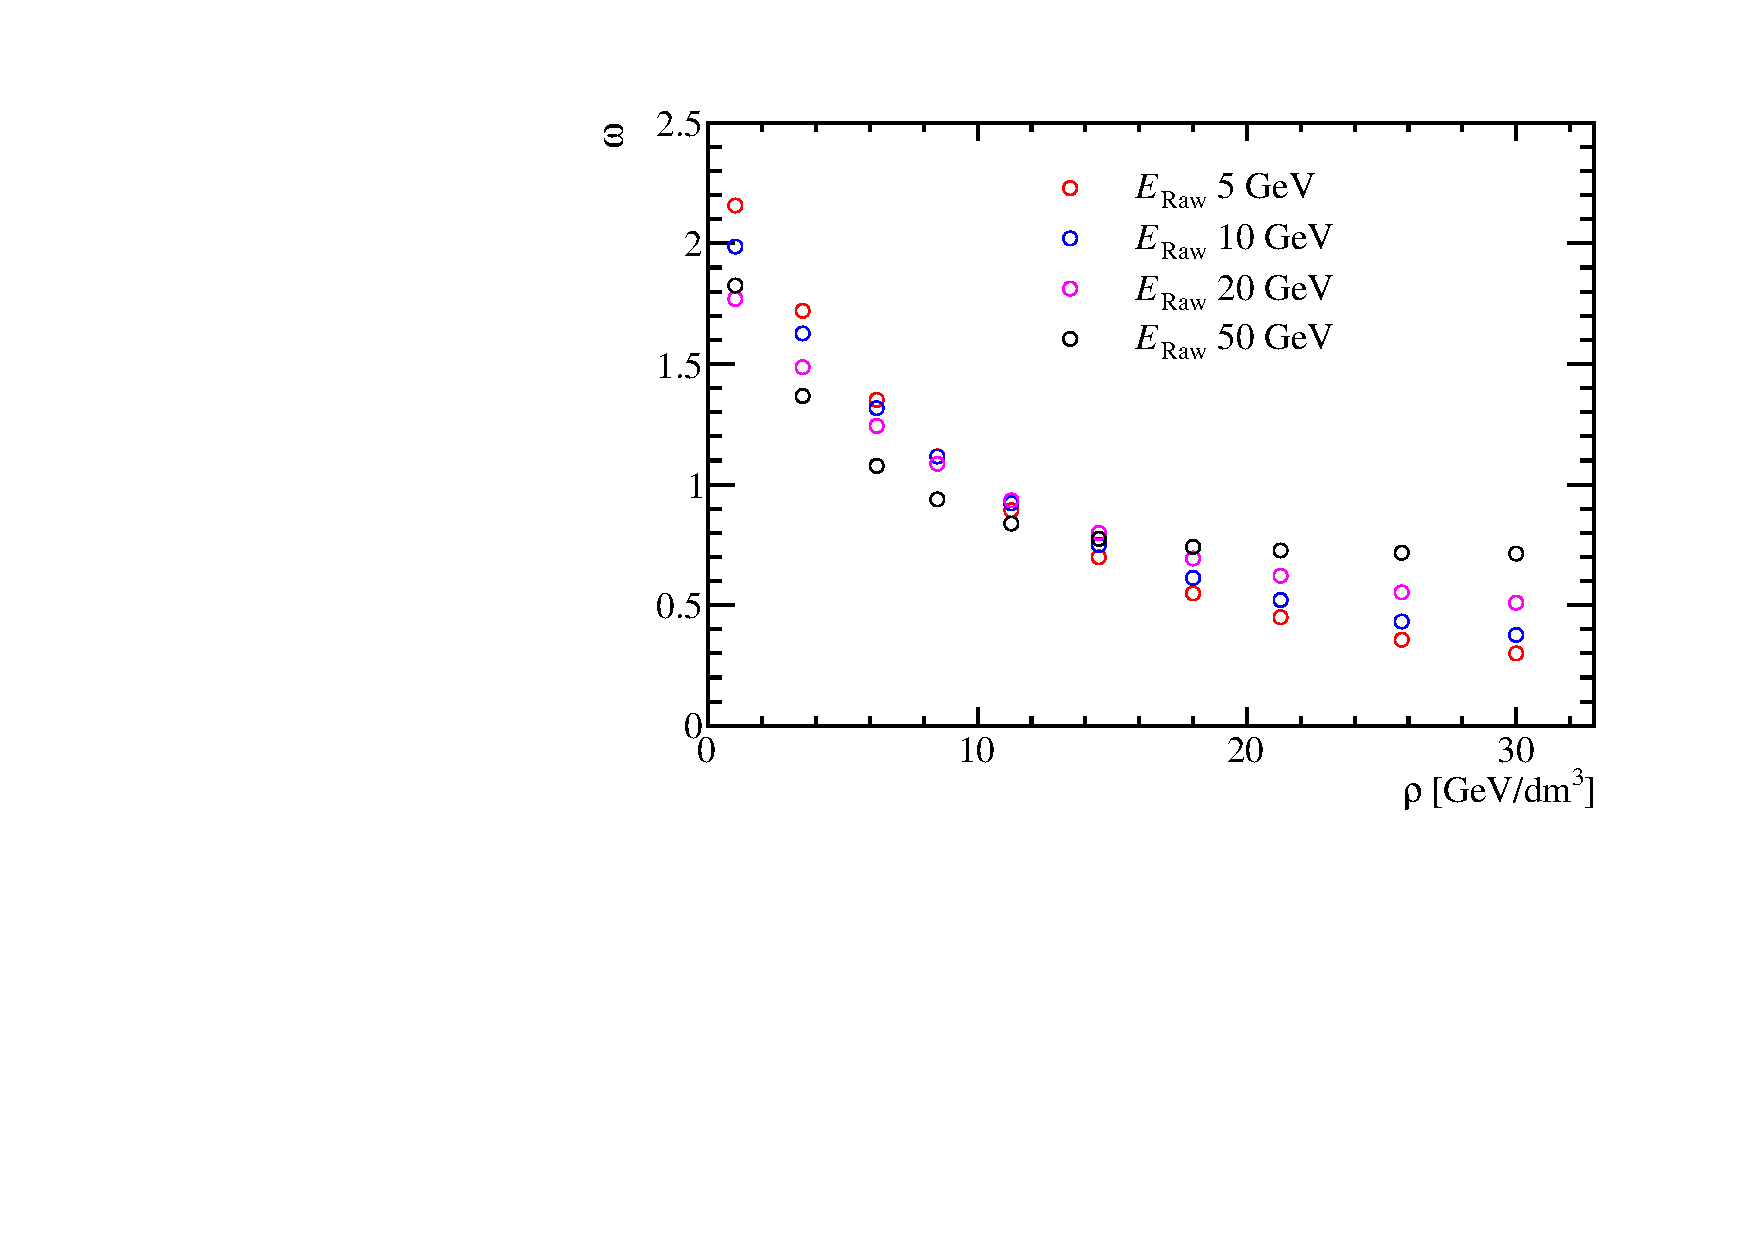
\includegraphics[width=0.5\textwidth]{EnergyEstimators/Plots/SoftComp/Weights/SoftwareCompensationWeights.pdf}
\caption[The software compensation weight applied to a calorimeter hit as a function of calorimeter hit energy density for various cluster energies.]{The software compensation weight applied to a calorimeter hit as a function of calorimeter hit energy density for various cluster energies.}
\label{fig:softcompweights}
\end{figure}

As software compensation only modifies the energy of HCal hits there is freedom to apply further energy corrections to the ECal hits.  Application of the Clean Clusters energy correction logic, described in section \ref{sec:legacycorrections}, to the ECal hits alongside software compensation gave further improvements to the jet energy resolution.  Therefore, as standard the application of software compensation within PandoraPFA implicitly involves the application of the Clean Clusters logic to the ECal hits.  

Software compensation is trained using a maximum $K^{0}_{L}$ energy of 100 GeV, therefor, it is only applied to clusters where $E_{\text{Raw}} < 100$ GeV as the behaviour outside this range cannot be guaranteed.  While it would be possible to modify the energy range of the training sample to go to higher energies, hadronic clusters with energy greater than 100 GeV will be rare for the use case considered here.  This is the case as the ILD detector was designed for use at the ILC, which has a maximum running energy of 500 GeV.  

%========================================================================================

\subsection{Results}

%========================================================================================

\subsubsection{Legacy Energy Corrections}
\label{sec:legacycorrections}
Before examining the impact of software compensation on detector performance is it necessary to address the 'legacy' energy corrections that are used as default in PandoraPFA.  The three energy correction that were in use prior to the development of software compensation are:

\begin{itemize}
\item \textbf{HCal cell truncation}, the details of which can be found in section \ref{sec:hcalcelltruncation}.
\item \textbf{Clean Clusters}.  This algorithm checks to see whether the energy measured within a calorimeter hit is anomalously high.  Anomalously high energy cells are defined as cells where the energy contained within the cell is greater than 10\% of the energy of the cluster that the cell has been associated to.  If a cell is deemed to have an anomalously high energy and if this energy is above a threshold (0.5 GeV) the cell energy used by PandoraPFA is modified.  The updated cell energy is taken as the average cell energy in the calorimeter layers immediately before and after the layer containing the high energy cell.    
\item \textbf{Scale Hot Hadrons}.  This algorithm calculates the average number of MIP equivalent particles passing through each calorimeter cell in a cluster.  If this number is larger than a given value, default 15 MIPs per cell, the cluster energy is rescaled to give a lower average number of MIPs per hit, default is 5 MIPs per hit.  
\end{itemize}

Each of these energy corrections help to deal with the effects of spuriously high energy cells the origin of which is described in section \ref{sec:hcalcelltruncation}.  However, the algorithms are simplistic and software compensation is expected to give far better results than these 'legacy' options.  

The optimisation studies presented in section OPTIMISATION STUDIES use all three of these legacy options simultaneously, which was the default behaviour for PandoraPFA when the studies were undertaken.  The new default behaviour in PandoraPFA is to use software compensation.

%========================================================================================

\subsubsection{Energy Resolution}
\label{sec:softcomper}
The energy resolution as a function of the MC energy for single $K^{0}_{L}$ events is shown in figure \ref{fig:ersoftcomp} using various energy correction settings.  

When comparing the energy resolution given by software compensation to that obtained using no energy corrections, it can be seen that software compensation offers a gain of $\approx 2 \%$ in energy resolution across all energies considered.  The uniformity of this improvement is encouraging, indicating software compensation has been successfully trained across this energy range.   

Comparing the performance of software compensation to the legacy corrections it can be seen that software compensation gives a better energy resolution across almost the entire range of energies considered.  The only exception to this is around $E_{K^{0}_{L}} \approx 50$ where the performance of software compensation and the legacy corrections are comparable.  By removing the cell truncation from the legacy options it is clear that the changes in energy resolution when using the legacy options are being driven by the cell truncation.  This makes the trend in energy resolution observed using the legacy corrections clear as at low $K^{0}_{L}$ energies very few cells are affected by the truncation so the performance is comparable to not using any energy corrections.  At high $K^{0}_{L}$ energies the truncation is too aggressive and removes energy from cells that are not spuriously high leading to a worsening energy resolution.  Between these two extremes, $E_{K^{0}_{L}} \approx 50$, the truncation works ideally and improvement in energy resolution using the legacy corrections is the largest.  

\begin{figure}
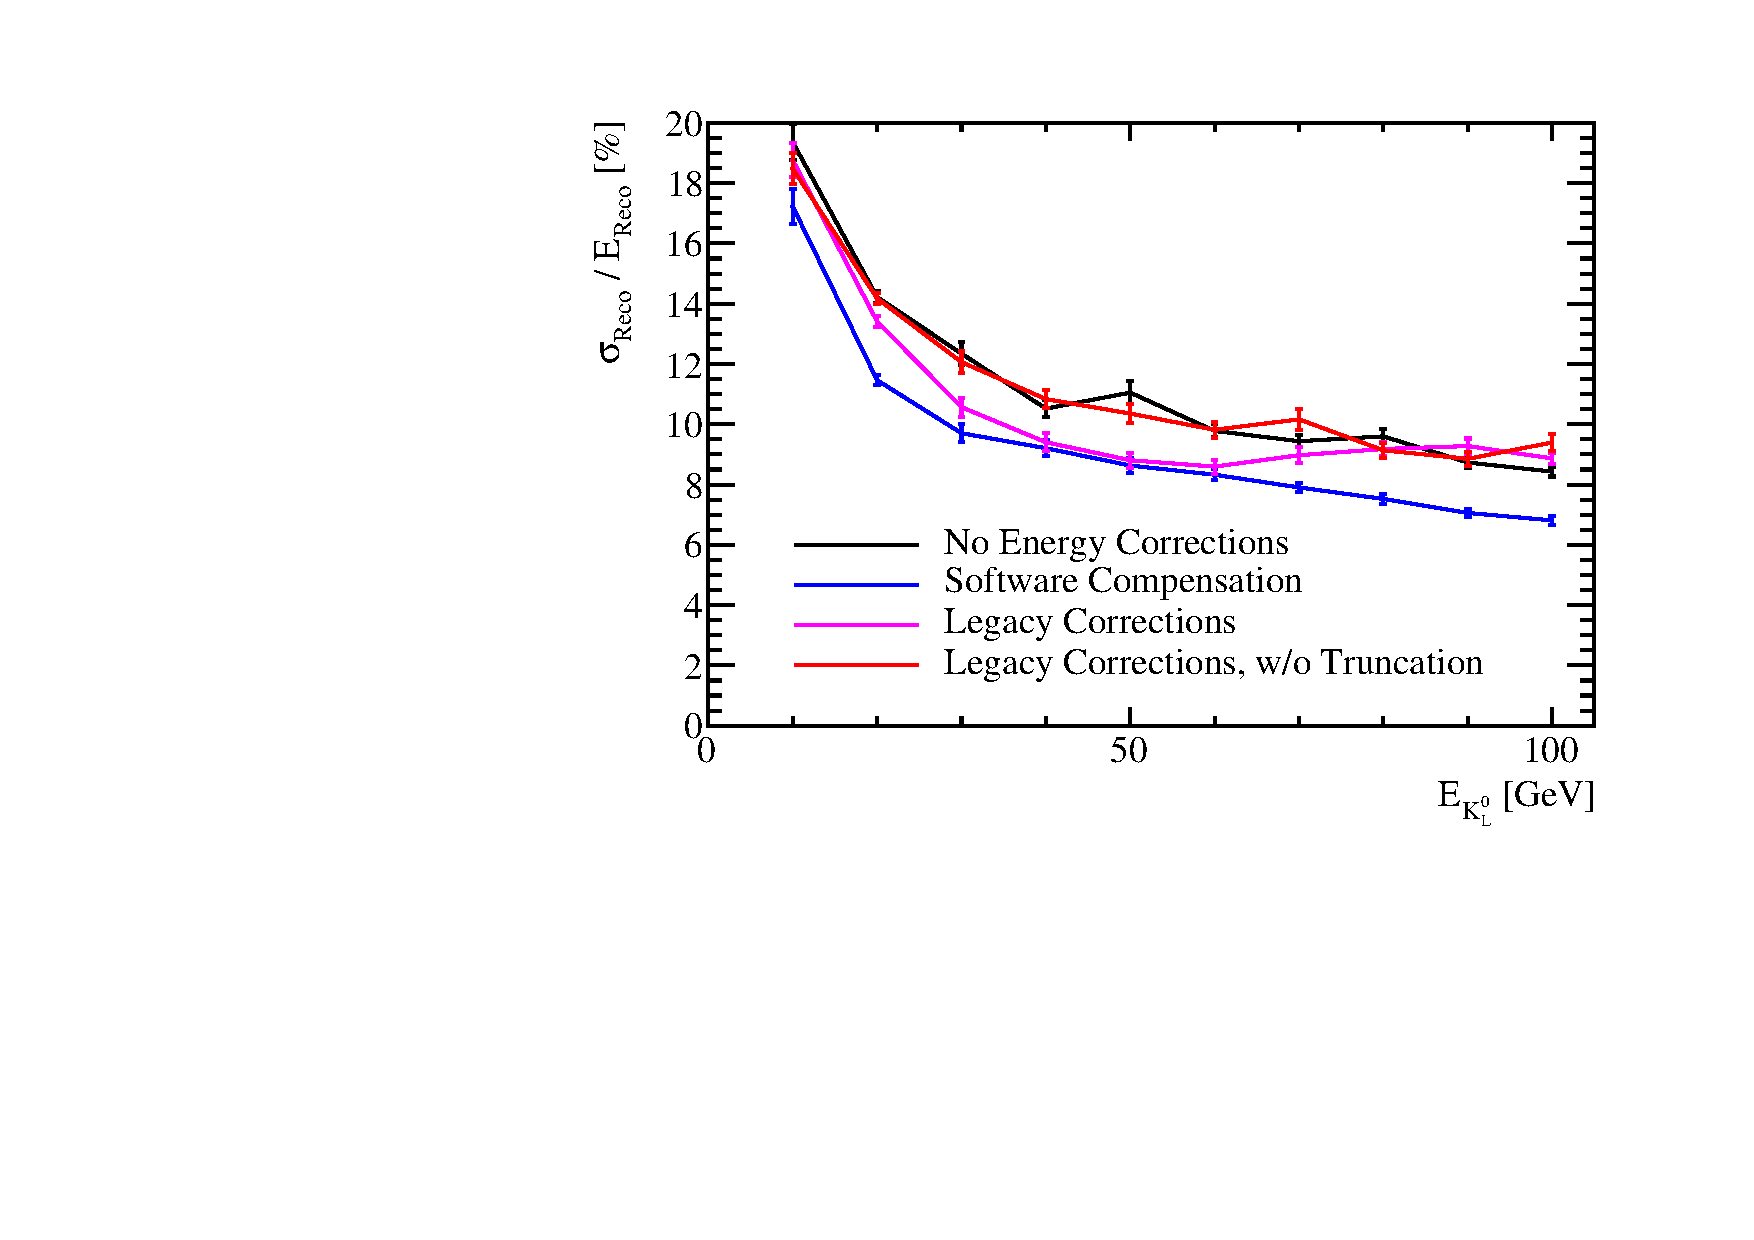
\includegraphics[width=0.5\textwidth]{EnergyEstimators/Plots/SoftComp/EnergyResolution/ER_vs_Kaon0LSoftComp_Kaon0L.pdf}
\caption[The energy resolution as a function of the MC energy for single $K^{0}_{L}$ events using various energy correction settings.  The detector model used was the nominal ILD detector model.]{The energy resolution as a function of the MC energy for single $K^{0}_{L}$ events using various energy correction settings.  The detector model used was the nominal ILD detector model.}
\label{fig:ersoftcomp}
\end{figure}

%========================================================================================

\subsubsection{Jet Energy Resolution}

The improvements in the intrinsic energy resolution of the detector observed when using software compensation will propagate into the reconstruction of jets.  These effects are illustrated by examining the jet energy resolution as a function of jet energy, which is shown in figure \ref{fig:jersoftcomp}.  Again it is clear that software compensation is extremely beneficial to the detector performance.  

\begin{figure}
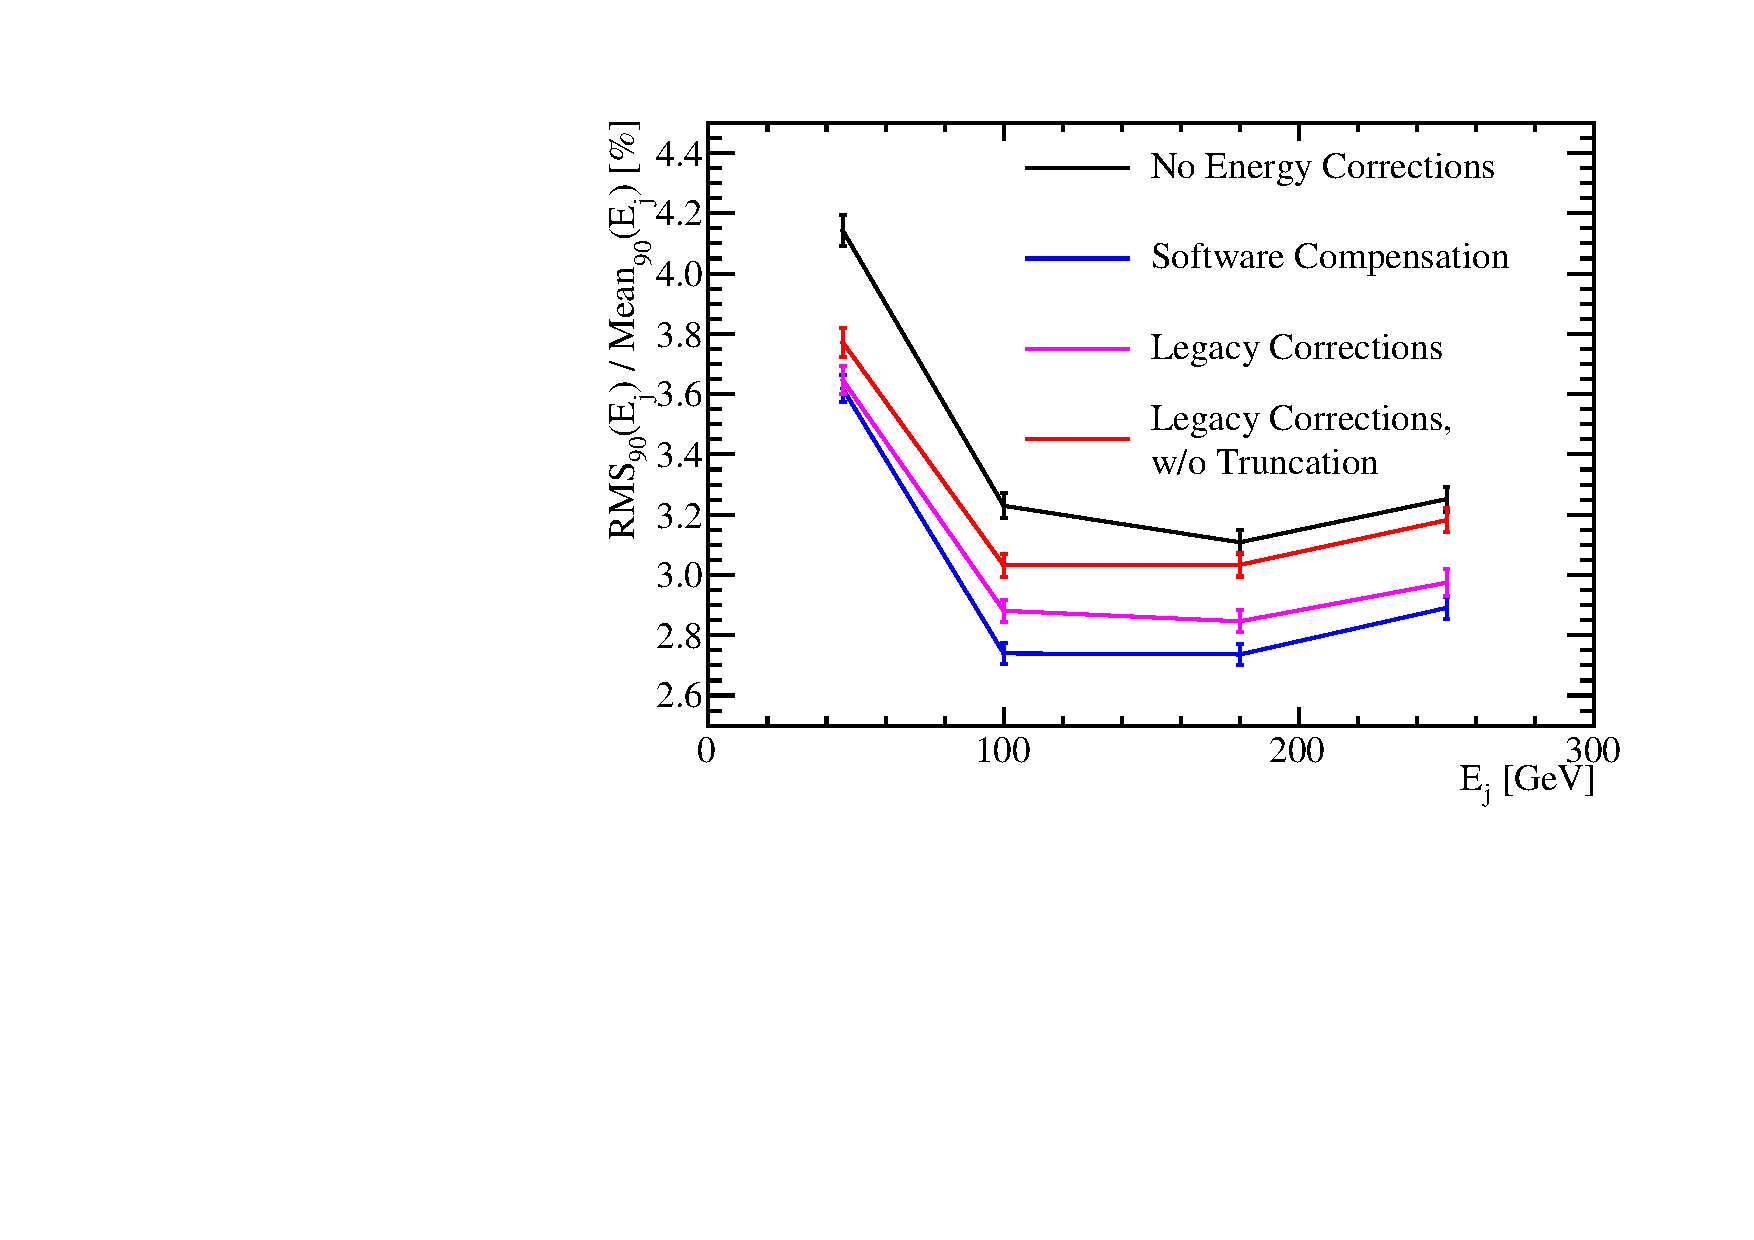
\includegraphics[width=0.5\textwidth]{EnergyEstimators/Plots/SoftComp/JetEnergyResolution/JER_vs_JetEnergy_Default.pdf}
\caption[The jet energy resolution as a function of the jet energy for a variety of different energy correction options.  These results were produced for the nominal ILD detector model.]{The jet energy resolution as a function of the jet energy for a variety of different energy correction options.  These results were produced for the nominal ILD detector model.}
\label{fig:jersoftcomp}
\end{figure}

Software compensation gives a significant reduction in the jet energy resolution in comparison to using no energy corrections.  It also reduces the jet energy resolution in comparison to using the legacy corrections.  

Further light can be shed on these trends by examining the contribution to the jet energy resolutions from the intrinsic energy resolution and the pattern recognition confusion, which are shown in figure \ref{fig:jerbreakdownsoftcomp}.  The intrinsic energy resolution contribution shows that software compensation is significantly better than all other energy corrections options, which is to be expected from the energy resolution studies presented in section \ref{sec:softcomper}.  Unlike the single particle study there is no jet energy for which the cell truncation matches the performance obtained using software compensation.  This is due to the fact that the energy resolution when using the cell truncation is only comparable to the energy resolution using software compensation for a narrow range of hadronic cluster energies.  As the jet contains a broad spectrum of hadronic cluster energies the performance obtained when using the cell truncation will always be worse than when using software compensation.  When comparing the jet energy resolution for the legacy corrections is again apparent that the term driving the jet energy resolution is the cell truncation.

The confusion contribution to the jet energy resolution when using software compensation and the legacy corrections is almost identical.  This indicates that the improvement seen in the jet energy resolution, shown in figure \ref{fig:jersoftcomp}, when using software compensation as opposed to the legacy corrections is being driven by improvements to the intrinsic energy resolution.  

At low jet energies the Clean Clusters and Scale Hot Hadrons energy corrections are beneficial at reducing the confusion contribution, while the cell truncation is largely redundant.  For high jet energies jets this trend is reversed.  As the use of the Clean Clusters and Scale Hot Hadrons energy corrections do not alter the intrinsic energy resolution of the detector it is apparently that these energy corrections are purposed to account for failures in the pattern recognition that occur largely at low jet energies.  On the other hand the cell truncation and software compensation techniques aim to improve the energy resolution of the hadronic clusters, which has a knock-on effect of improving the track cluster associations made in the pattern recognition.  These corrections work across all energy ranges, but have a greater impact at high energies.  

By extracting the Clean Clusters logic, which is the driving term reducing the confusion contribution to the jet energy resolution at low jet energies, and embedding it within the software compensation energy correction, it is possible to achieve exceptional jet energy resolutions that will extend the physics reach of the linear collider detector.  

\begin{figure}
\subfloat[]{\label{fig:jerbreakdownsoftcomp1}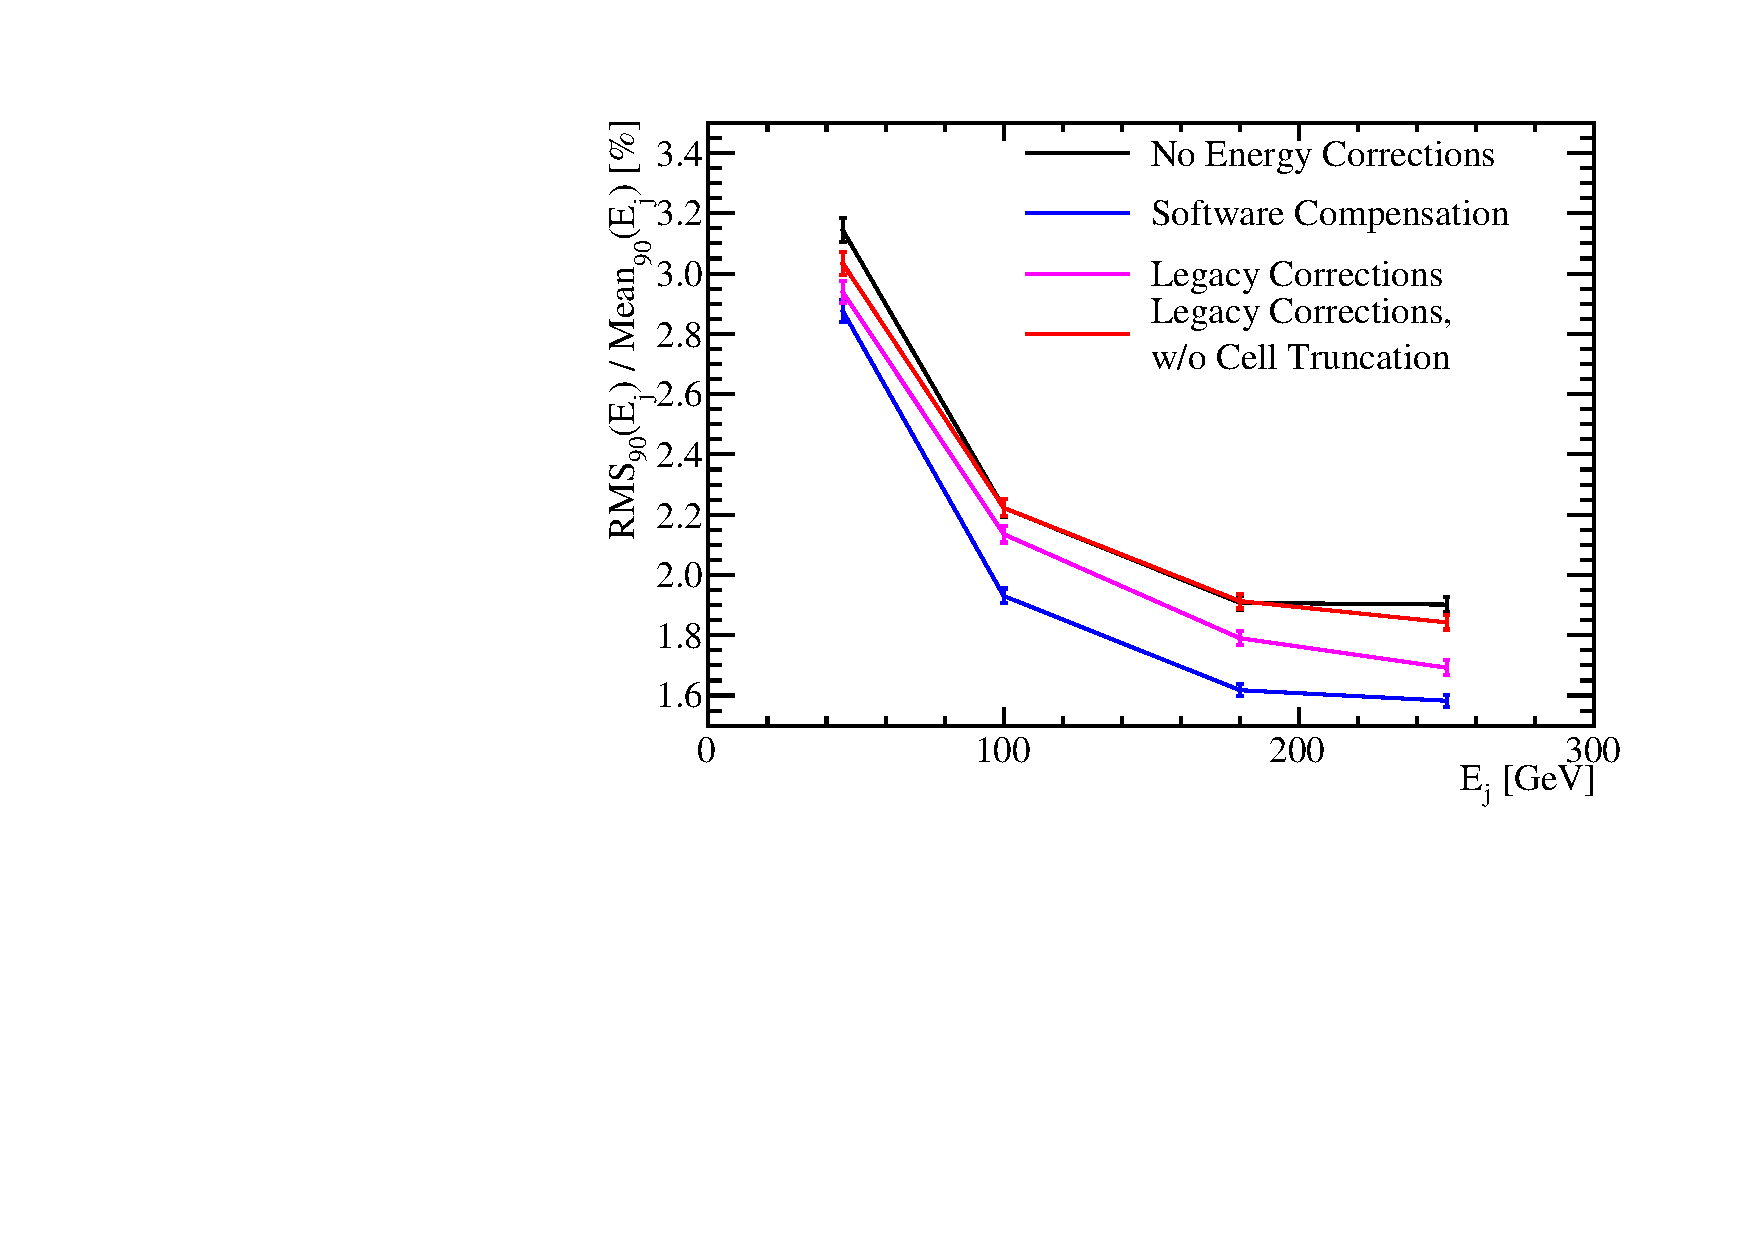
\includegraphics[width=0.5\textwidth]{EnergyEstimators/Plots/SoftComp/JetEnergyResolution/JER_vs_JetEnergy_PerfectPFA.pdf}}
\subfloat[]{\label{fig:jerbreakdownsoftcomp2}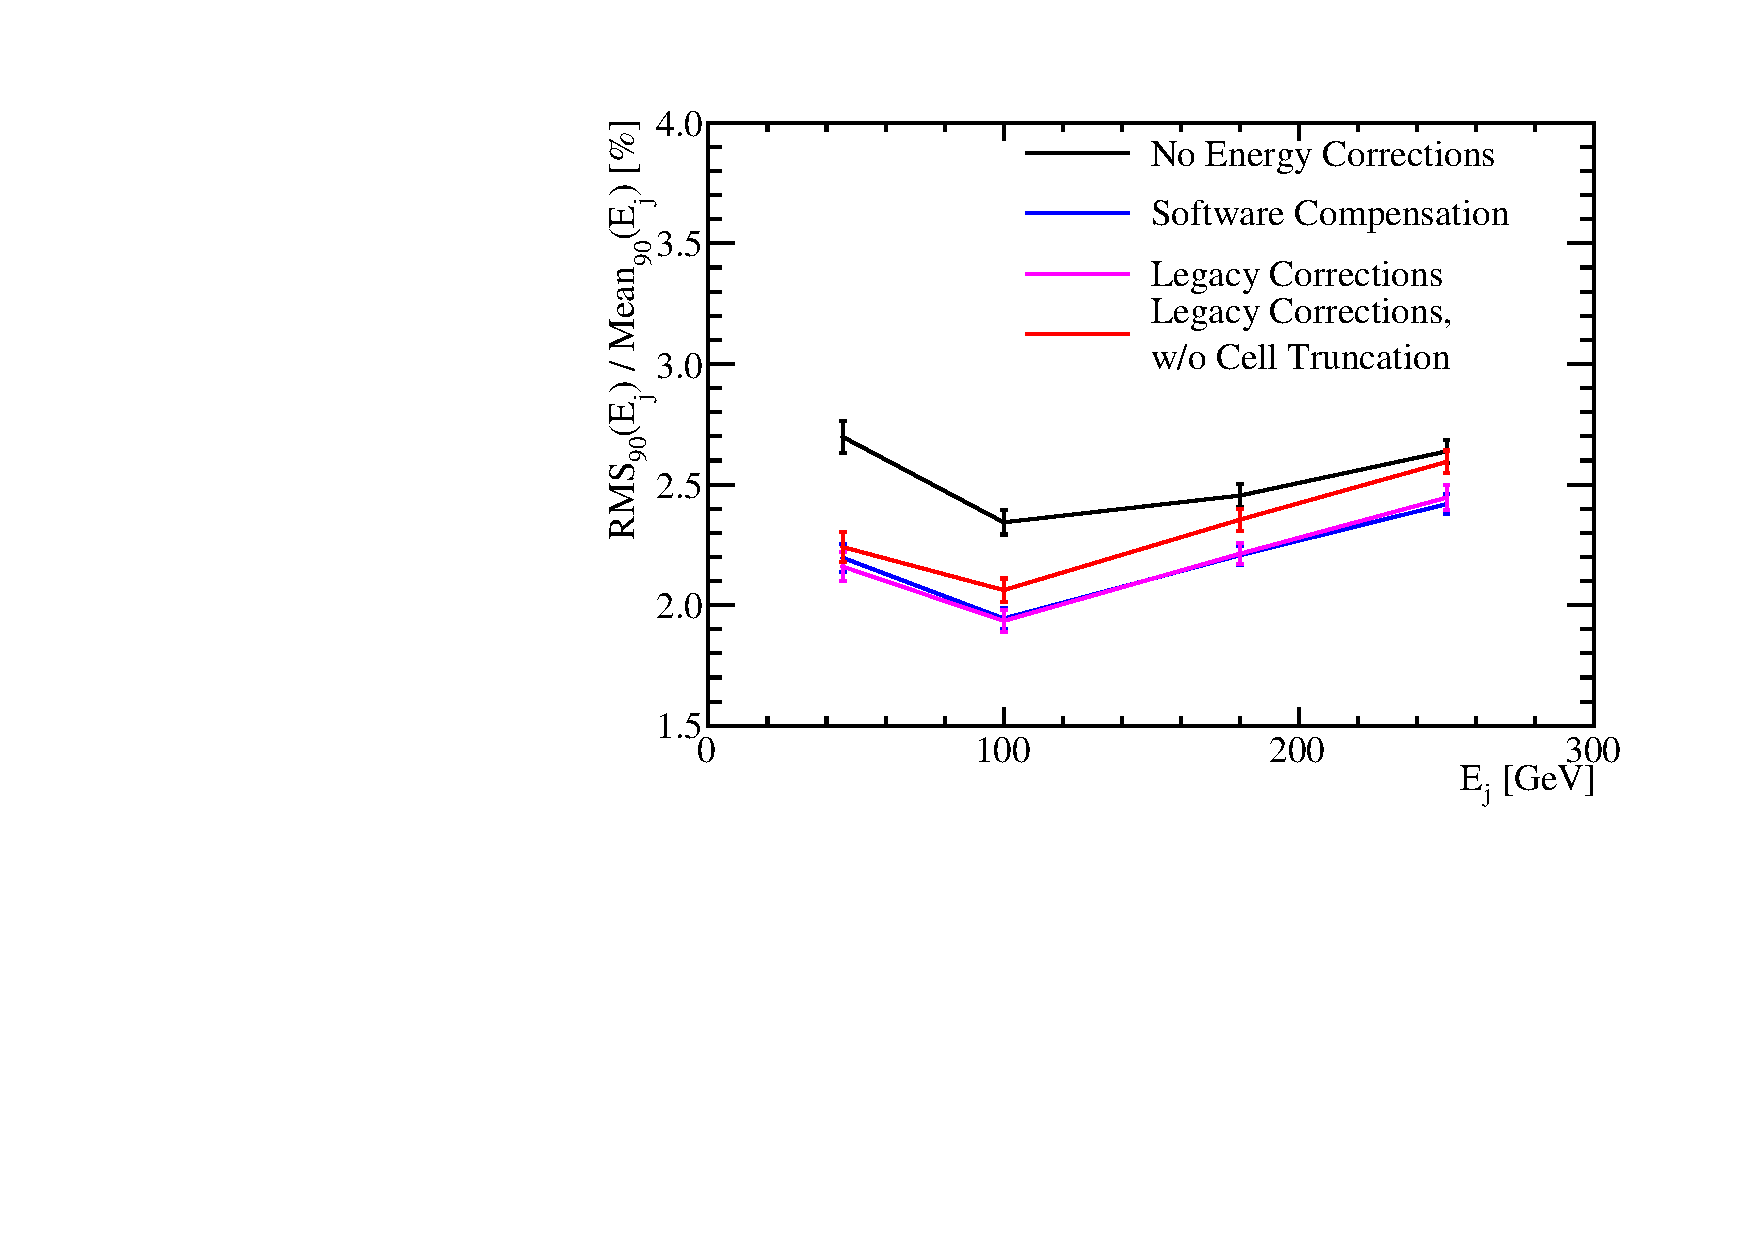
\includegraphics[width=0.5\textwidth]{EnergyEstimators/Plots/SoftComp/JetEnergyResolution/JER_vs_JetEnergy_TotalConfusion.pdf}}
\caption[The contributions to the jet energy resolution as a function of the jet energy for a variety of different energy correction options.  \protect\subref{fig:jerbreakdownsoftcomp1} is the intrinsic energy resolution of the detector and \protect\subref{fig:jerbreakdownsoftcomp2} is the total confusion term.  The quadrature sum of both yields the standard reconstruction performance.  These results were produced for the nominal ILD detector model.]{The contributions to the jet energy resolution as a function of the jet energy for a variety of different energy correction options.  \protect\subref{fig:jerbreakdownsoftcomp1} is the intrinsic energy resolution of the detector and \protect\subref{fig:jerbreakdownsoftcomp2} is the total confusion term.  The quadrature sum of both yields the standard reconstruction performance.  These results were produced for the nominal ILD detector model.}
\label{fig:jerbreakdownsoftcomp}
\end{figure}

%========================================================================================
%========================================================================================

\section{Timing Cuts}
The ILC and CLIC will operate using a trigger-less readout approach whereby the recorded data for each sub-detector is readout between collisions of $\text{e}^{+}$ and $\text{e}^{-}$ bunches.  The train structure for the ILC and CLIC at maximum operating energy is shown in table \ref{table:trainstructure}.  Event selection will proceed through the application of a software trigger.  This involves the identification of hard interactions, prior to full event reconstruction, and only putting data into the event reconstruction if it is measured within a chosen time window about this interaction.  Timing cuts placed on the calorimeter hits are corrected for straight time-of-flight to the IP.  This ensures that the amount of time particle showers have to develop in the calorimeters is independent of their position.  As the size of the time window around the hard interaction changes the amount of time particle showers have to develop varies and this will affect the performance of the detector. 

\begin{table}[h!]
\centering
\begin{tabular}{l r r}
\hline
& ILC 500 GeV & CLIC 3 TeV \\
\hline
Electrons per bunch & 2.0 & 0.37 \\
Bunches per train & 2810 & 312 \\
Train repetition rate [Hz] & 5 & 50 \\
Bunch separation [ns] & 308 & 0.5 \\
\end{tabular}
\caption[The train structure for 500 GeV ILC and 3 TeV CLIC.]{The train structure for 500 GeV ILC and 3 TeV CLIC.  CITE}
\label{table:trainstructure}
\end{table}

For all choices of time window considered in this study the calibration procedure was reapplied.  This means that the mean of the reconstructed energy distributions will be invariant to changes in the calorimeter timing window as the calibration procedure compensates for any energy losses incurred by truncating the particle shower development time.  

The energy resolution for 100 GeV $\gamma$ and 50 GeV $K^{0}_{L}$ events as a function of the timing window applied to the calorimeter hits is shown in figure \ref{fig:ertimingcuts} for the nominal ILD detector model .  The timing cut makes little difference to the energy resolution of the $\gamma$ events as they produce electromagnetic showers that develop rapidly.  However, there is a significant decrease in the energy resolution for the neutral hadrons, which is expected as these showers develop much more slowly.  Truncating the measurement of the hadronic showers by having a small time window leads to a reduced sampling of the shower, as those hits passing the time window are no longer measured, and a broadening of the reconstructed energy distribution.  

\begin{figure}
\subfloat[]{\label{fig:ertimingcutsphotons}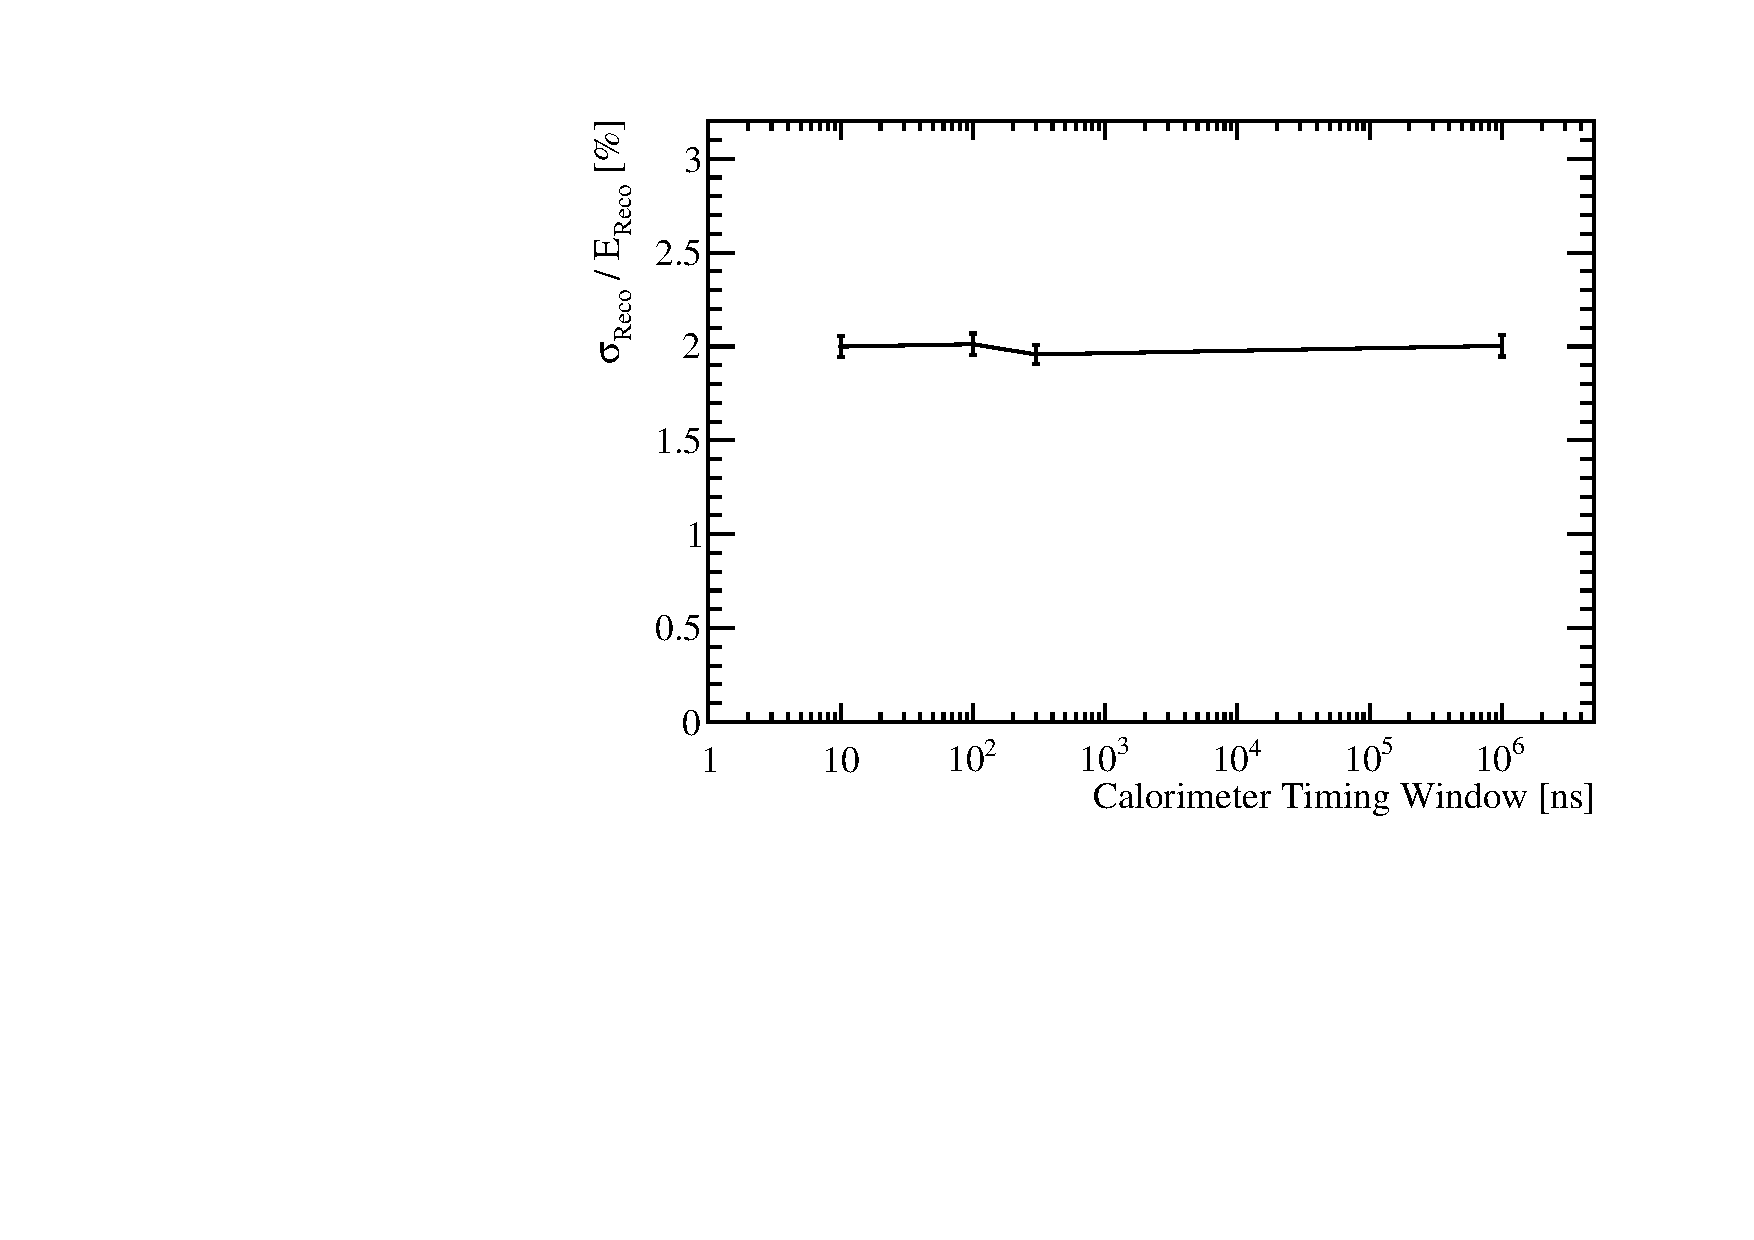
\includegraphics[width=0.5\textwidth]{EnergyEstimators/Plots/TimingCuts/ER_vs_PhotonTiming_100GeVPhoton.pdf}}
\subfloat[]{\label{fig:ertimingcutskaons}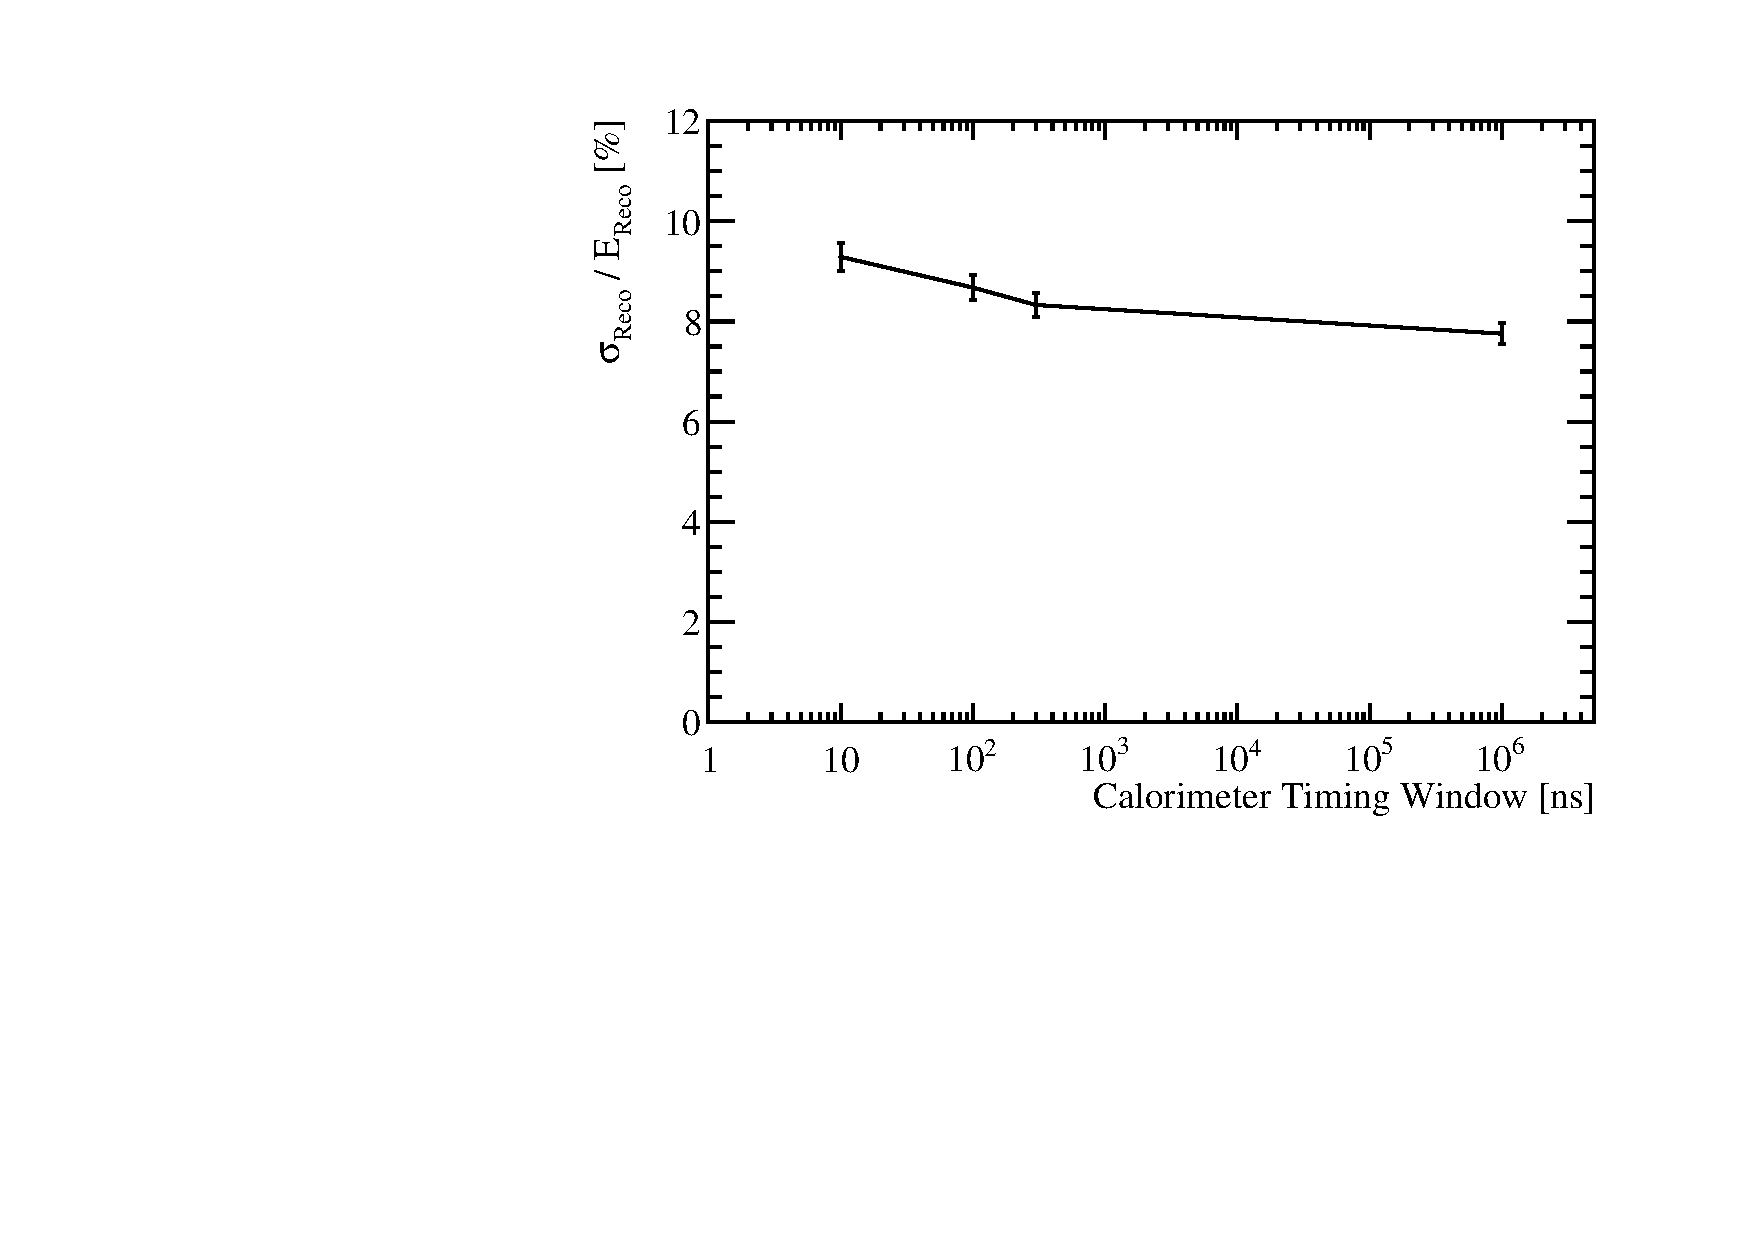
\includegraphics[width=0.5\textwidth]{EnergyEstimators/Plots/TimingCuts/ER_vs_Kaon0LTiming_50GeVKaon0L.pdf}}
\caption[The energy resolution as a function of calorimeter timing window for \protect\subref{fig:ertimingcutsphotons} 100 GeV $\gamma$ events and \protect\subref{fig:ertimingcutskaons} 50 GeV $K^{0}_{L}$ events for the nominal ILD detector model.]{The energy resolution as a function of calorimeter timing window for \protect\subref{fig:ertimingcutsphotons} 100 GeV $\gamma$ events and \protect\subref{fig:ertimingcutskaons} 50 GeV $K^{0}_{L}$ events for the nominal ILD detector model.}
\label{fig:ertimingcuts}
\end{figure}

The degradation in neutral hadron energy resolution with decreasing calorimeter time window also affects the jet energy resolution, which can be seen in figure \ref{fig:jertimingcuts}.  The sole exception to this is the 250 GeV jets for the 100 ns time window whereby the jet energy resolution is slightly better than when using the 300 ns and semi-infinite time windows.  As the magnitude of the changes to the jet energy resolution when varying the time window size are small in comparison to the absolute resolutions, this exception will most likely be due to a fluctuation in either the event sample used or in the reapplication of the calibration procedure.  

\begin{figure}
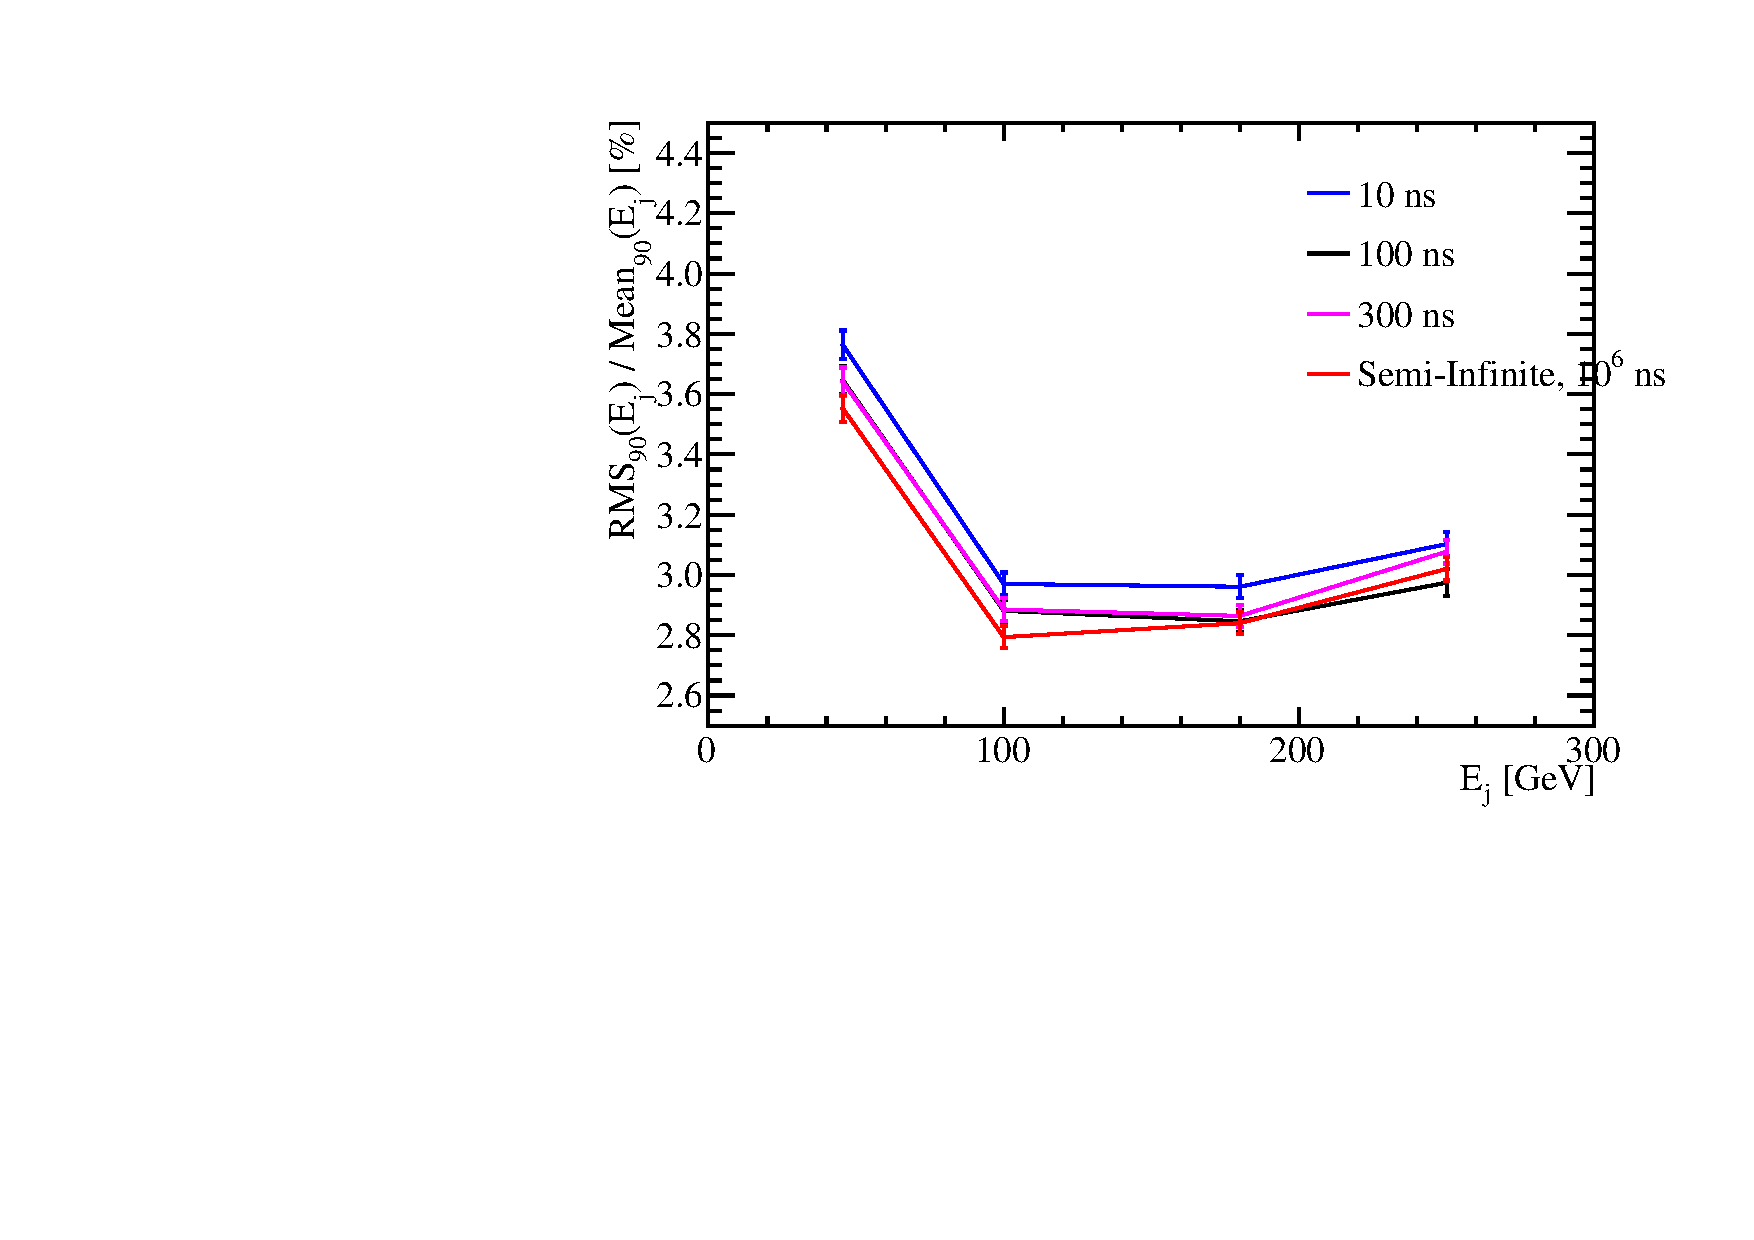
\includegraphics[width=0.5\textwidth]{EnergyEstimators/Plots/TimingCuts/JER_vs_JetEnergy_TimingCutStudies.pdf}
\caption[The jet energy resolution as a function of jet energy for various calorimeter timing cuts.  The results shown use the nominal ILD detector model.]{The jet energy resolution as a function of jet energy for various calorimeter timing cuts.  The nominal ILD detector model was used for this study.}
\label{fig:jertimingcuts}
\end{figure}

The time window applied to the calorimeter hits affects both the neutral hadron and jet energy resolutions with a larger timing window leading to better resolutions.  It can be seen that applying an aggressive choice of time window, such as 10 ns, damages the jet energy resolutions as many of the hadronic showers being sampled do not have time to fully develop.  However, even using a 10 ns timing cut the jet energy resolutions are still sufficiently low to give excellent detector performance.  Both the single particle and jet energy resolutions indicate that the majority of hadronic showers will have fully developed within 100 ns and that there are little gains to be made by extending the size of this window.  

For results presented in this chapter and the optimisation studies found in chapter OPT STUDIES a 100 ns timing window was applied across all models considered.  As the choice of timing window has yet to be finalised for the linear collider this value was chosen as it represents something that could be achieved using the readout technology options presently available CITE.  Furthermore, it adds additional realism to the detector simulation in comparison to omitting the effect of the calorimeter time window.  The categorisation of changes to the detector performance when varying the calorimeter timing window presented here can be used to discern the impact of changing the timing window used for the optimisation studies at a later date if so desired.  

%========================================================================================
%========================================================================================
